\documentclass[hyperref=colorlinks]{beamer}
\mode<presentation>
\usetheme{iclpt}
\setbeamertemplate{navigation symbols}{}
\setbeamertemplate{headline}{
\begin{beamercolorbox}[leftskip=.2cm,rightskip=.2cm,topskip=.2cm,ht=1.1cm,dp=0.1cm,wd=\textwidth]{institute in head/foot}
  
\includegraphics[height=1cm]{icl.pdf}
  \hfill
  
\includegraphics[height=1cm]{../Pics/CMS-Color.pdf}
\end{beamercolorbox}
}
\setbeamertemplate{footline}{
\begin{beamercolorbox}[ht=.55cm,dp=0.4cm,wd=\textwidth,leftskip=.3cm]{author in head/foot}%
  \begin{minipage}[c]{5cm}%
    \usebeamerfont{author in head/foot}
    \insertshortauthor 
    \insertshorttitle
    \end{minipage}\hfill%
  \insertframenumber{} / \pageref{lastframe}
  \hfill
  \begin{minipage}{6cm}
    \hfill
  \end{minipage}
\end{beamercolorbox}%
}

\usepackage{color}
\usepackage{tabularx,colortbl}
\usepackage{graphicx}
\usepackage{pdfpages}
\usepackage{feynmp}
\DeclareGraphicsRule{*}{mps}{*}{}

\title{\vspace{-0.2cm} Control Plots and Trigger Efficiencies}
%\subtitle{Paper - HIG-13-030, PASs: HIG-13-013, HIG-13-018, HIG-13-028 \vspace{-0.7cm}}
\author[P. Dunne]{\underline{P. Dunne} }%\\ on behalf of the H$\rightarrow$invisible analysis groups} % A.M. Magnan and A. Nikitenko Joao Pela with \\ R. Aggleton, J. Brooke: Bristol \\ C.Asawangtrakuldee, Q.Li: Peking \\ P. Srimanobhas: Chulalongkorn \\ S. Kumar, K. Mazumdar: Mumbai}
\titlegraphic{
  \vspace{-0.7cm}
  %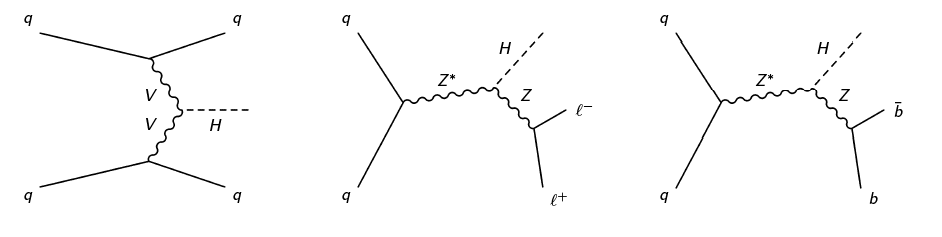
\includegraphics[width=\textwidth]{TalkPics/invcomb021213/feyndiags}
%% \begin{fmfgraph*}(100,70)
%%         \fmfleft{i1,i2}
%%         \fmfright{o1,o2,o3}
%%         \fmf{fermion}{i1,v1,o1}
%%         \fmf{fermion}{i2,v2,o3}
%%         \fmf{phantom,tension=4/5}{v1,v2}
%%         \fmffreeze
%%         \fmf{photon,label=$W,,Z$}{v1,v3}
%%         \fmf{photon,label=$W,,Z$}{v2,v3}
%%         \fmf{dashes}{v3,o2}
%%         \fmflabel{$q$}{i1}
%%         \fmflabel{$q$}{i2}
%%         \fmflabel{$q$}{o1}
%%         \fmflabel{$q$}{o3}
%%         \fmflabel{$H$}{o2}
%%       \end{fmfgraph*}
}
\date{}
\begin{document}
\begin{fmffile}{hig1330approvalfeynmandiags}

%TITLE PAGE
\section{Title}
\begin{frame}
  \titlepage
  
\end{frame}

%OUTLINE
\begin{frame}
  \frametitle{Overview}
  \begin{block}{}
    \scriptsize
    \begin{itemize}
      \item Changes since last time:
      \item[-] Minor bug in lepton weights fixed
      \item[-] Not showing/looking at signal region plots
      \item New ``2D binned'' trigger weights studied
      \item Looked into explanations for munu shape disagreement
    \end{itemize}
  \end{block}
\end{frame}

\begin{frame}
  \frametitle{New Control Plots}
    \begin{block}{}
      \scriptsize
      \begin{itemize}
      \item Cuts applied in all following plots are:
      \item[-] metnomu$>90$ $jet_{1} p_{t}>50$, $\Delta\eta_{jj}>3.6$, metnomu\_significance$>3$, $jet_{1,2} \eta <4.7$, $jet_{1}\eta\cdot jet_{2}\eta<0,m_{jj}>=800,jet_{2} p_{T}>40$, $min(\Delta\phi(alljets\,p_{T}>30,metnomu))>1.0$
      \item[-] taunu region has additional $m_{T}>20$
      \end{itemize}
    \end{block}
\end{frame}


%!!FINE TO HERE
%!!DISCUSSION OF NEW TRIG EFF METHOD
\begin{frame}
  \frametitle{New Trigger Efficiency Method}
  \begin{block}{}
    \scriptsize
    \begin{itemize} 
    \item Previously used 1D efficiencies
    \item[-] weight was product of fitted 1D weights for Jet 2 pt, met and mjj
    \item This ignores any correlations between variables
    \item New method is to measure met efficiency in bins of Jet 2 pt and mjj
    \item[-] Takes correlations into account
    \item[-] Binning increases statistical uncertainties
    \end{itemize}
  \end{block}
  \begin{block}{}
    \begin{tabular}{|l|c|c|c|c|c|}
      \hline
      j2pt$\backslash$mjj & 0-600 & 600-800 & 800-900 & 900-1000 & 1000-5000 \\
      \hline
      30-40 &11&12&13&14&15\\
      \hline
      40-50 &21&22&23&24&25\\
      \hline
      50-60 &31&32&33&34&35\\
      \hline
      60-500 &41&42&43&44&45\\
      \hline
    \end{tabular}
  \end{block}
\end{frame}


%!!SHOW A FEW TRIGGER EFF CURVES
\begin{frame}
  \frametitle{Trigger Efficiency Curves}
  \begin{columns}
    \column{.5\textwidth}
    \begin{block}{Good}
      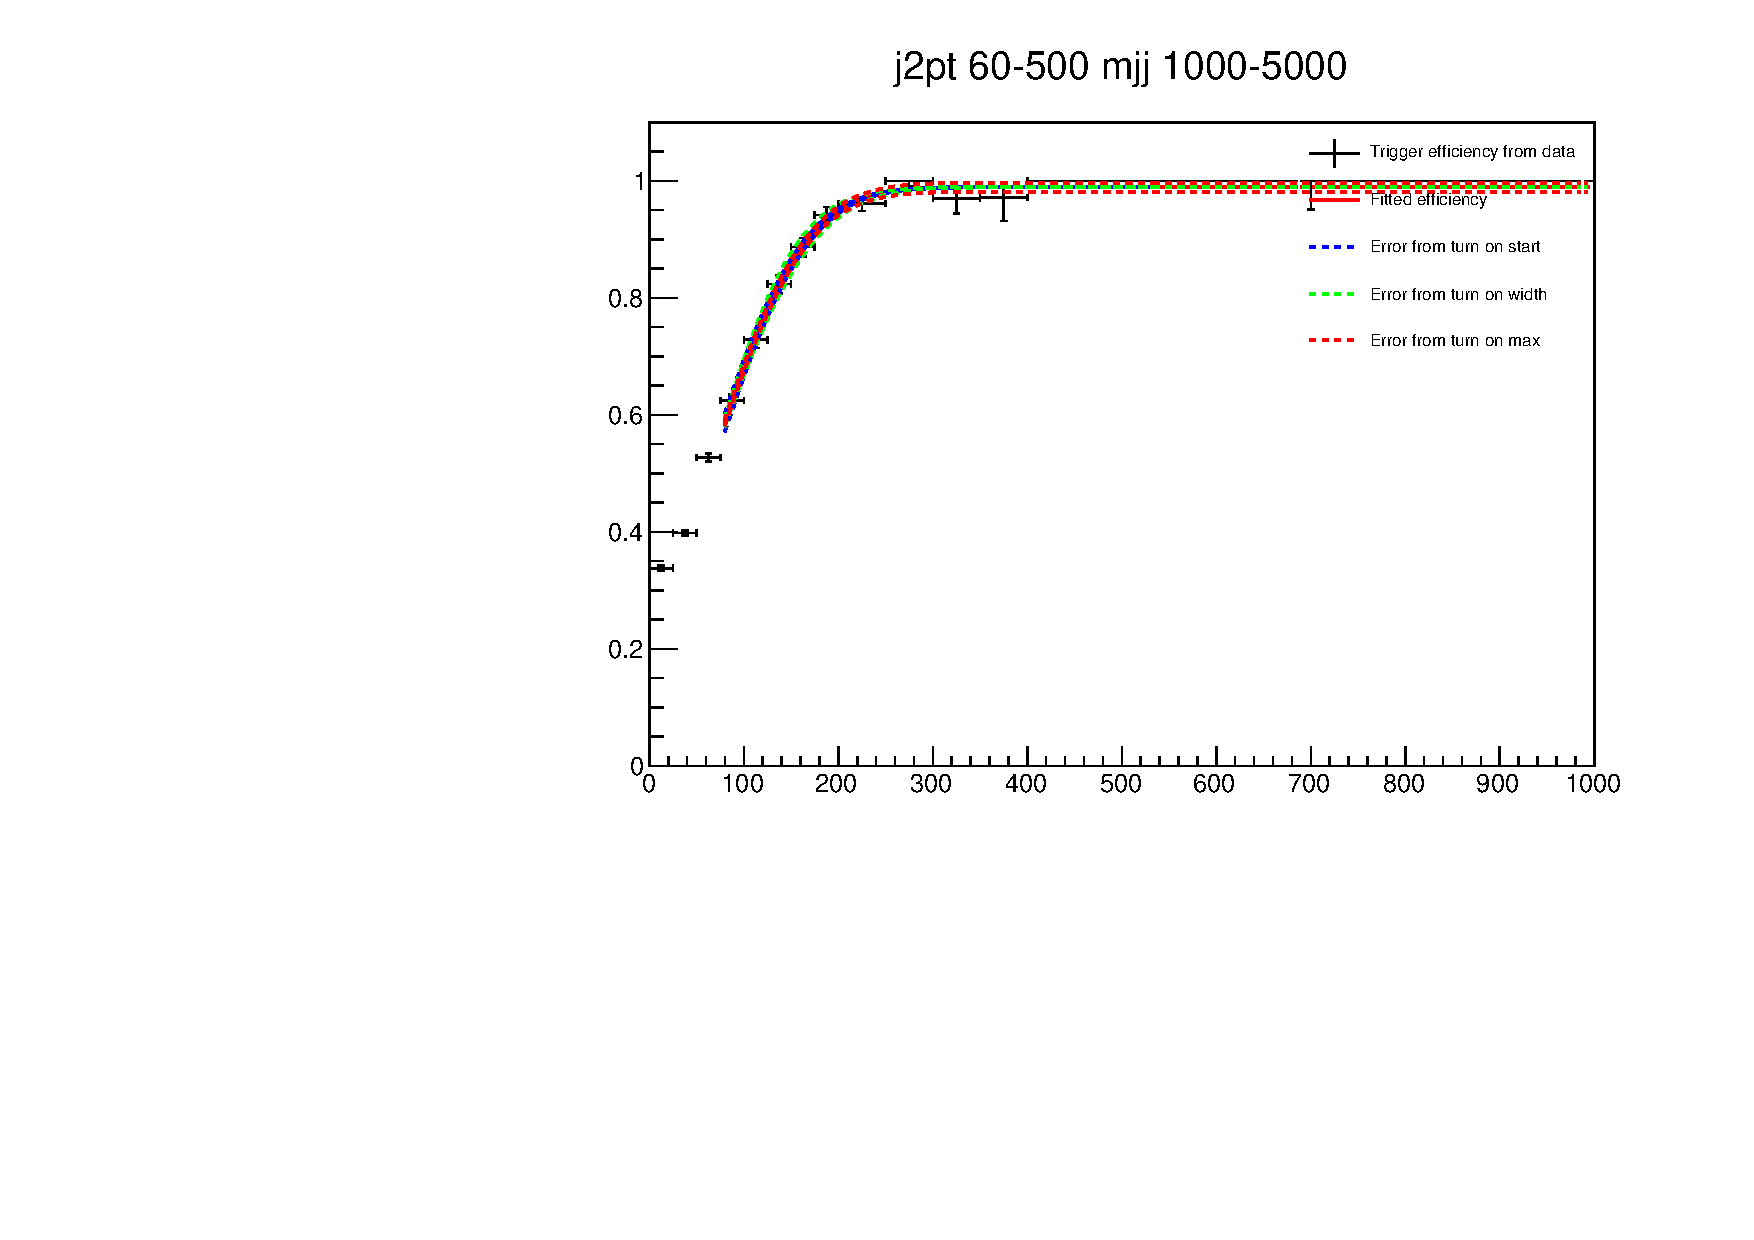
\includegraphics[width=\textwidth]{TalkPics/contplotsandpresel220914/trigfitplots/hData_MET_1D_45D.pdf}
    \end{block}
    \column{.5\textwidth}
    \begin{block}{Not so good}
      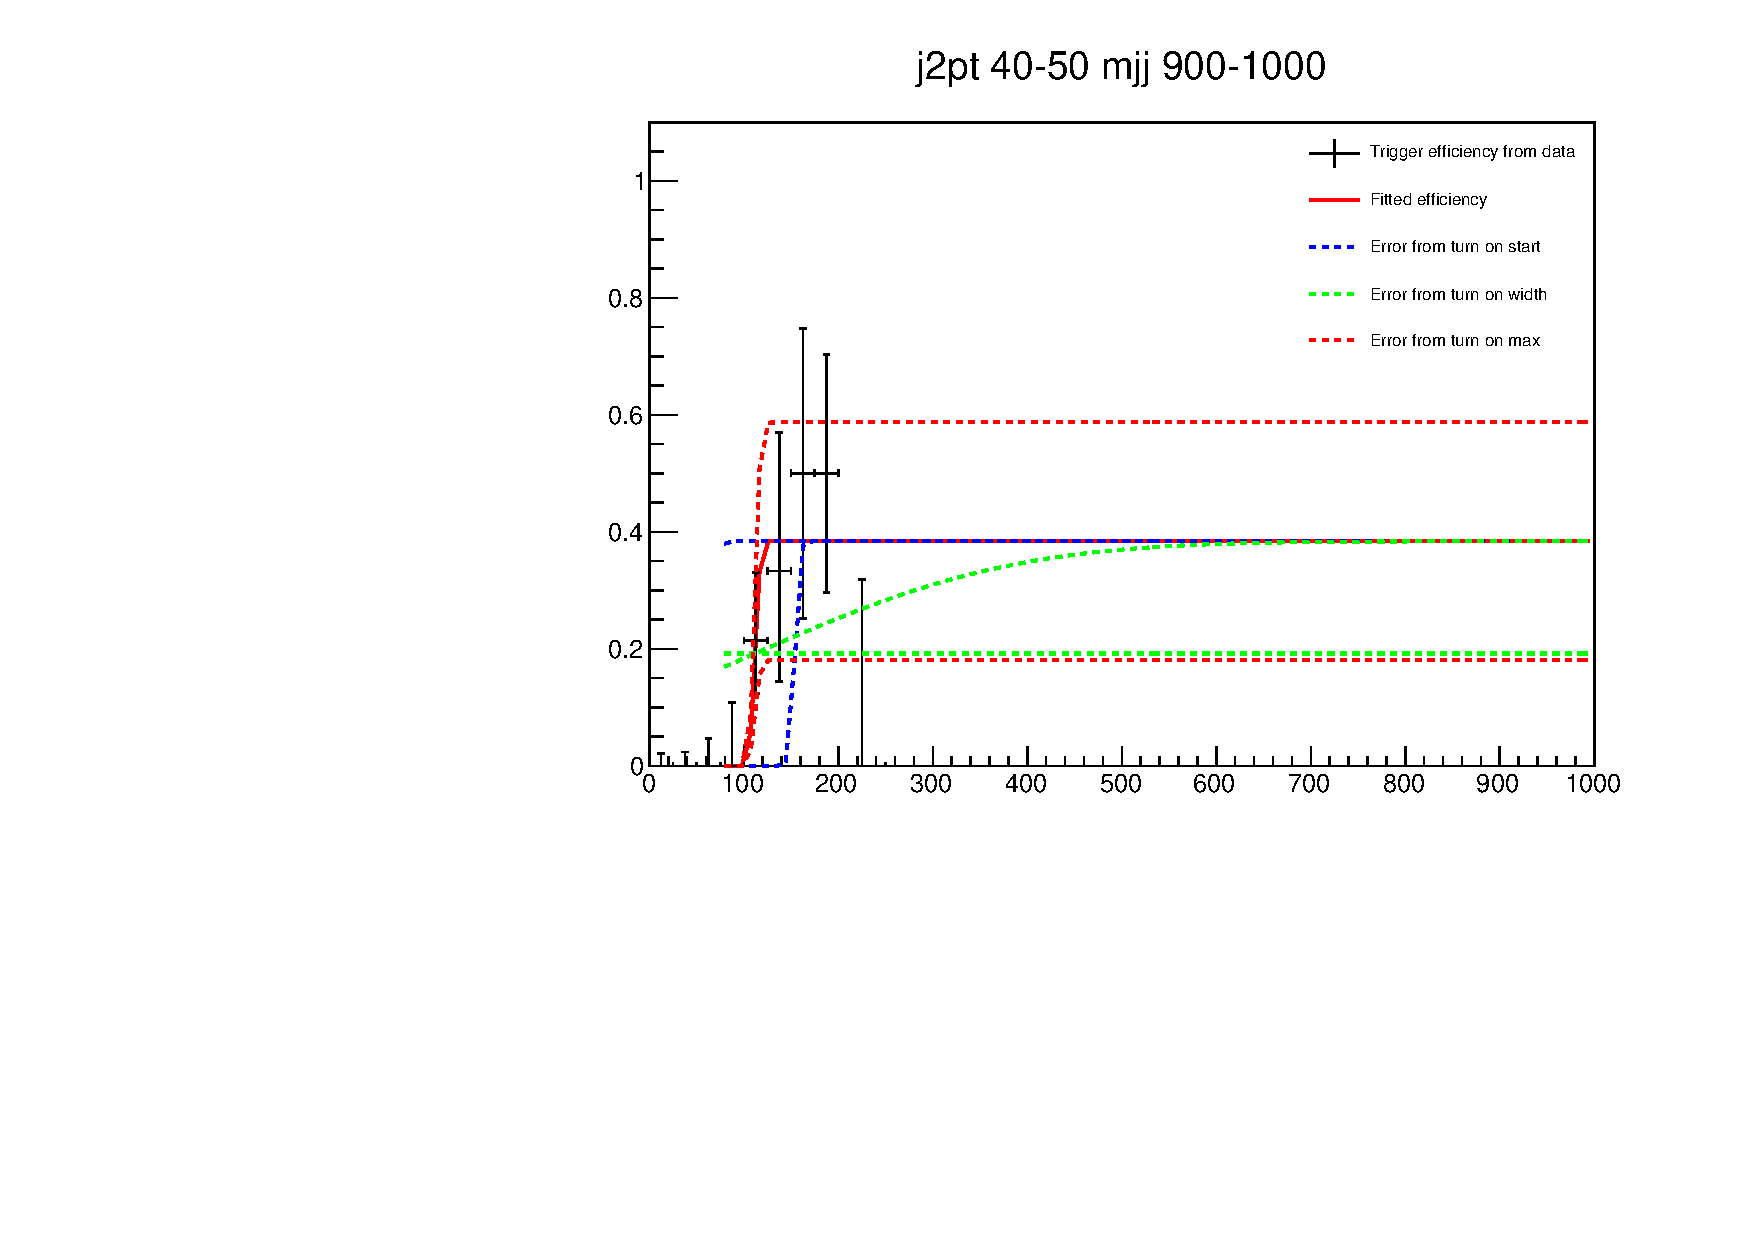
\includegraphics[width=\textwidth]{TalkPics/contplotsandpresel220914/trigfitplots/hData_MET_1D_24A.pdf}
    \end{block}
    
  \end{columns}
  \begin{block}{}
    \scriptsize
    \begin{itemize}
    \item Most fits look good
    \item A few bins have issues with numbers of events
    \item Some of the bins seem to slightly underestimate efficiency in the plateau
      \end{itemize}
  \end{block}
\end{frame}

%COMPARE CONT PLOTS BEFORE WITH PLOTS AFTER
%j2pt, met and mjj plots in regions where change is most obvious
\begin{frame}
  \frametitle{Control plots - munu}
  \begin{columns}
    \column{.5\textwidth}
    \begin{block}{Jet 2 pt - 1D trig weights}
      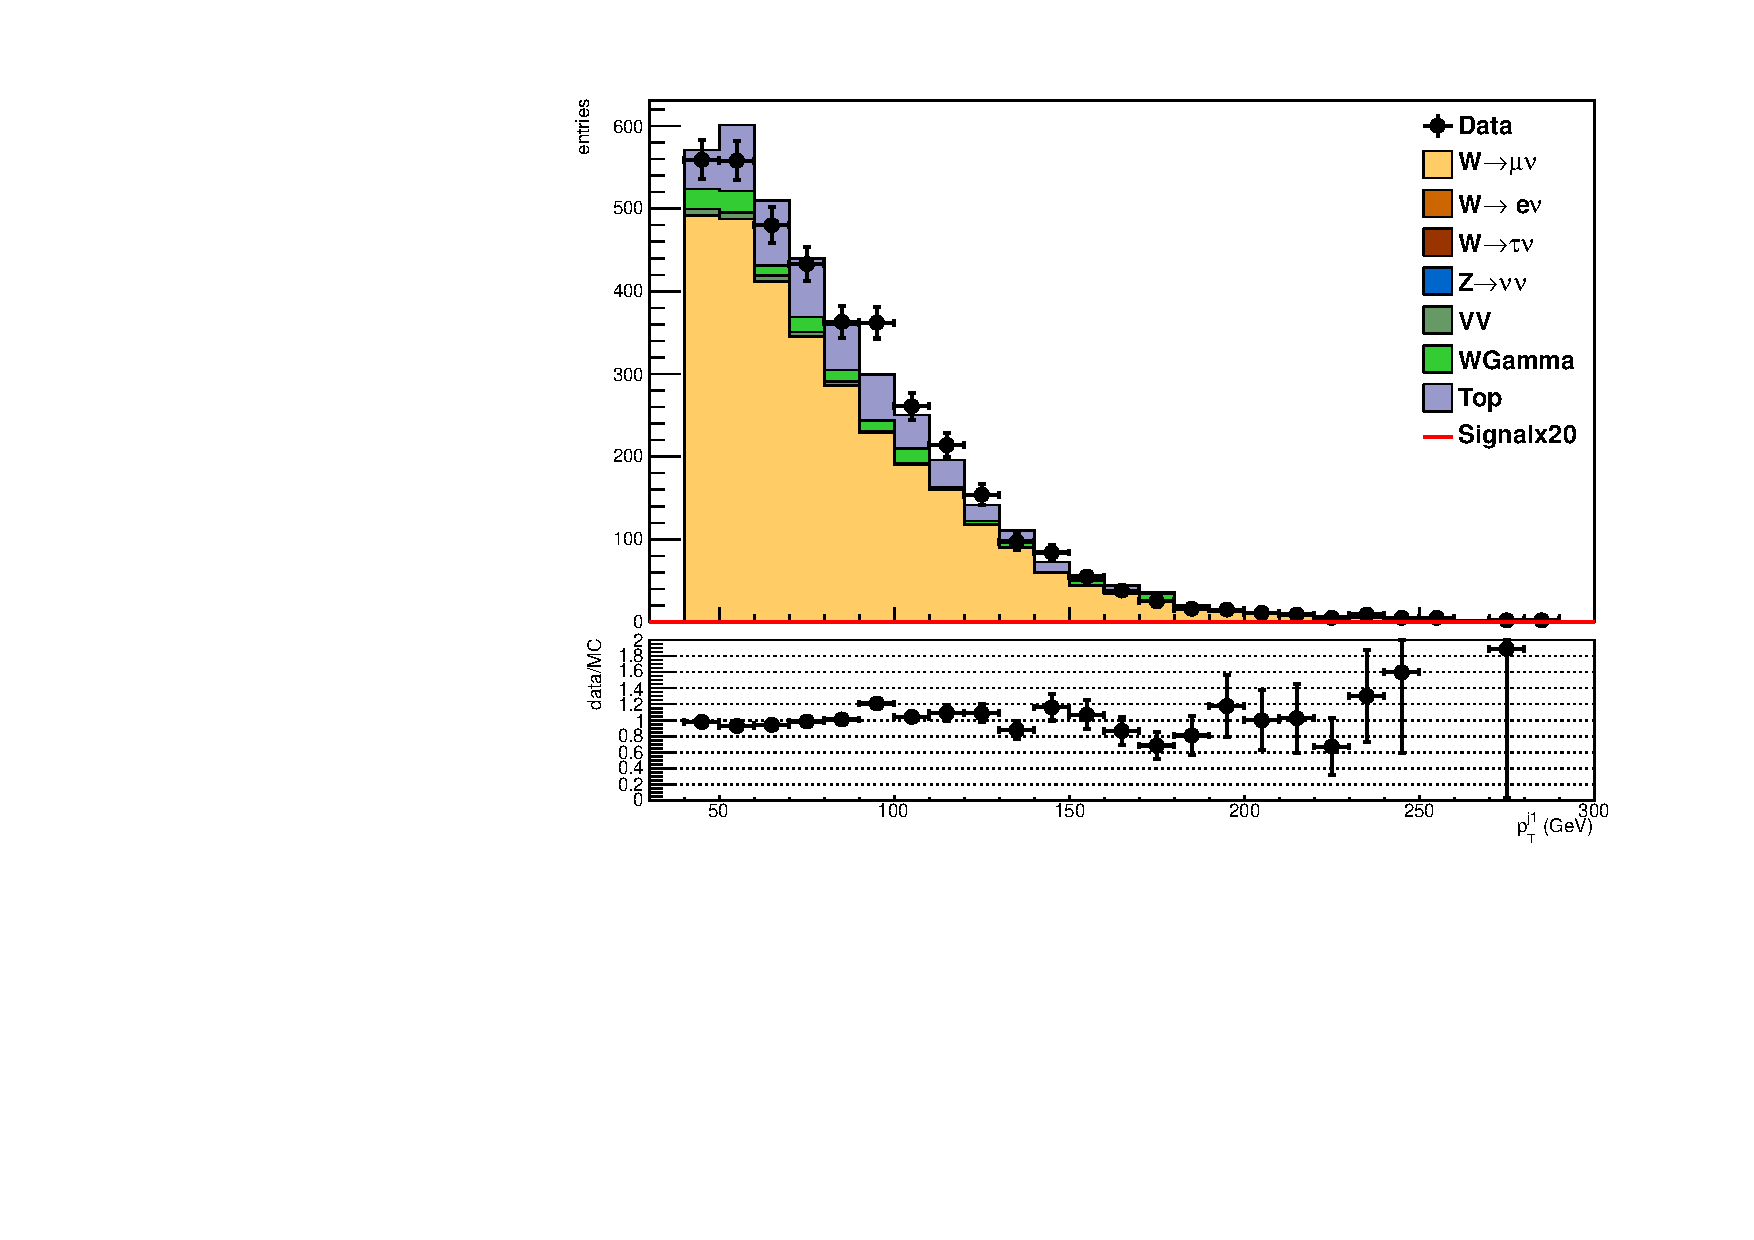
\includegraphics[width=\textwidth]{TalkPics/contplotsandpresel160914/output_contplots_alljets10lepweightfixed/munu_jet2_pt.pdf}
    \end{block}
    \column{.5\textwidth}
    \begin{block}{Jet 2 pt - 2D trig weights}
      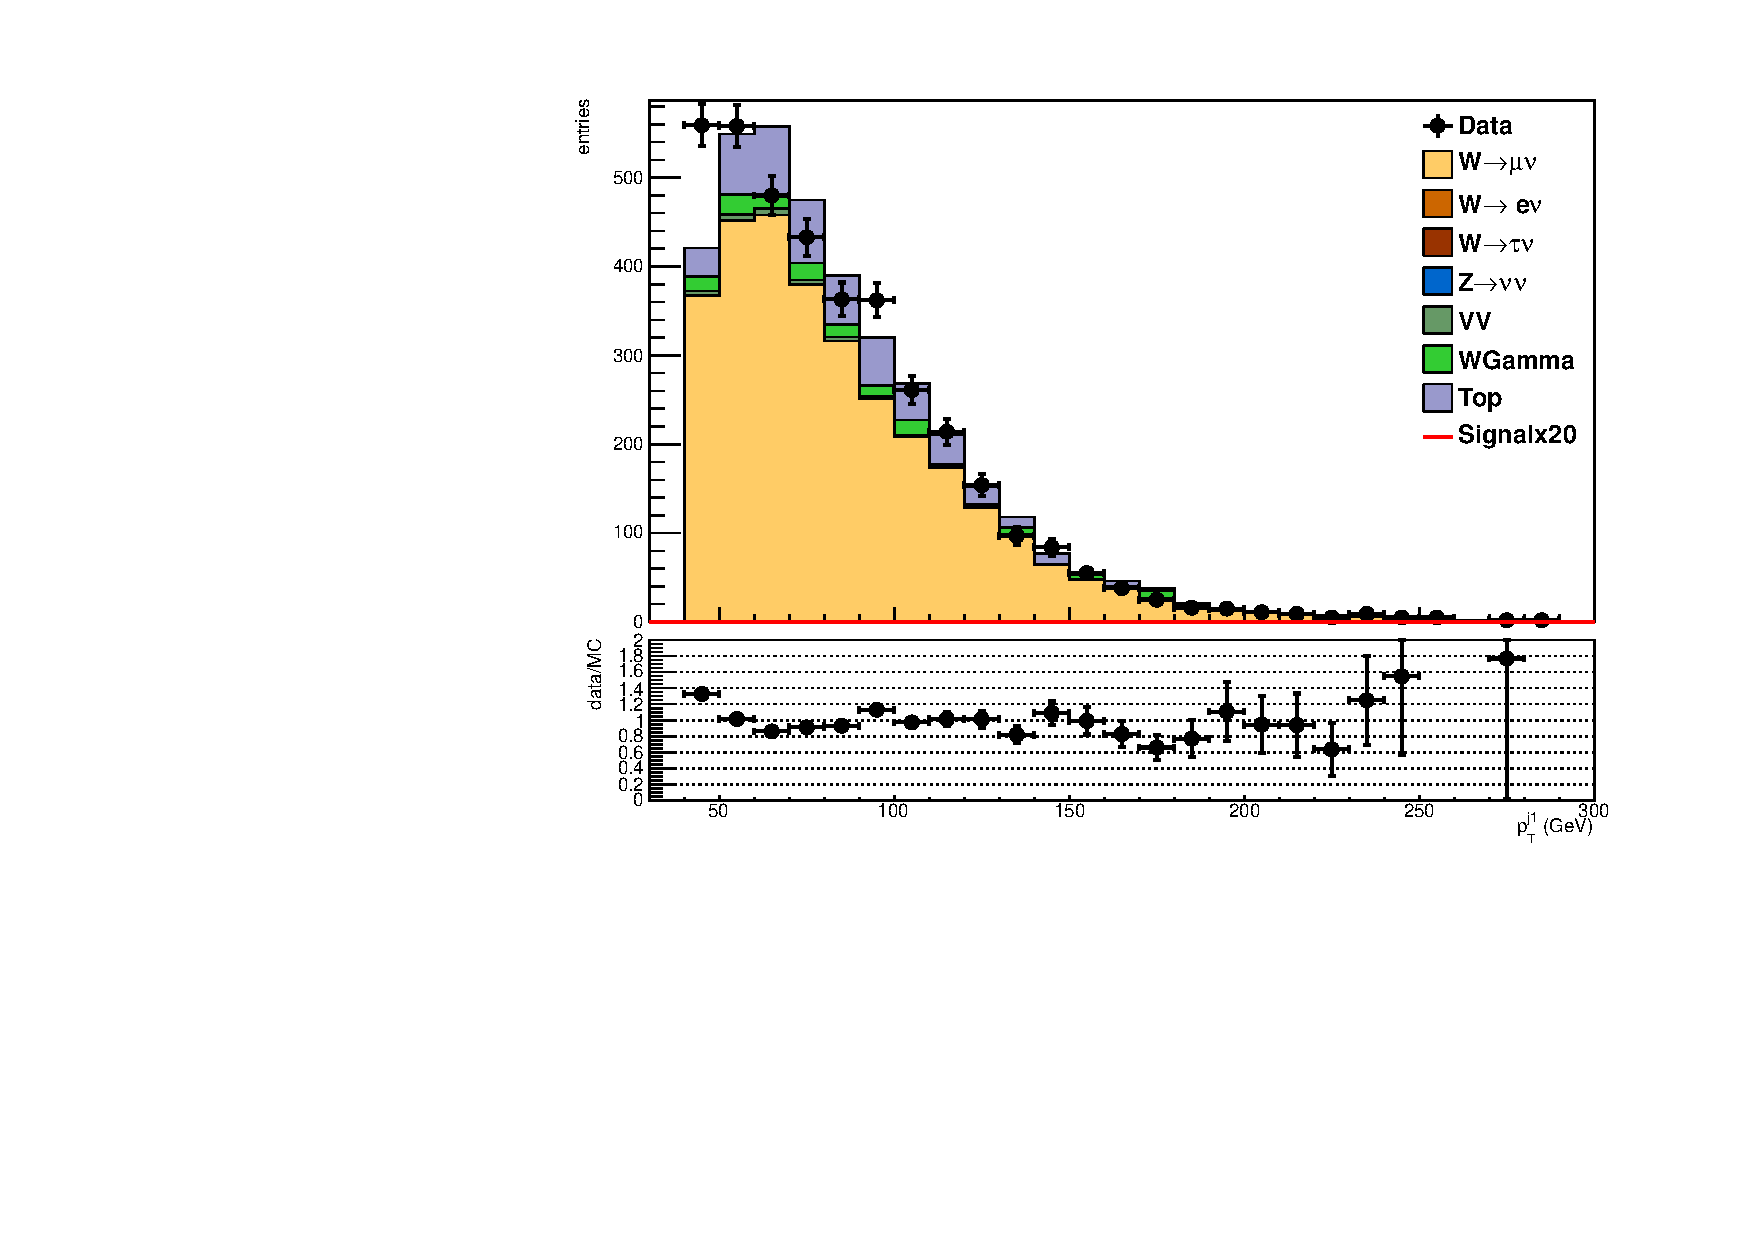
\includegraphics[width=\textwidth]{TalkPics/contplotsandpresel220914/output_contplots_rebinned2dweights/munu_jet2_pt.pdf}
    \end{block}

  \end{columns}
\end{frame}

\begin{frame}
  \frametitle{Control plots - munu}
  \begin{columns}
    \column{.5\textwidth}
    \begin{block}{Mjj - 1D trig weights}
      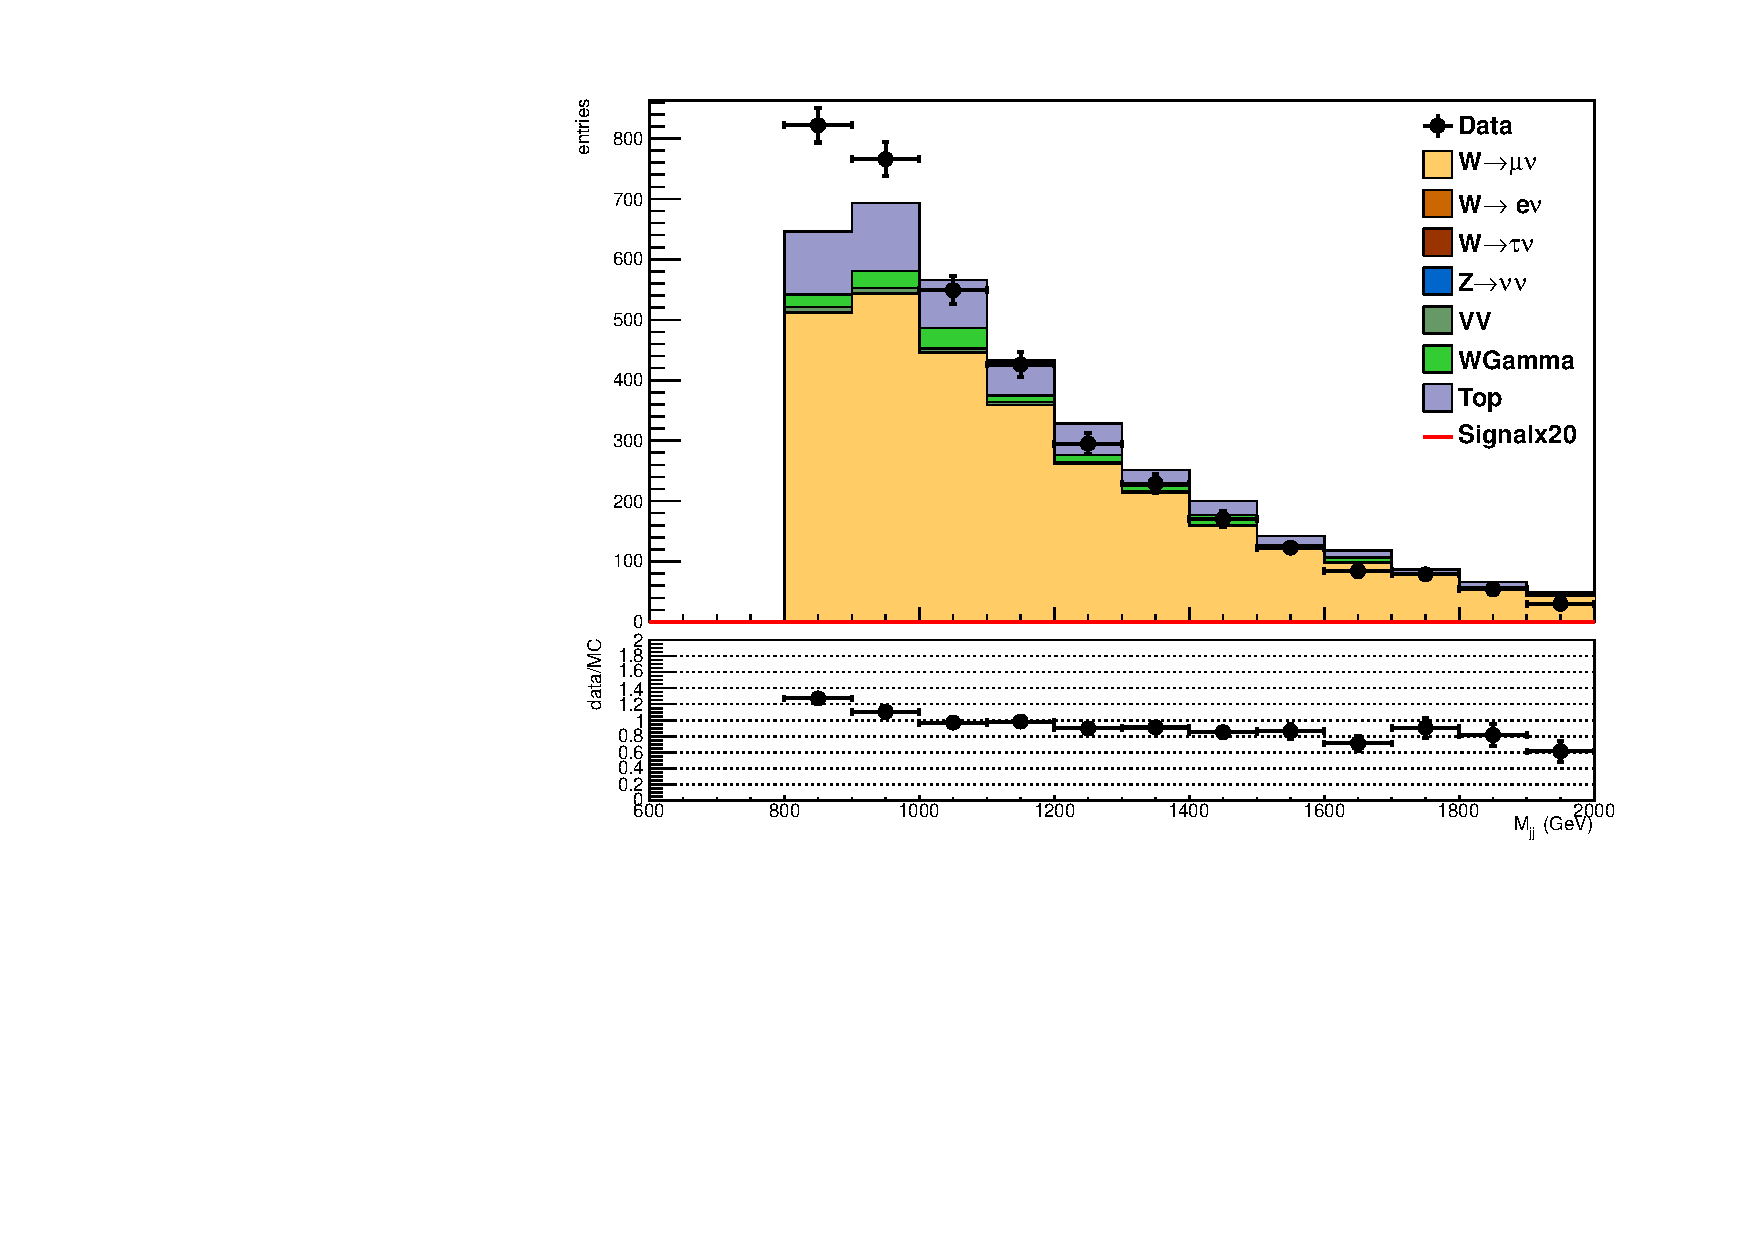
\includegraphics[width=\textwidth]{TalkPics/contplotsandpresel160914/output_contplots_alljets10lepweightfixed/munu_dijet_M.pdf}
    \end{block}
    \column{.5\textwidth}
    \begin{block}{Mjj - 2D trig weights}
      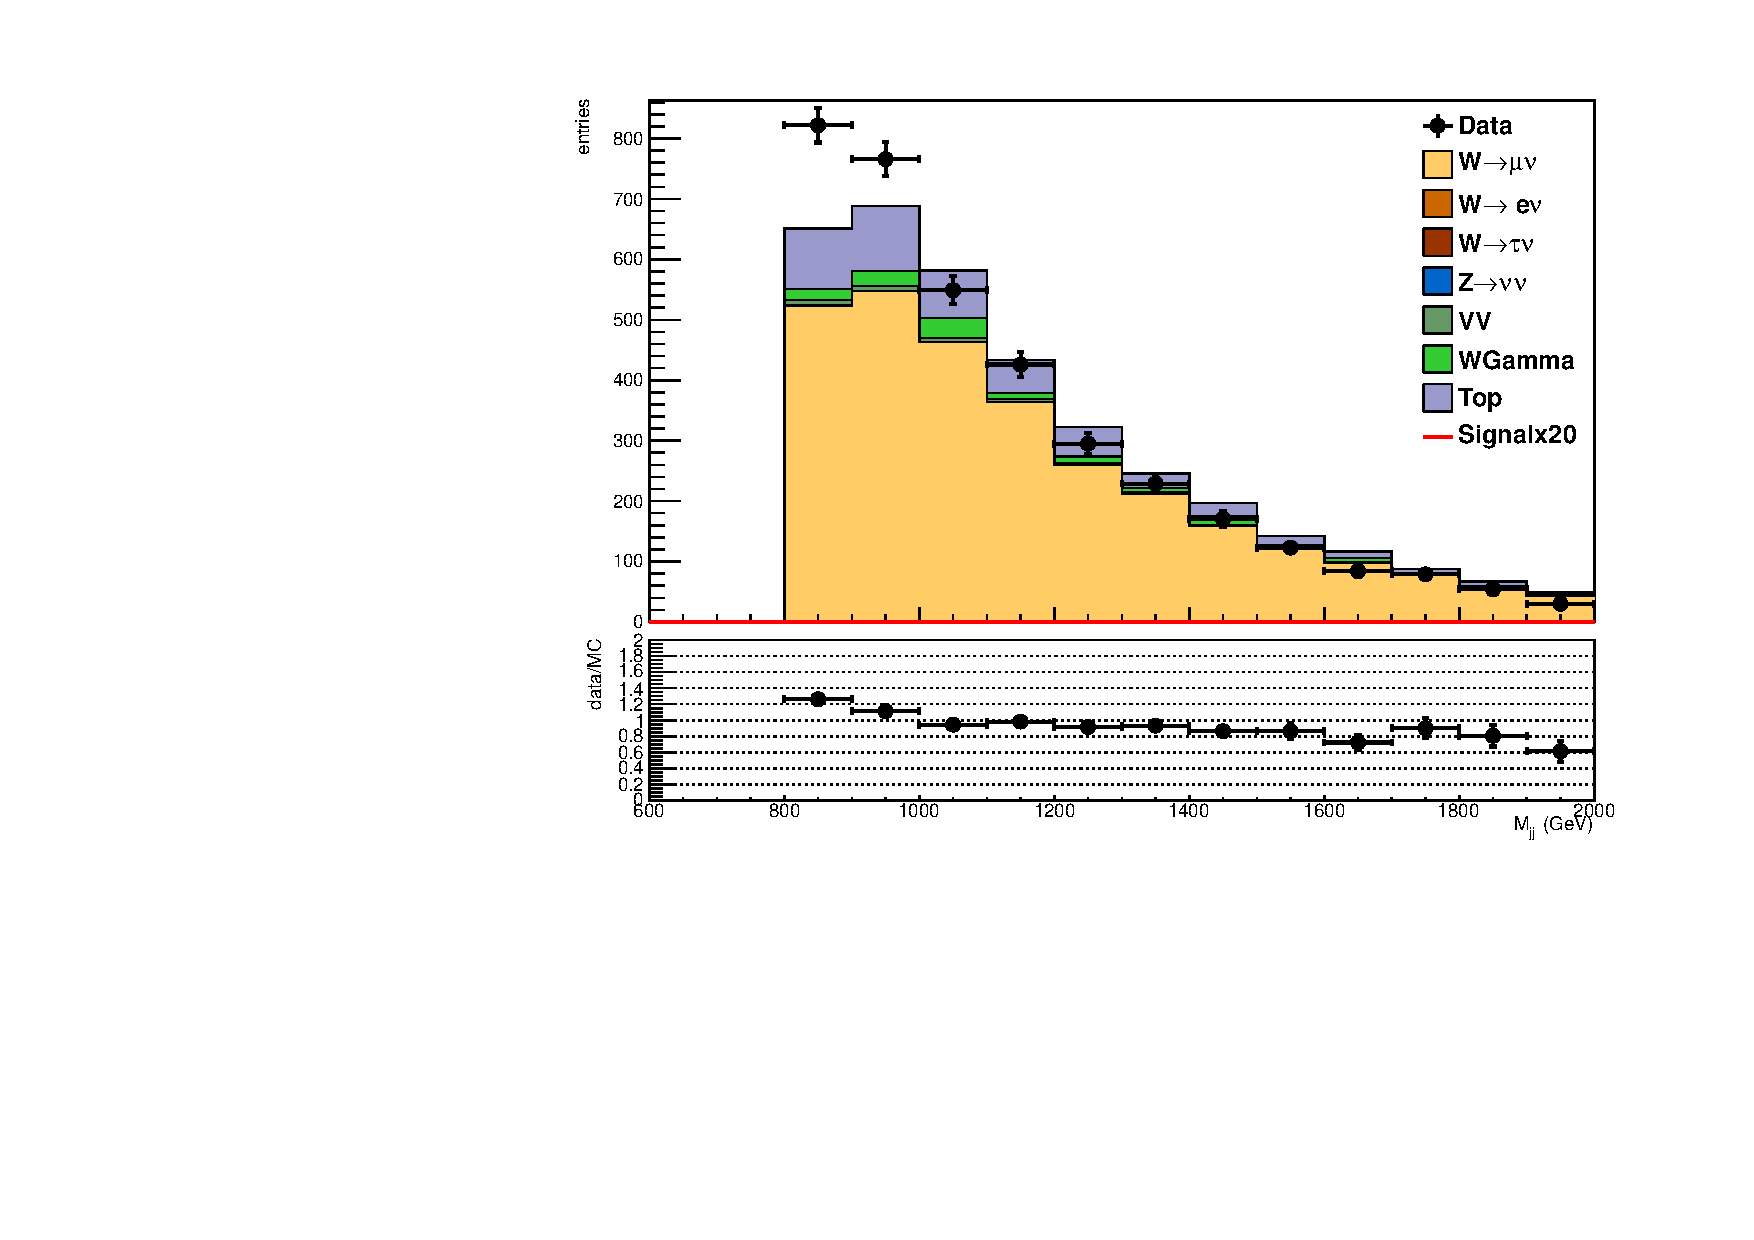
\includegraphics[width=\textwidth]{TalkPics/contplotsandpresel220914/output_contplots_rebinned2dweights/munu_dijet_M.pdf}
    \end{block}

  \end{columns}
\end{frame}

\begin{frame}
  \frametitle{Control plots - munu}
  \begin{columns}
    \column{.5\textwidth}
    \begin{block}{Metnomu - 1D trig weights}
      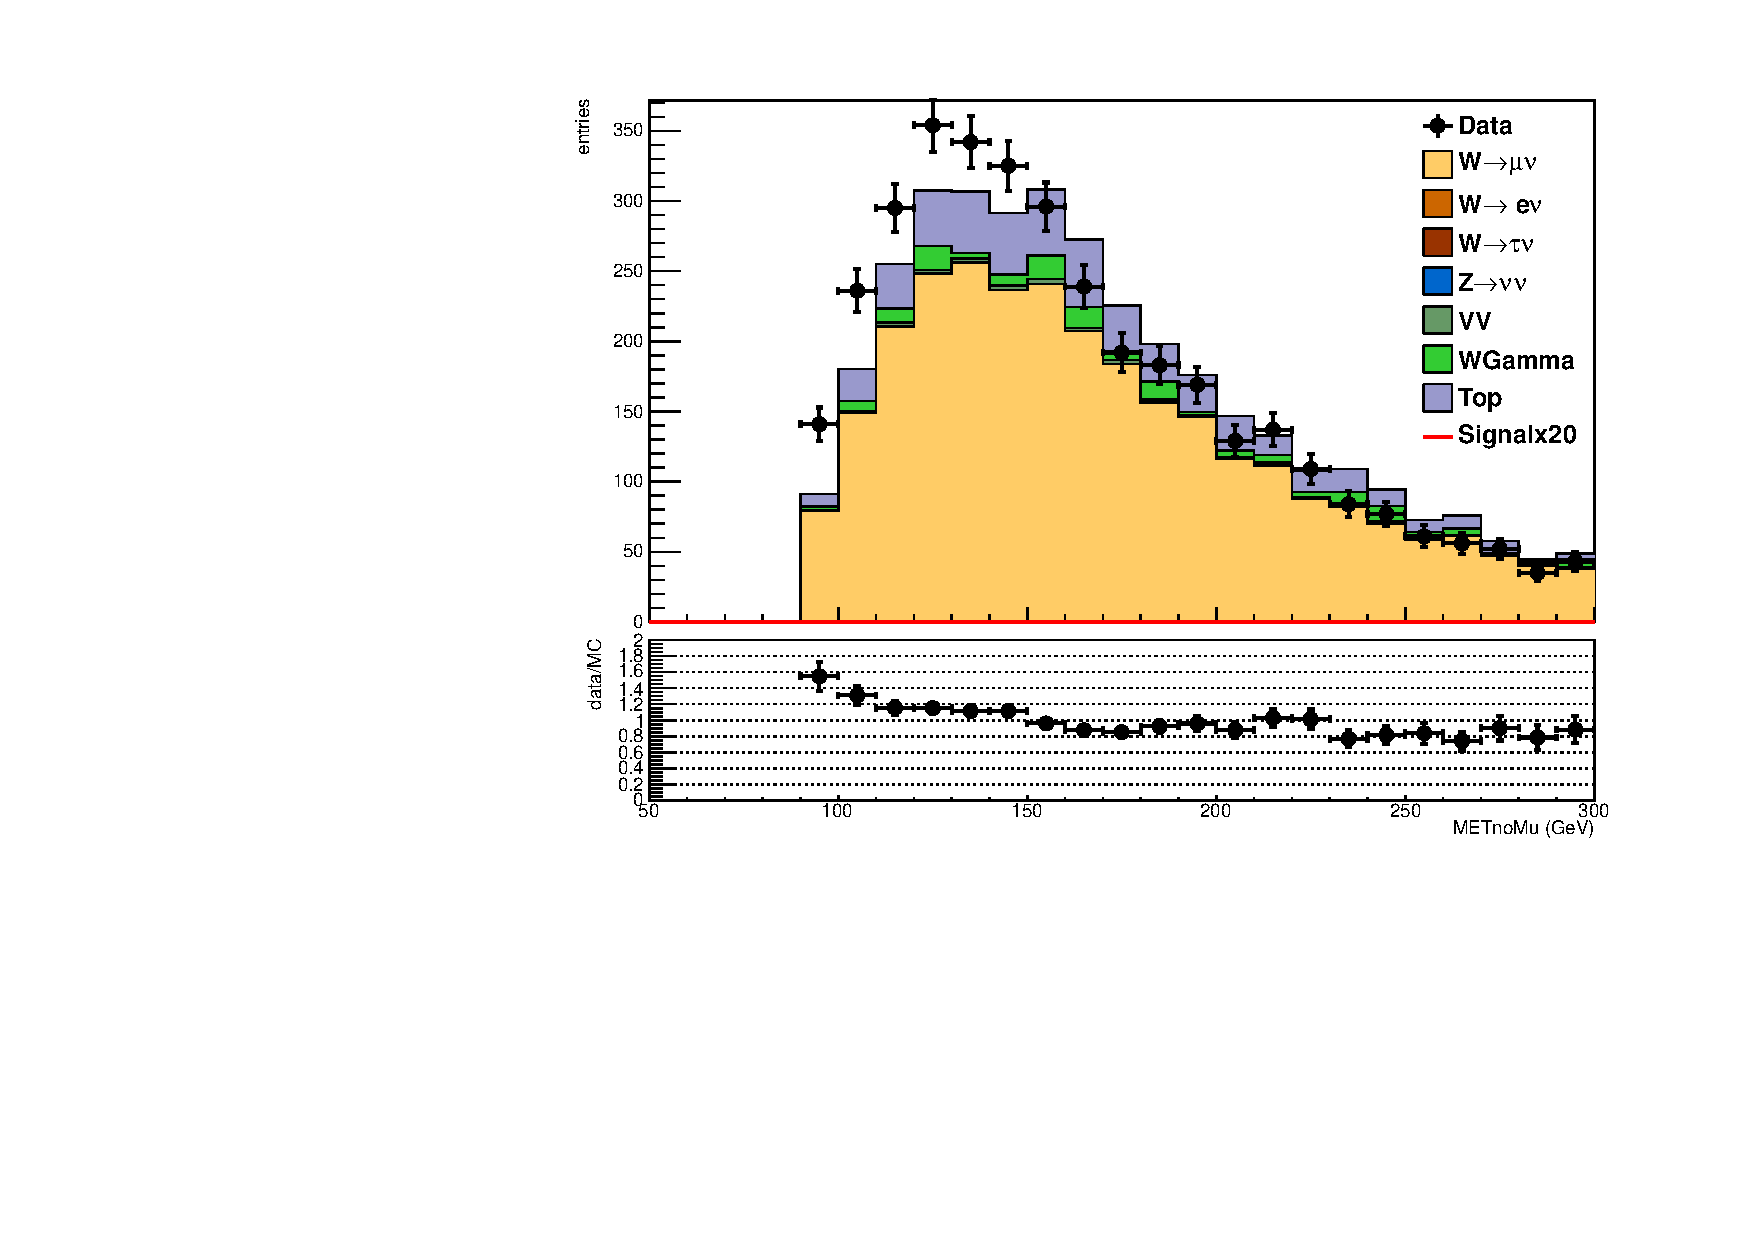
\includegraphics[width=\textwidth]{TalkPics/contplotsandpresel160914/output_contplots_alljets10lepweightfixed/munu_metnomuons.pdf}
    \end{block}
    \column{.5\textwidth}
    \begin{block}{Metnomu - 2D trig weights}
      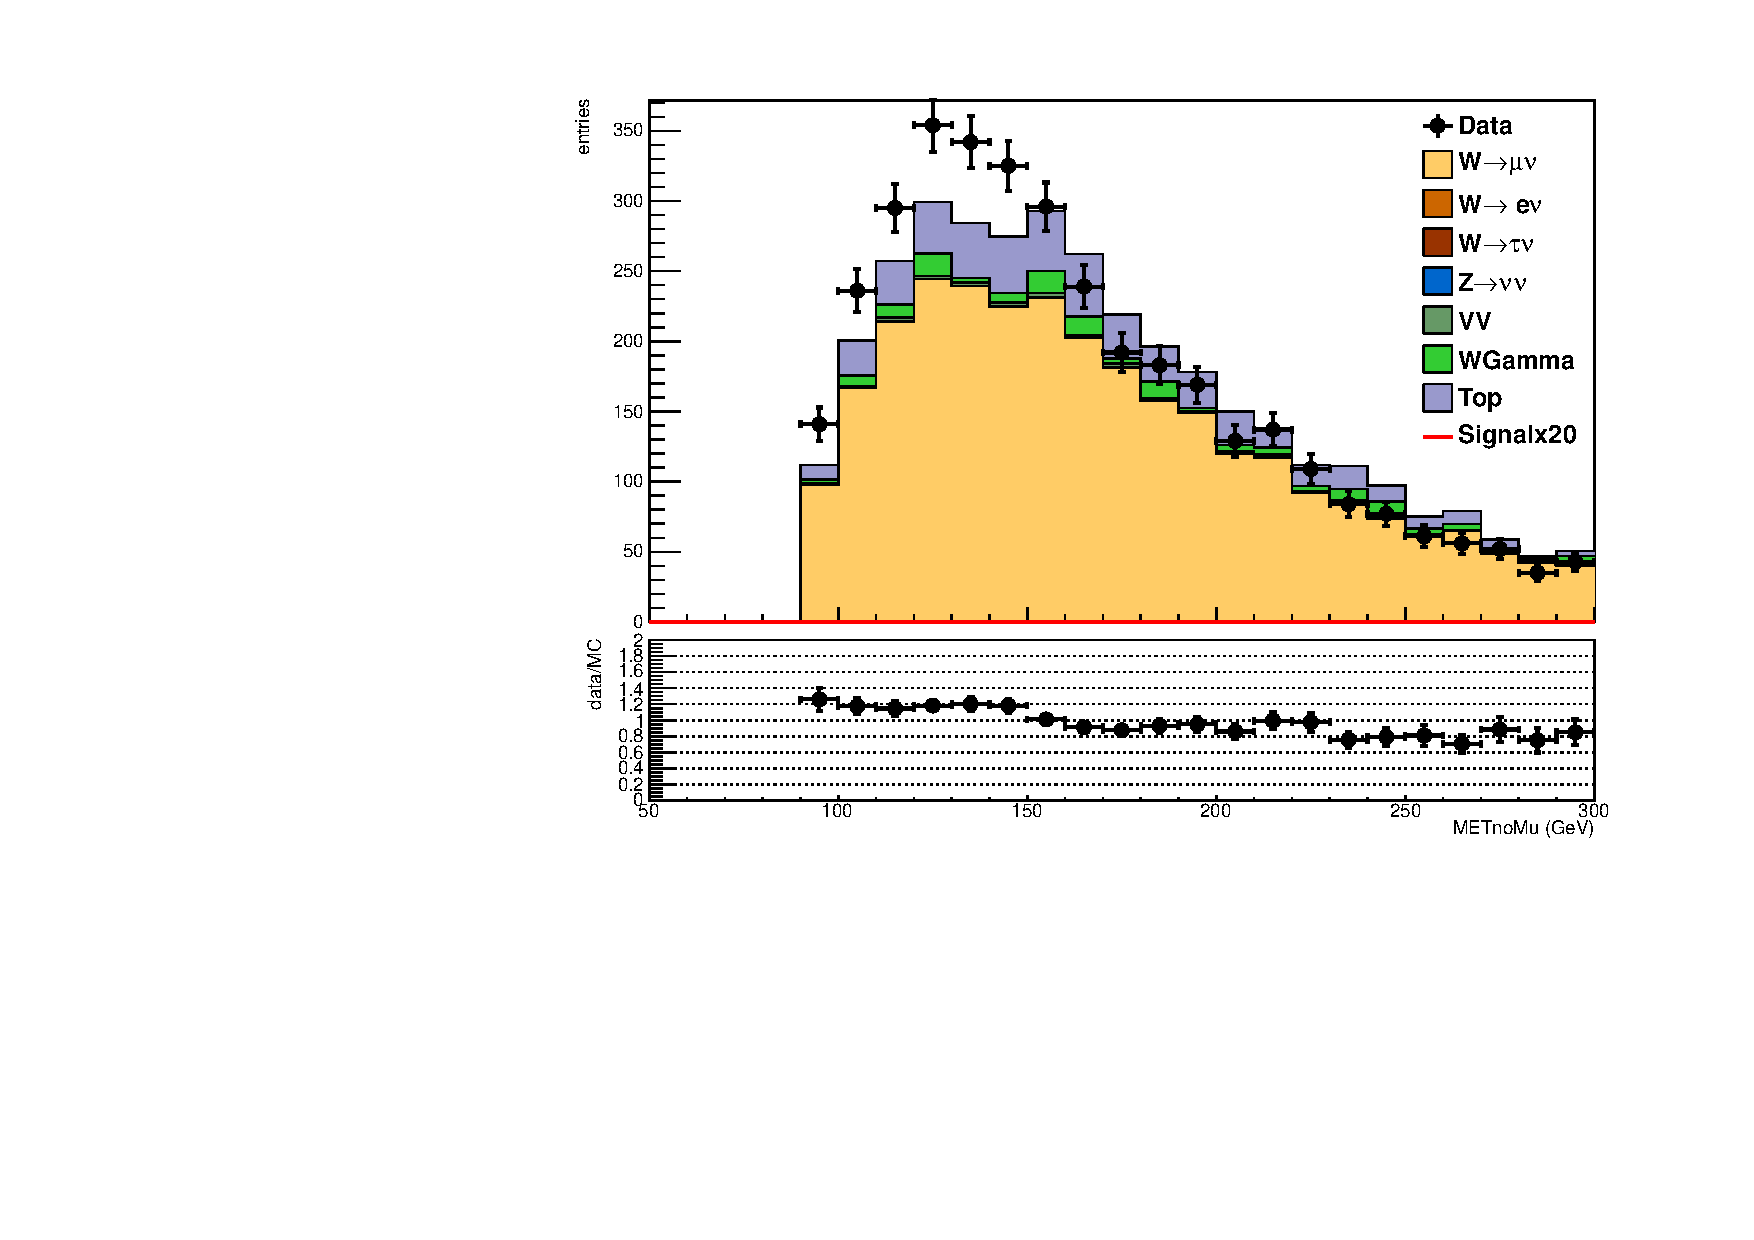
\includegraphics[width=\textwidth]{TalkPics/contplotsandpresel220914/output_contplots_rebinned2dweights/munu_metnomuons.pdf}
    \end{block}
  \end{columns}
  \begin{block}{}
    \scriptsize
    \begin{itemize}
    \item Possible step visible at 150 GeV
    \item[-] This is a bin boundary in the new trigger weights
    \end{itemize}
  \end{block}
\end{frame}

\begin{frame}
  \frametitle{New Trigger Weight Summary}
  \begin{block}{}
    \scriptsize
    \begin{itemize}
    \item New trigger weights improve met agreement and slightly degrade jet 2 pt agreement
    \item Other distributions appear relatively unchanged
    \item Now need to investigate other possibilities for munu disagreement
    \end{itemize}
  \end{block}
\end{frame}
%!!munu region plots which show increased QCD contribution
%!!mt cut in munu region

\begin{frame}
  \frametitle{Control plots - munu}
  \begin{columns}
    \column{.5\textwidth}
    \begin{block}{$m_{T}$}
      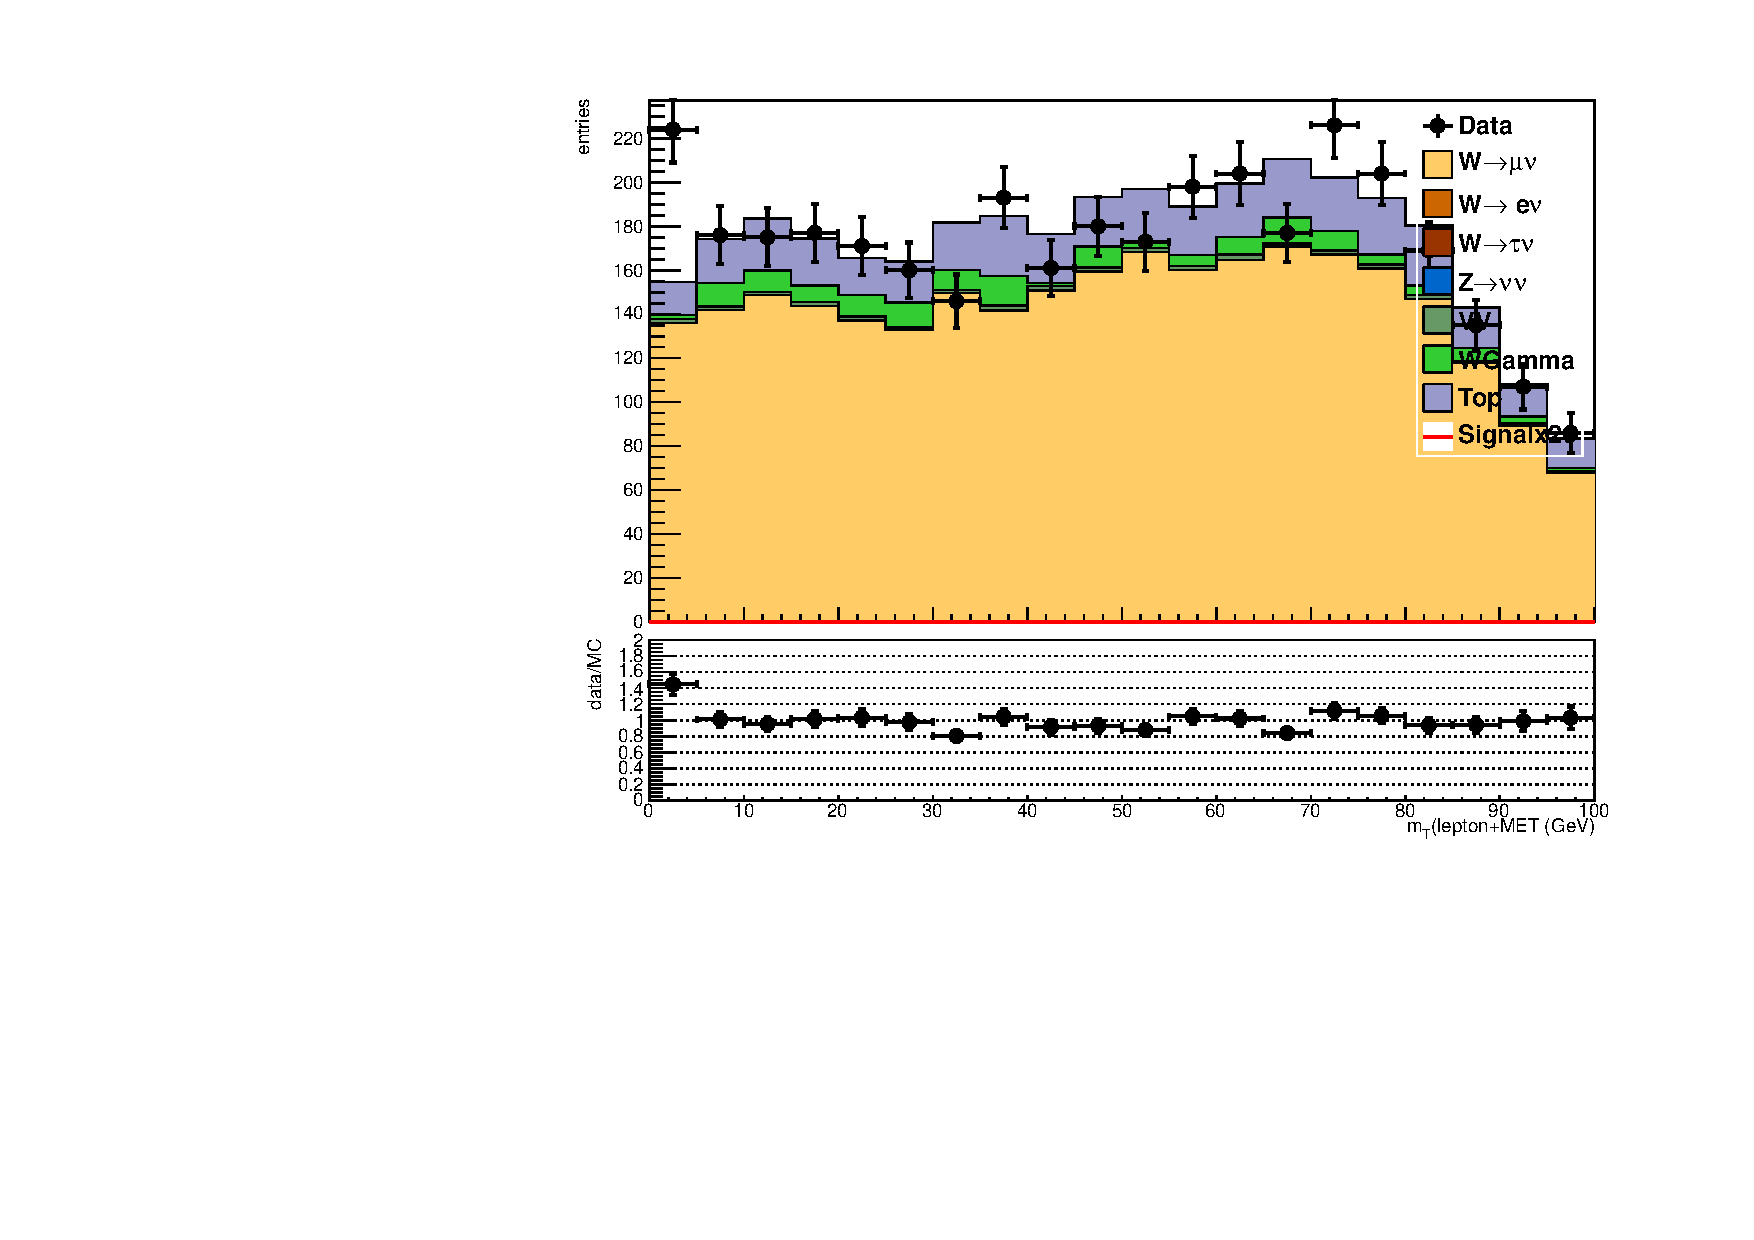
\includegraphics[width=\textwidth]{TalkPics/contplotsandpresel220914/output_contplots_rebinned2dweights/munu_lep_mt.pdf}
    \end{block}
    \column{.5\textwidth}
    \begin{block}{dijet-met pt fraction}
      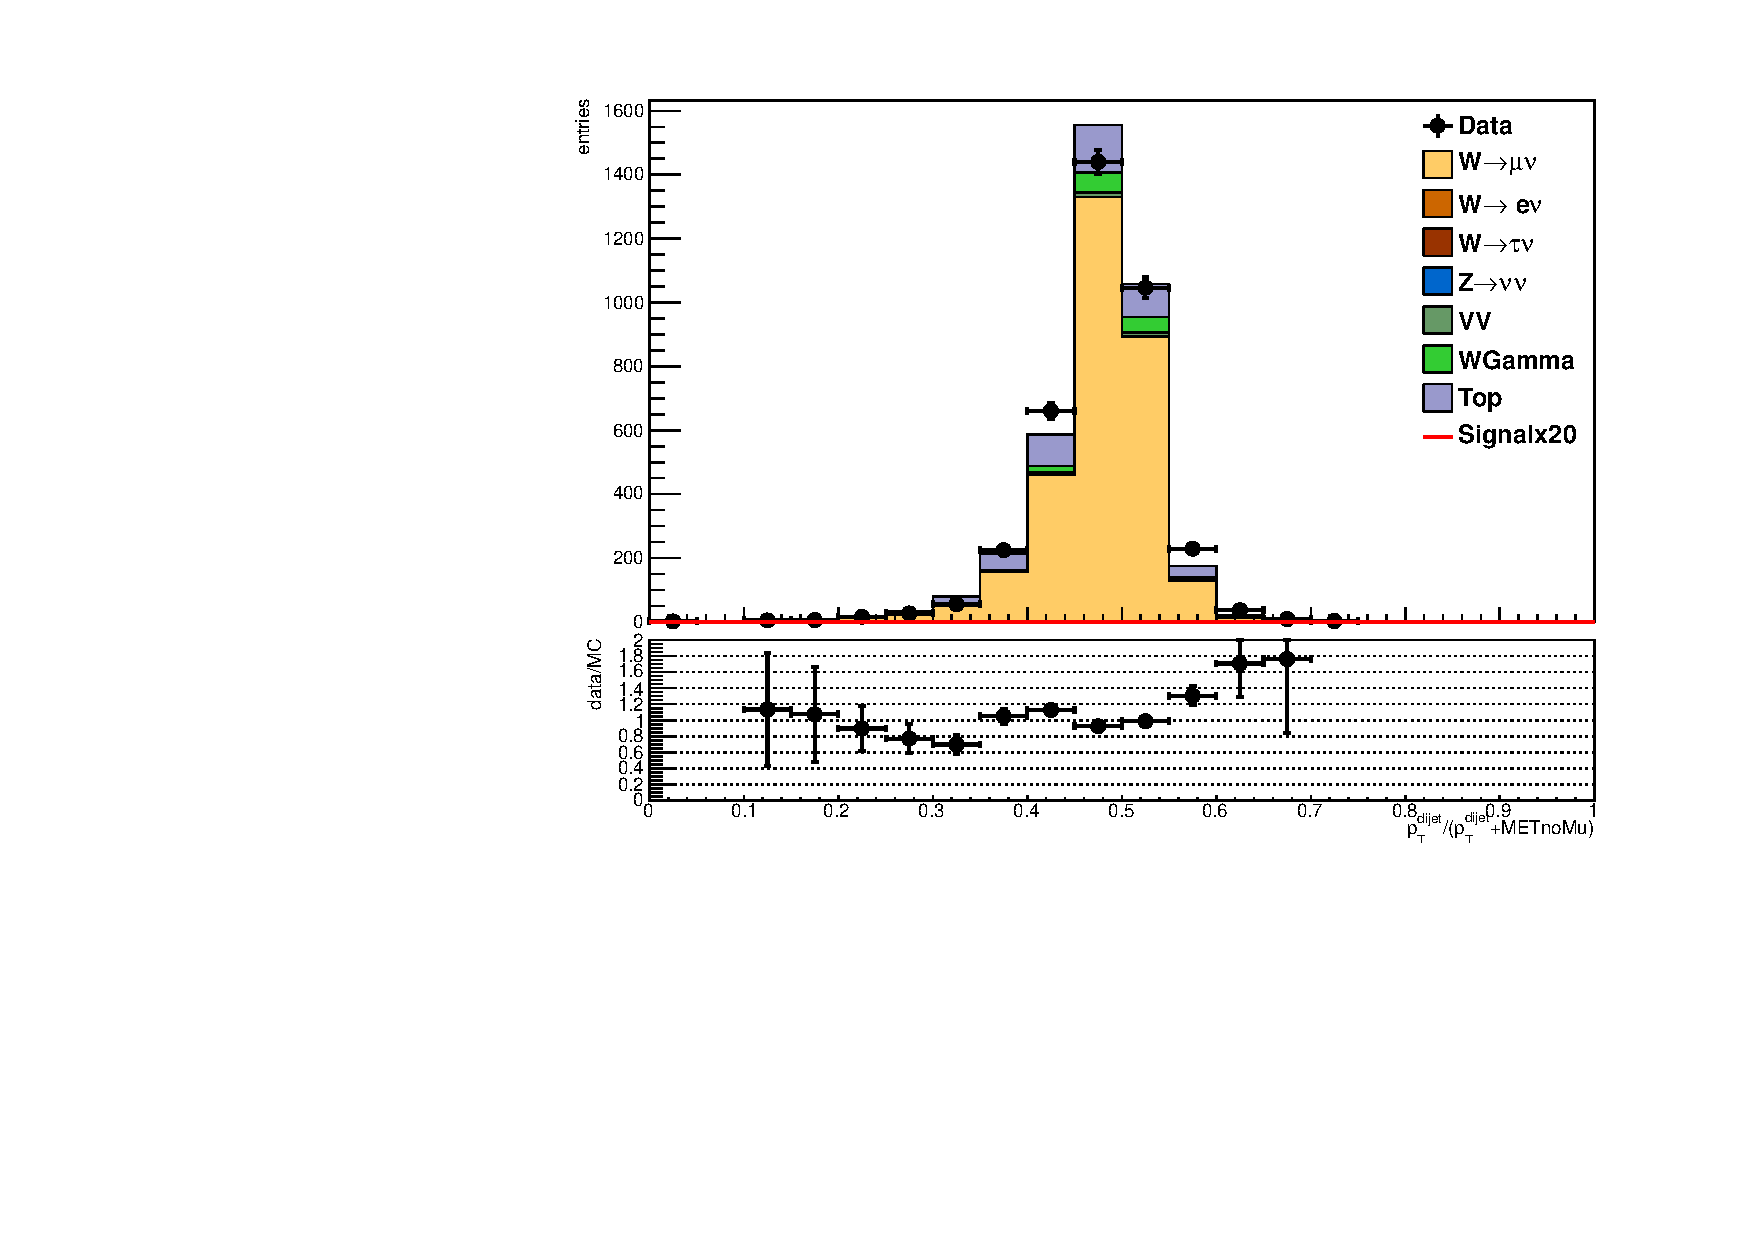
\includegraphics[width=\textwidth]{TalkPics/contplotsandpresel220914/output_contplots_rebinned2dweights/munu_dijetmetnomu_ptfraction.pdf}
    \end{block}
  \end{columns}
\end{frame}

\begin{frame}
  \frametitle{Control plots - munu}
  \begin{columns}
    \column{.5\textwidth}
    \begin{block}{metnomu significance}
      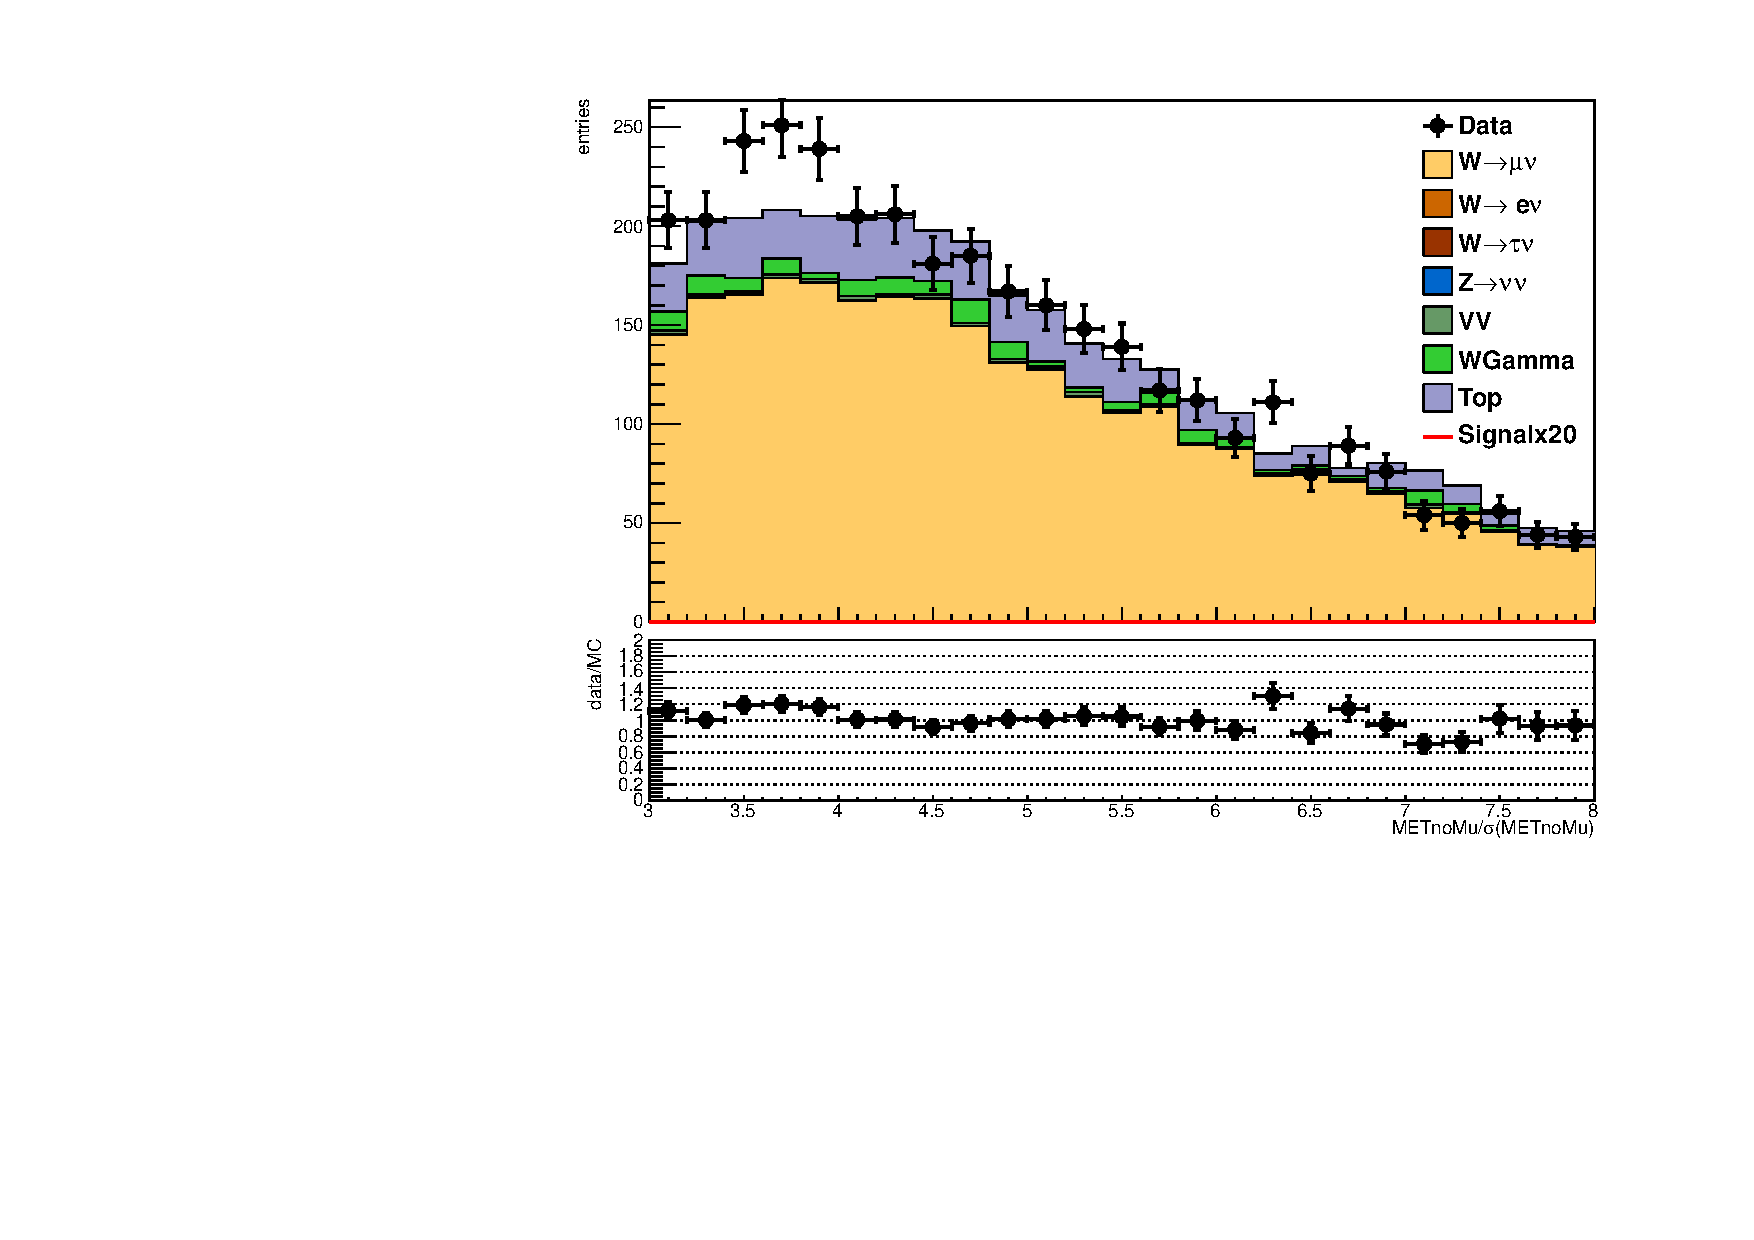
\includegraphics[width=\textwidth]{TalkPics/contplotsandpresel220914/output_contplots_rebinned2dweights/munu_metnomu_significance.pdf}
    \end{block}
    \column{.5\textwidth}
    \begin{block}{jet-met min $\Delta\phi$}
      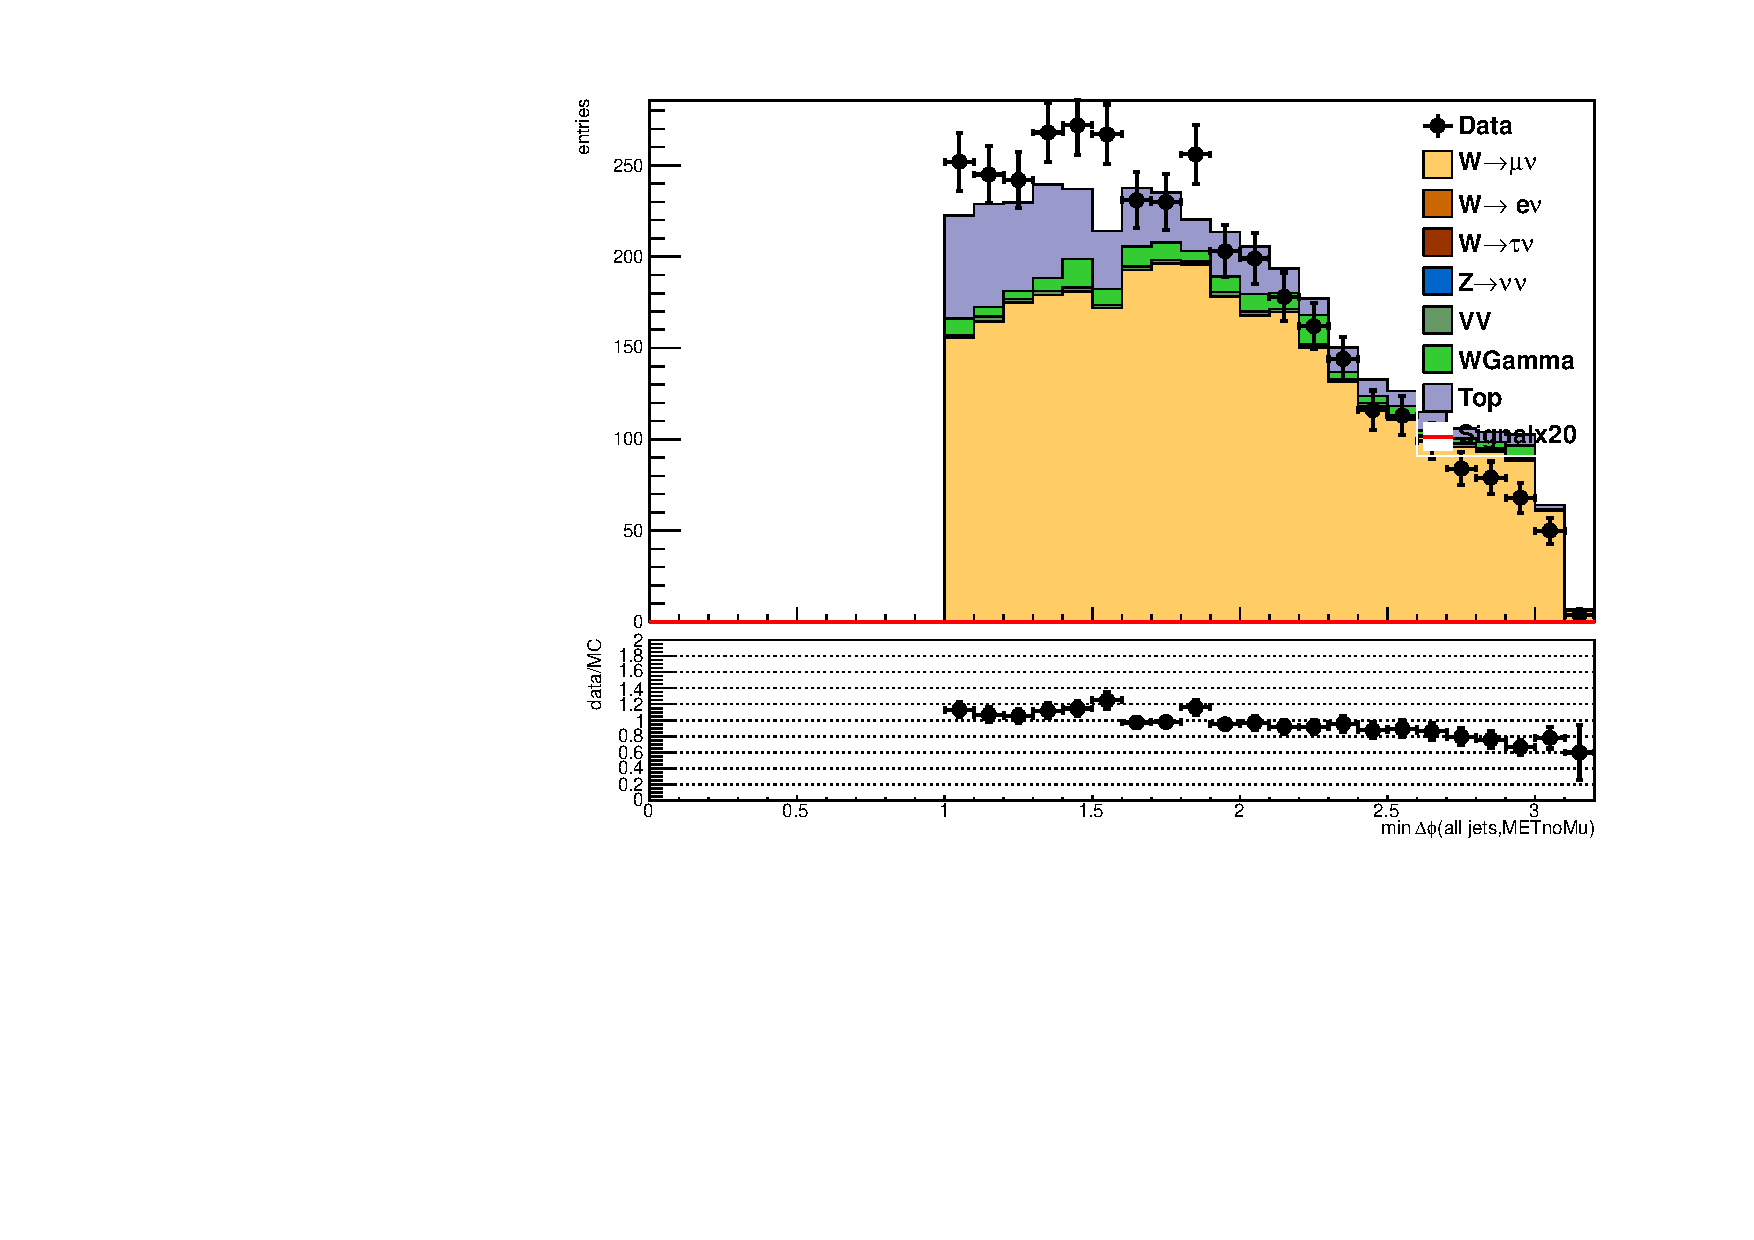
\includegraphics[width=\textwidth]{TalkPics/contplotsandpresel220914/output_contplots_rebinned2dweights/munu_alljetsmetnomu_mindphi.pdf}
    \end{block}
  \end{columns}
\end{frame}

\begin{frame}
  \frametitle{Try mt cut}
  \begin{block}{}
    \scriptsize
    \begin{itemize}
    \item All plots show MC deficit in QCD region
    \item Try a transverse mass cut of 10 GeV
    \end{itemize}
  \end{block}
  \begin{columns}
    \column{.5\textwidth}
    \begin{block}{\scriptsize metnomu significance - no mt cut}
      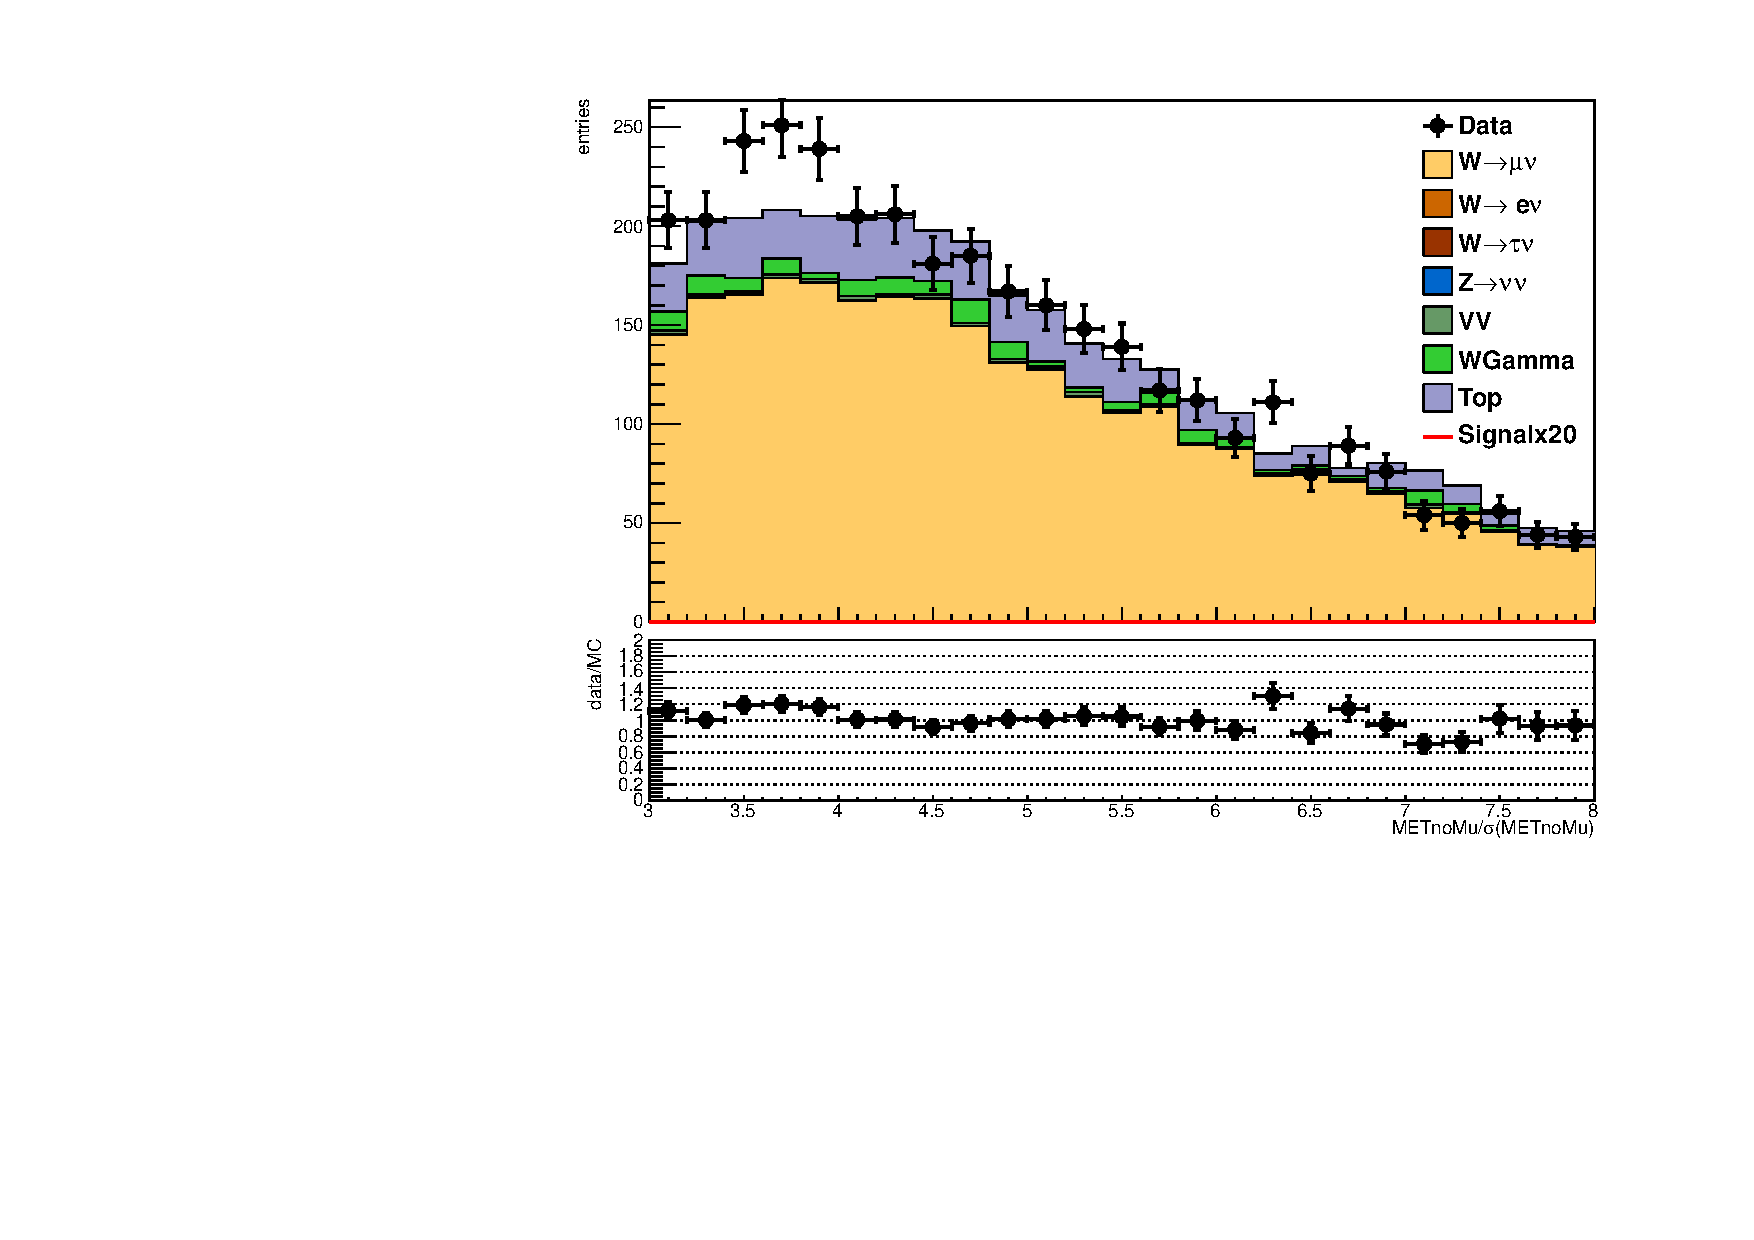
\includegraphics[width=\textwidth]{TalkPics/contplotsandpresel220914/output_contplots_rebinned2dweights/munu_metnomu_significance.pdf}
    \end{block}
    \column{.5\textwidth}
    \begin{block}{\scriptsize metnomu significance - mt$>10$ GeV}
      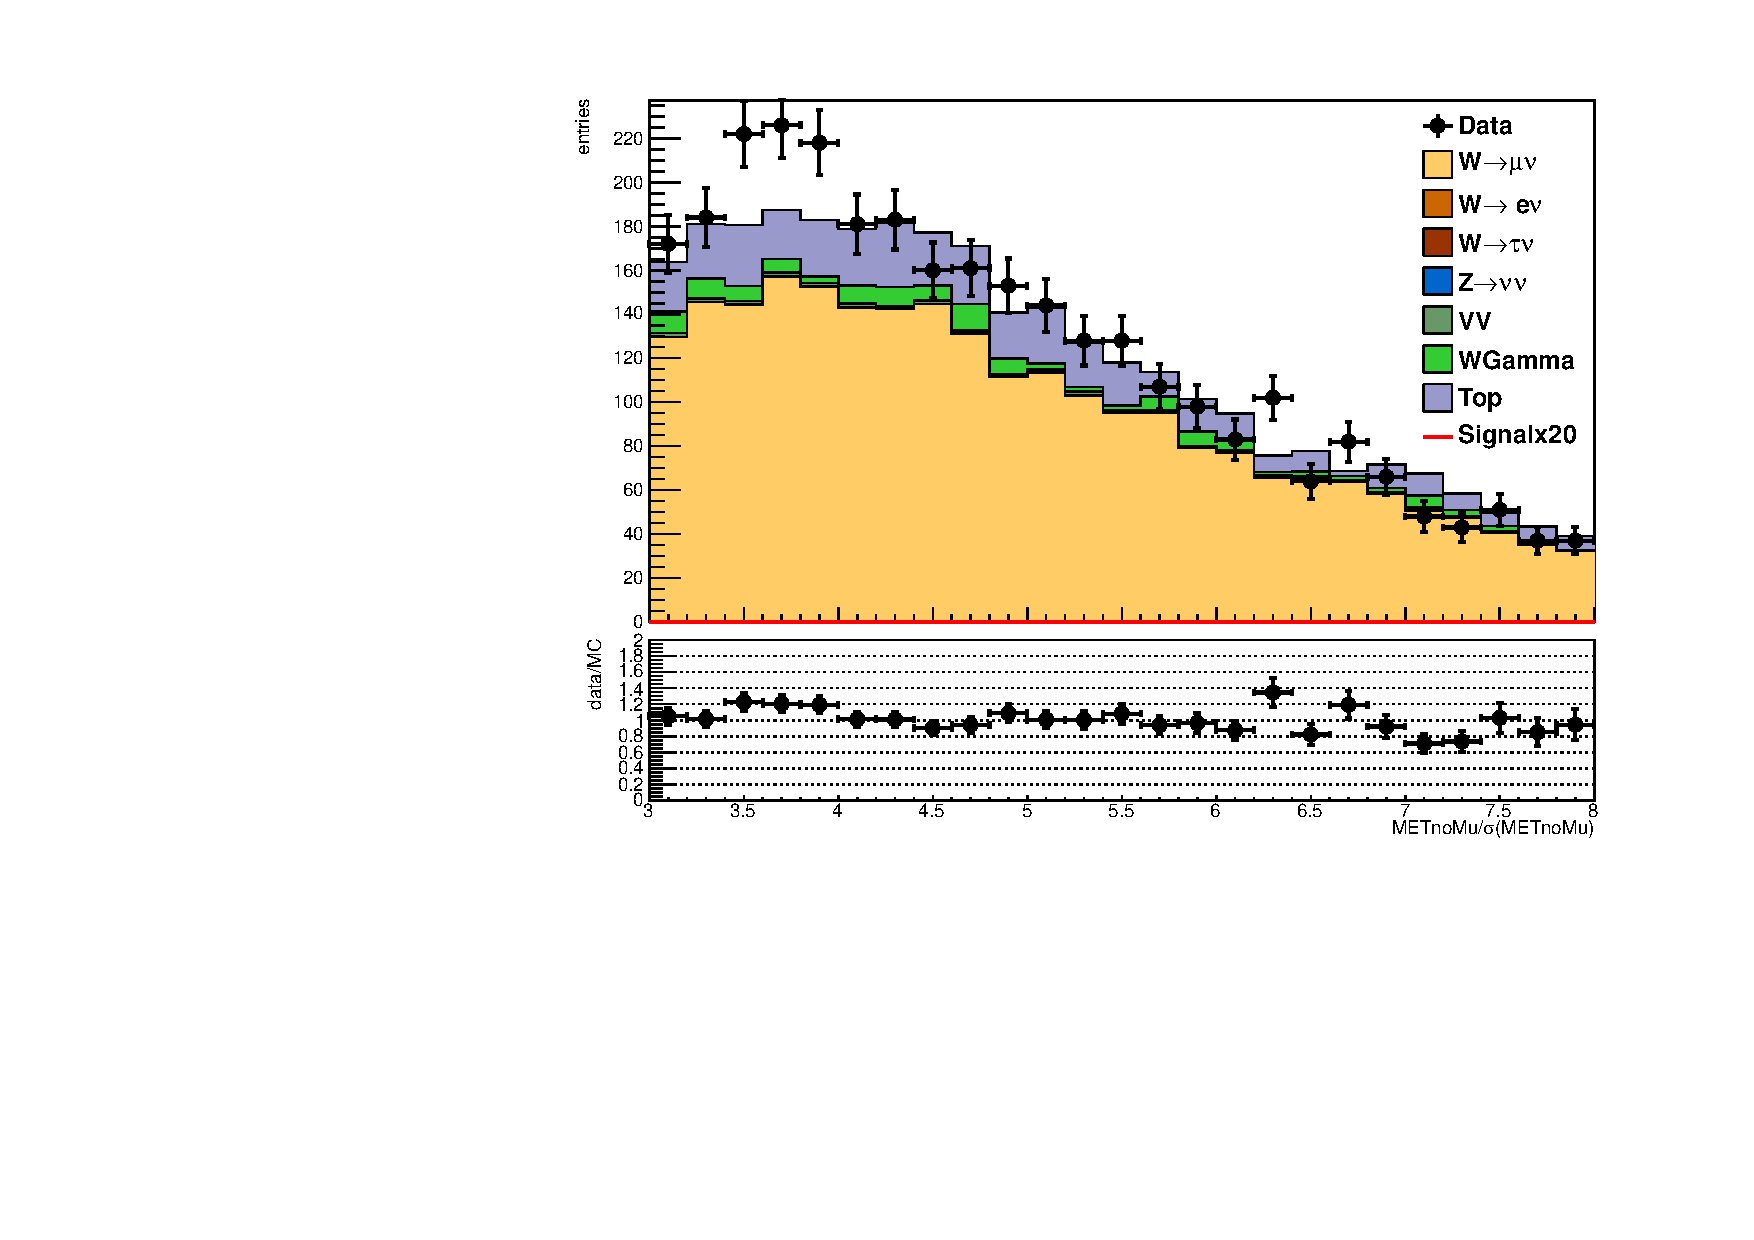
\includegraphics[width=\textwidth]{TalkPics/contplotsandpresel220914/output_contplots_rebinned2dweightsmumtcut/munu_metnomu_significance.pdf}
    \end{block}
  \end{columns}
\end{frame}

\begin{frame}
  \frametitle{Try mt cut}
  \begin{columns}
    \column{.5\textwidth}
    \begin{block}{\scriptsize mt - no mt cut}
      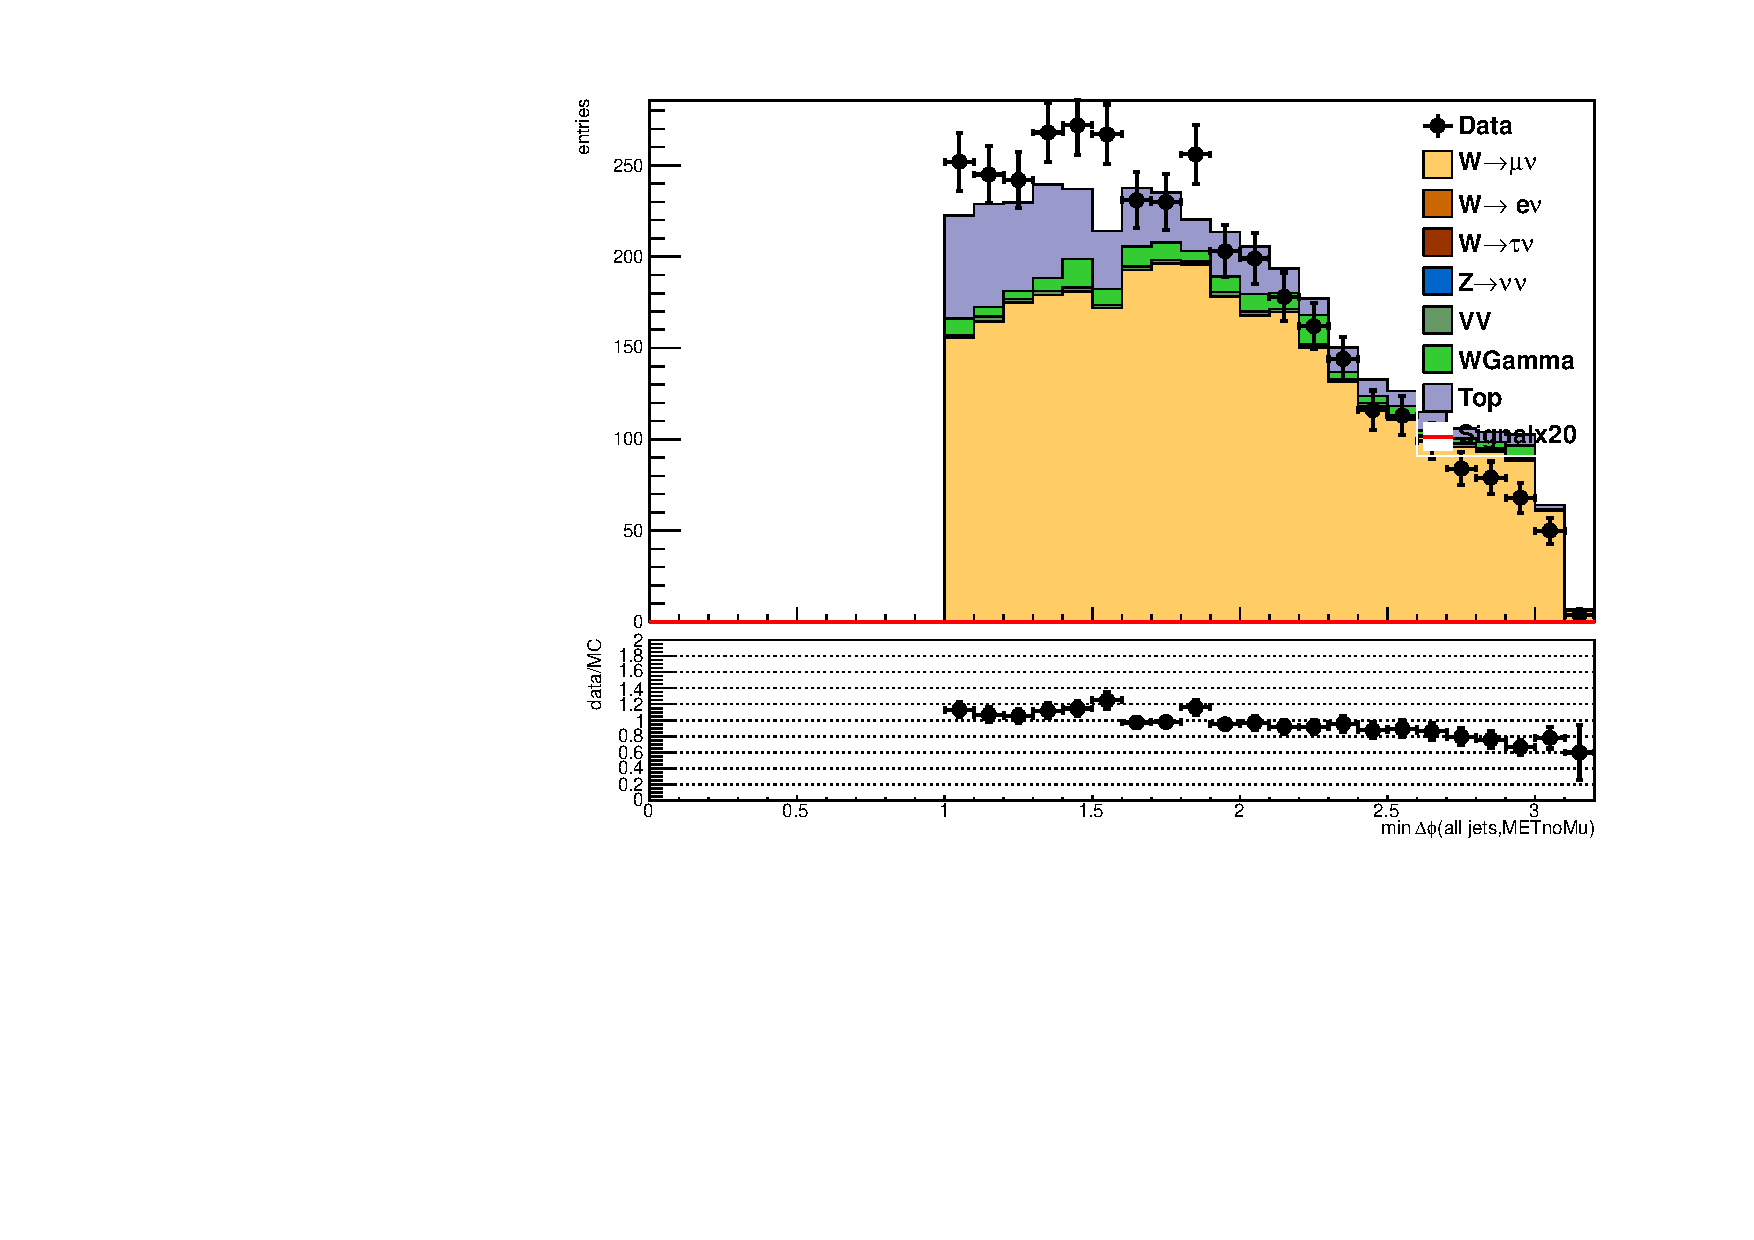
\includegraphics[width=\textwidth]{TalkPics/contplotsandpresel220914/output_contplots_rebinned2dweights/munu_alljetsmetnomu_mindphi.pdf}
    \end{block}
    \column{.5\textwidth}
    \begin{block}{\scriptsize mt - mt$>10$ GeV}
      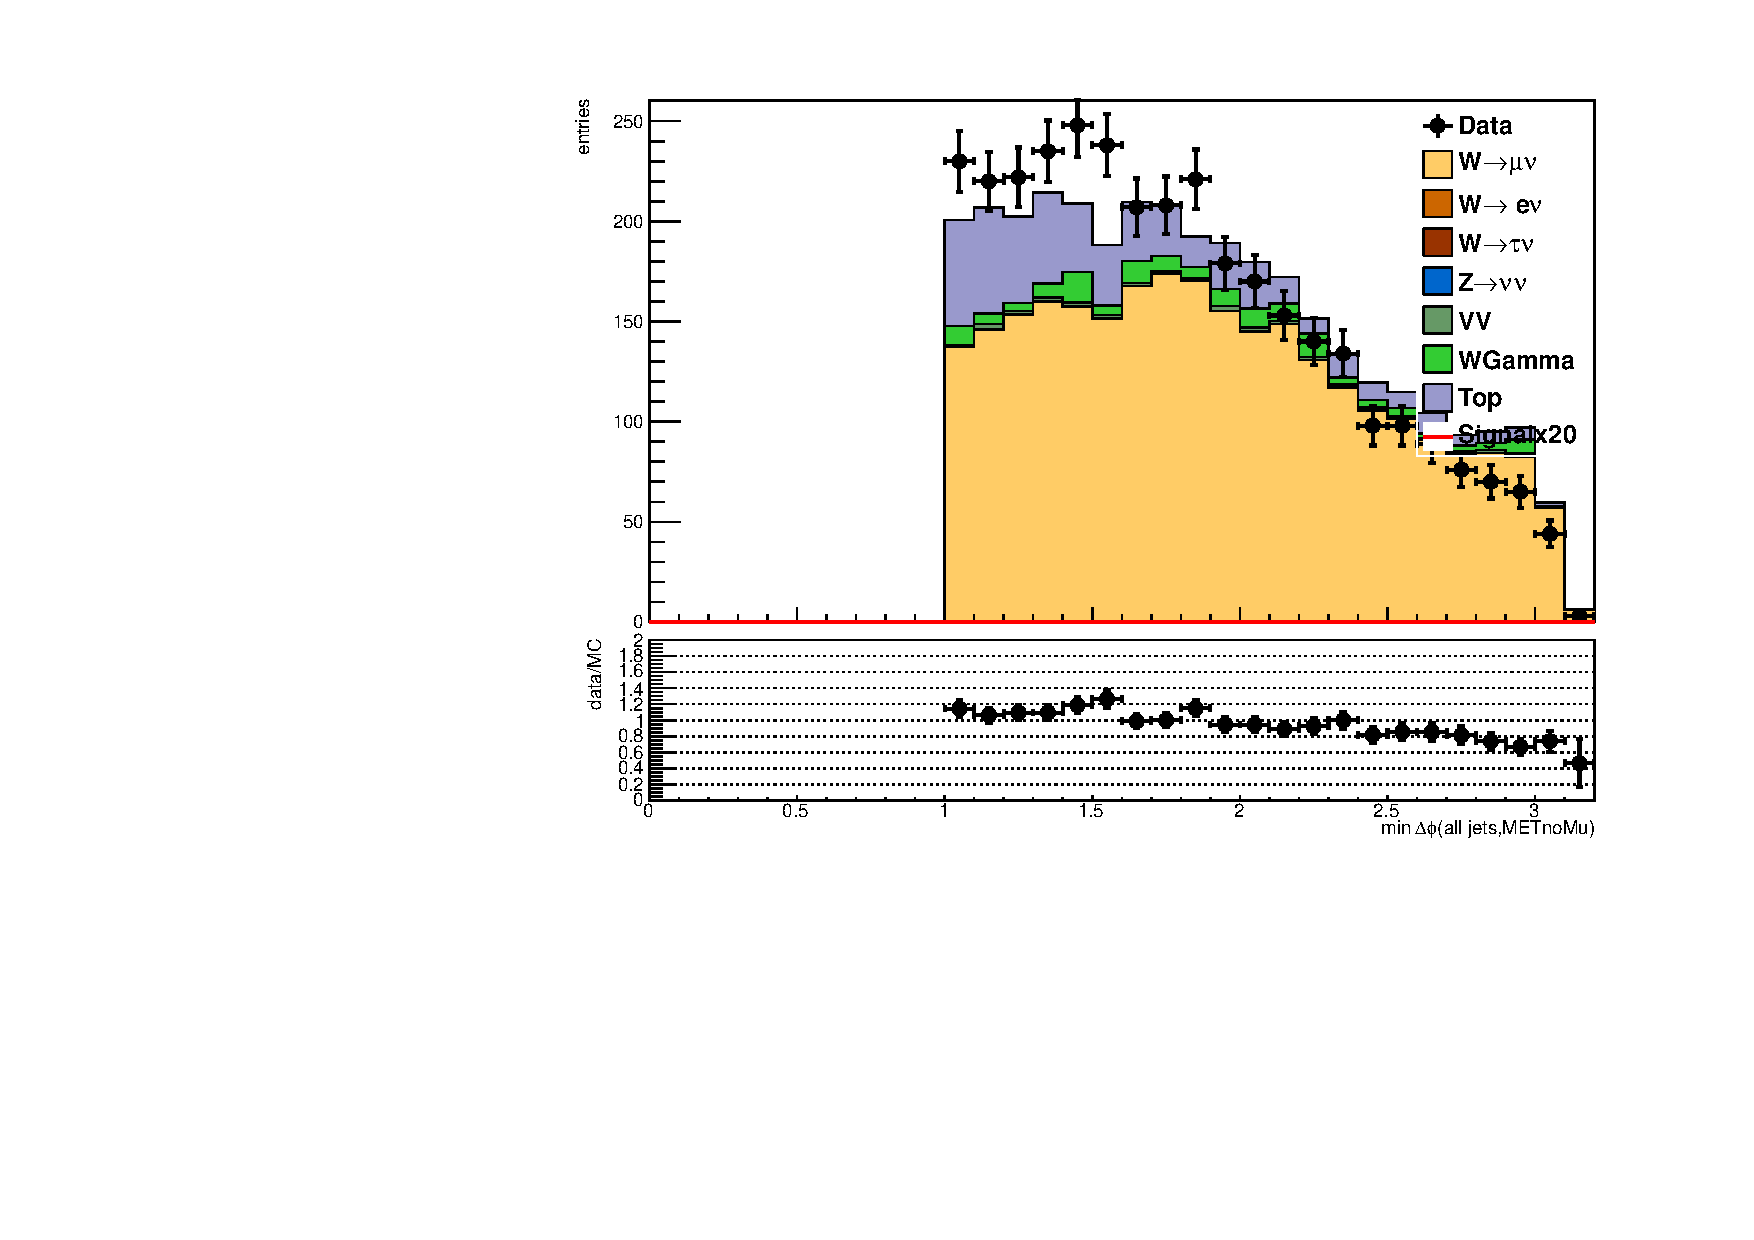
\includegraphics[width=\textwidth]{TalkPics/contplotsandpresel220914/output_contplots_rebinned2dweightsmumtcut/munu_alljetsmetnomu_mindphi.pdf}
    \end{block}
  \end{columns}
  \begin{block}{}
    \scriptsize
    \begin{itemize}
    \item Minor improvement in metnomu
    \item Doesn't improve other distributions
    \end{itemize}
  \end{block}
\end{frame}


\begin{frame}
  \frametitle{Conclusions}
  \label{lastframe}

  \begin{block}{}
    \scriptsize
    \begin{itemize}
    \item New trigger weights give minor improvement
    \item Mjj consistently off in first two bins
    \item Munu still has shape disagreements
    \item Looks like MC deficits are in areas of munu region where QCD would be expected
    \item[-] tried a transverse mass cut - no significant improvement
    \item[-] also tried tightening jetmet mindphi cut for munu region - no significant improvement
    \end{itemize}
  \end{block}

\end{frame}

\begin{frame}
  \frametitle{Backup}
\end{frame}


%NEW BINNED J2PT PLOTS
\begin{frame}
  \frametitle{New control plots - mumu}
  \begin{columns}
    \column{.5\textwidth}
    \begin{block}{Jet 1 pt}
      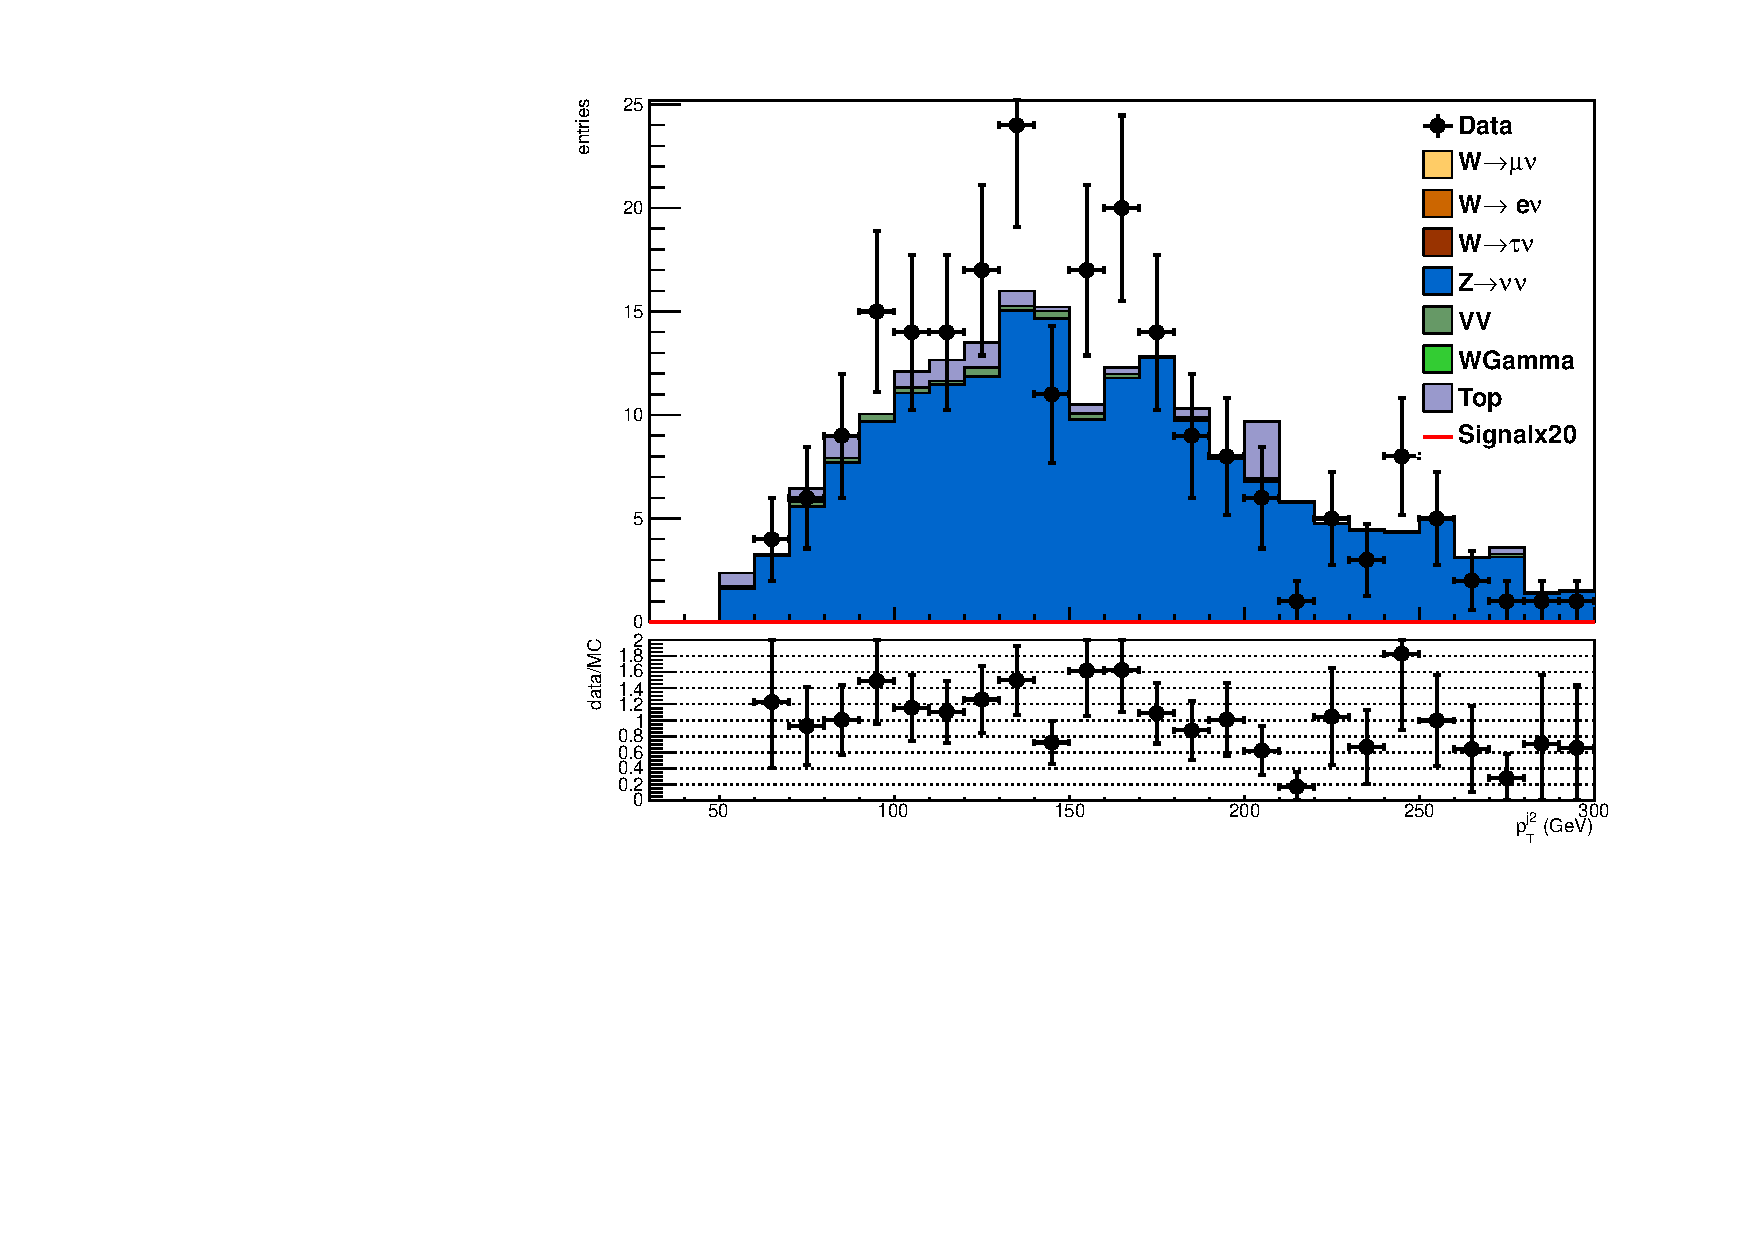
\includegraphics[width=\textwidth]{TalkPics/contplotsandpresel220914/output_contplots_rebinned2dweights/mumu_jet1_pt.pdf}
    \end{block}
    \column{.5\textwidth}
    \begin{block}{Jet 2 pt}
      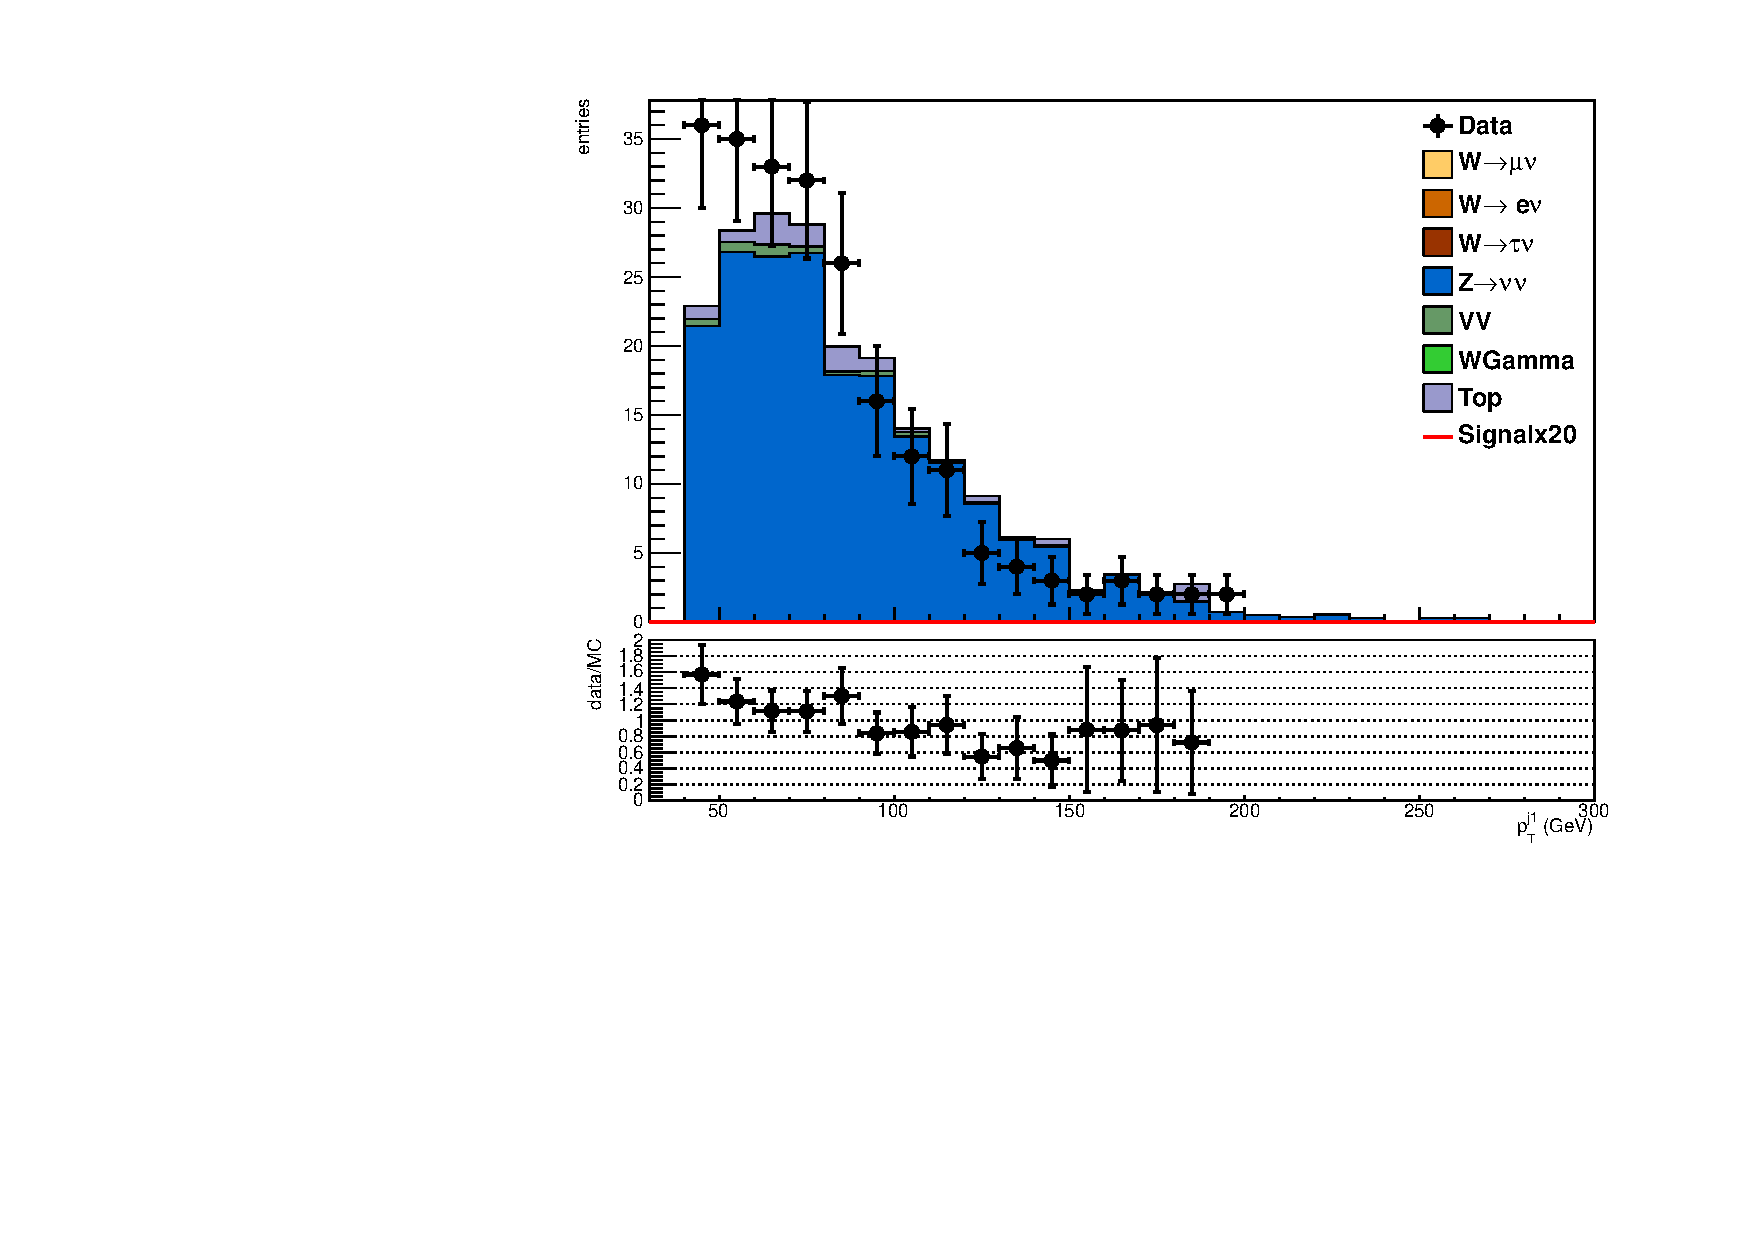
\includegraphics[width=\textwidth]{TalkPics/contplotsandpresel220914/output_contplots_rebinned2dweights/mumu_jet2_pt.pdf}
    \end{block}

  \end{columns}
\end{frame}

\begin{frame}
  \frametitle{New control plots - mumu}
  \begin{columns}
    \column{.5\textwidth}
    \begin{block}{METnomu}
      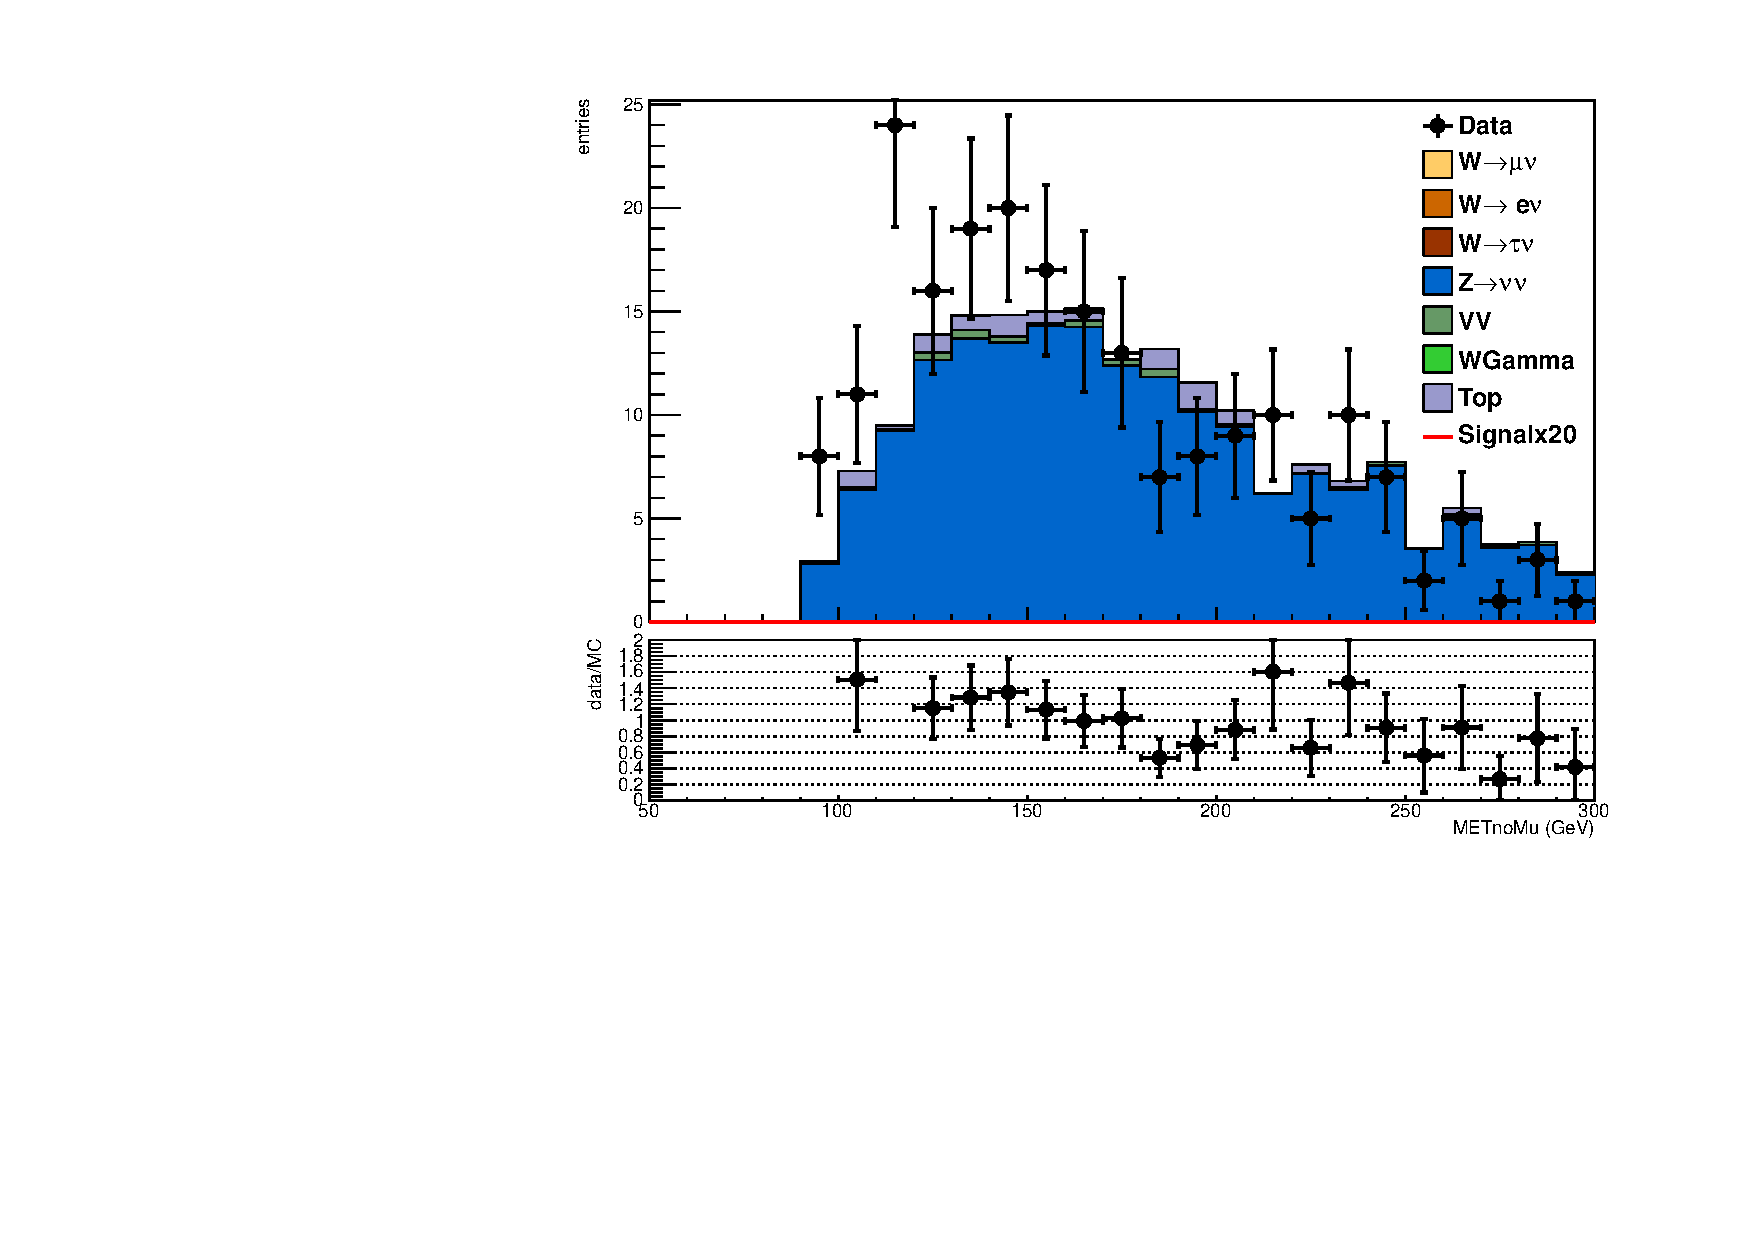
\includegraphics[width=\textwidth]{TalkPics/contplotsandpresel220914/output_contplots_rebinned2dweights/mumu_metnomuons.pdf}
    \end{block}
    \column{.5\textwidth}
    \begin{block}{METnomusig}
      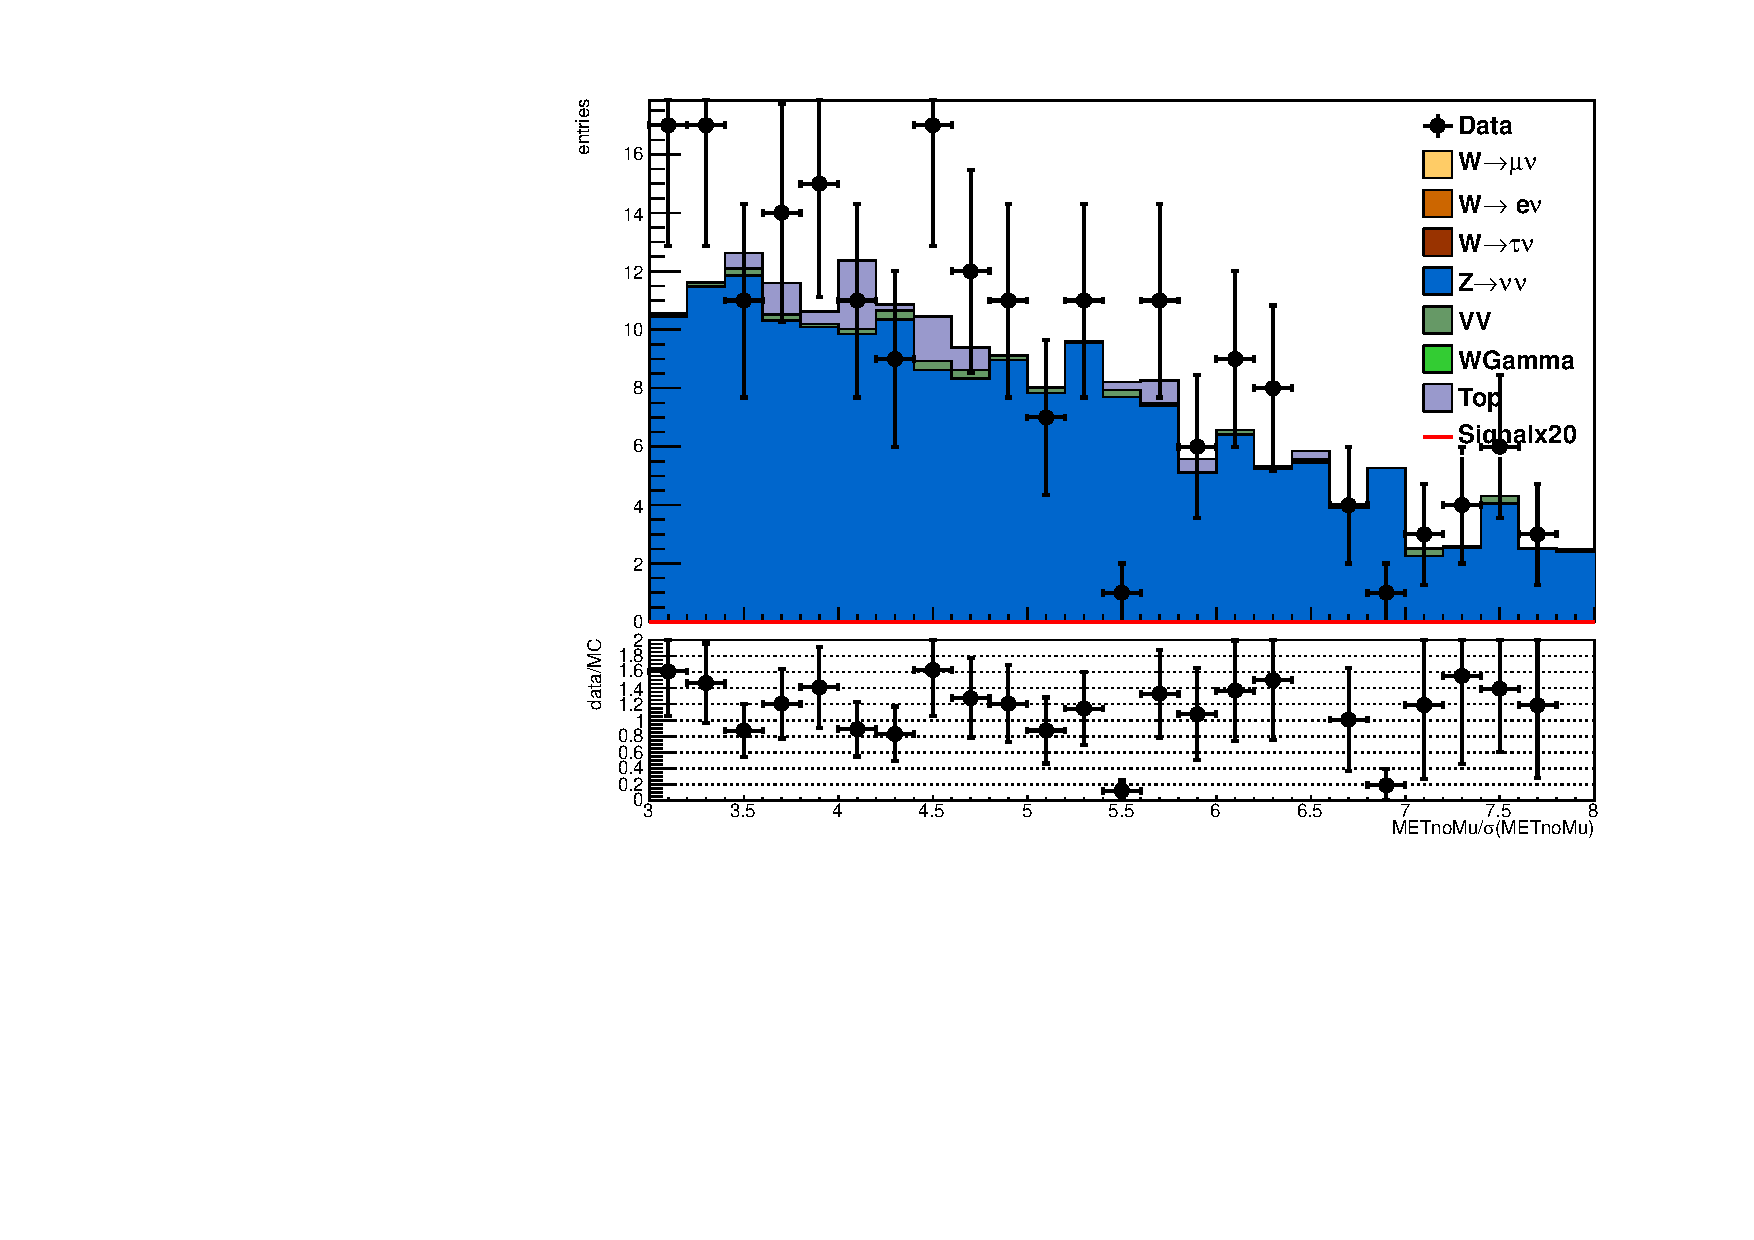
\includegraphics[width=\textwidth]{TalkPics/contplotsandpresel220914/output_contplots_rebinned2dweights/mumu_metnomu_significance.pdf}
    \end{block}

  \end{columns}
\end{frame}

\begin{frame}
  \frametitle{New control plots - mumu }
  \begin{columns}
    \column{.5\textwidth}
    \begin{block}{Mjj}
      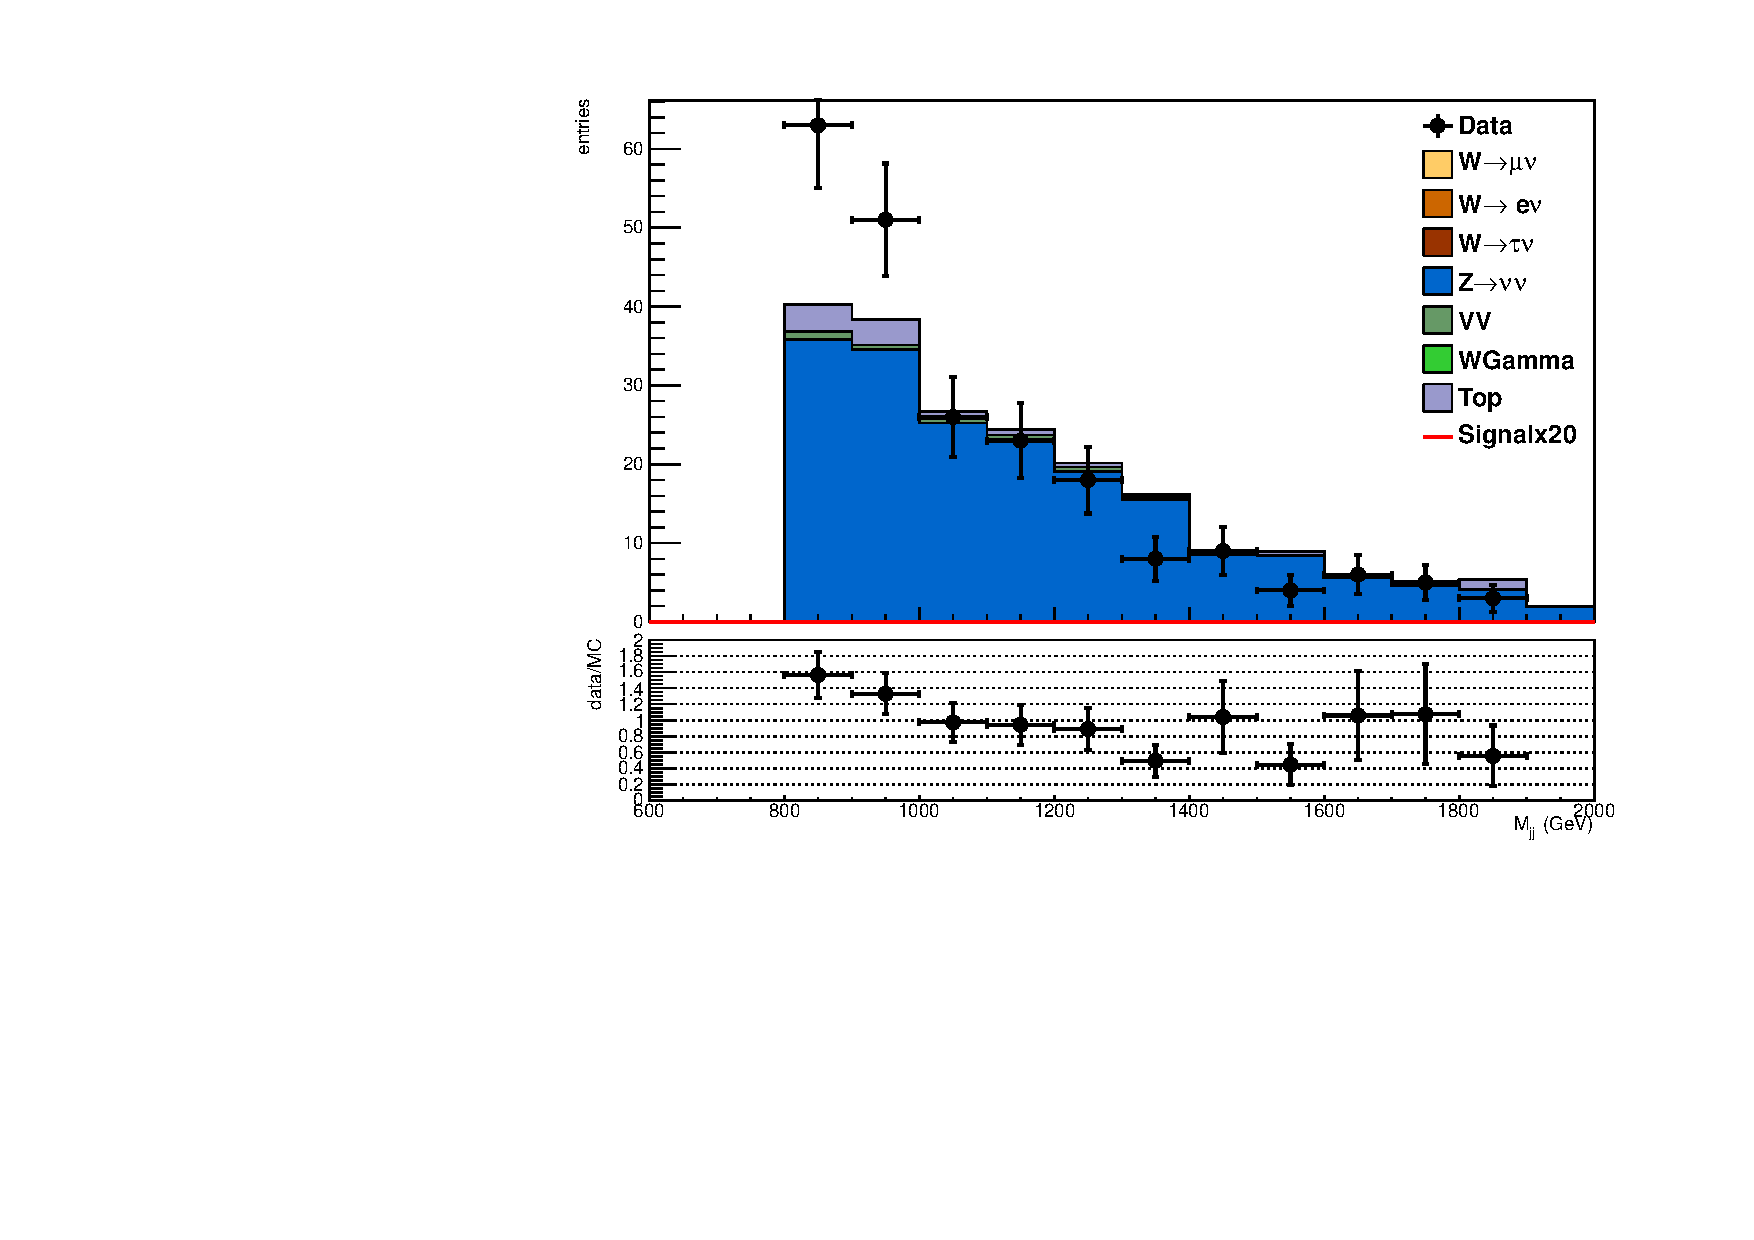
\includegraphics[width=\textwidth]{TalkPics/contplotsandpresel220914/output_contplots_rebinned2dweights/mumu_dijet_M.pdf}
    \end{block}
    \column{.5\textwidth}
    \begin{block}{dijet-metnomu pt fraction}
      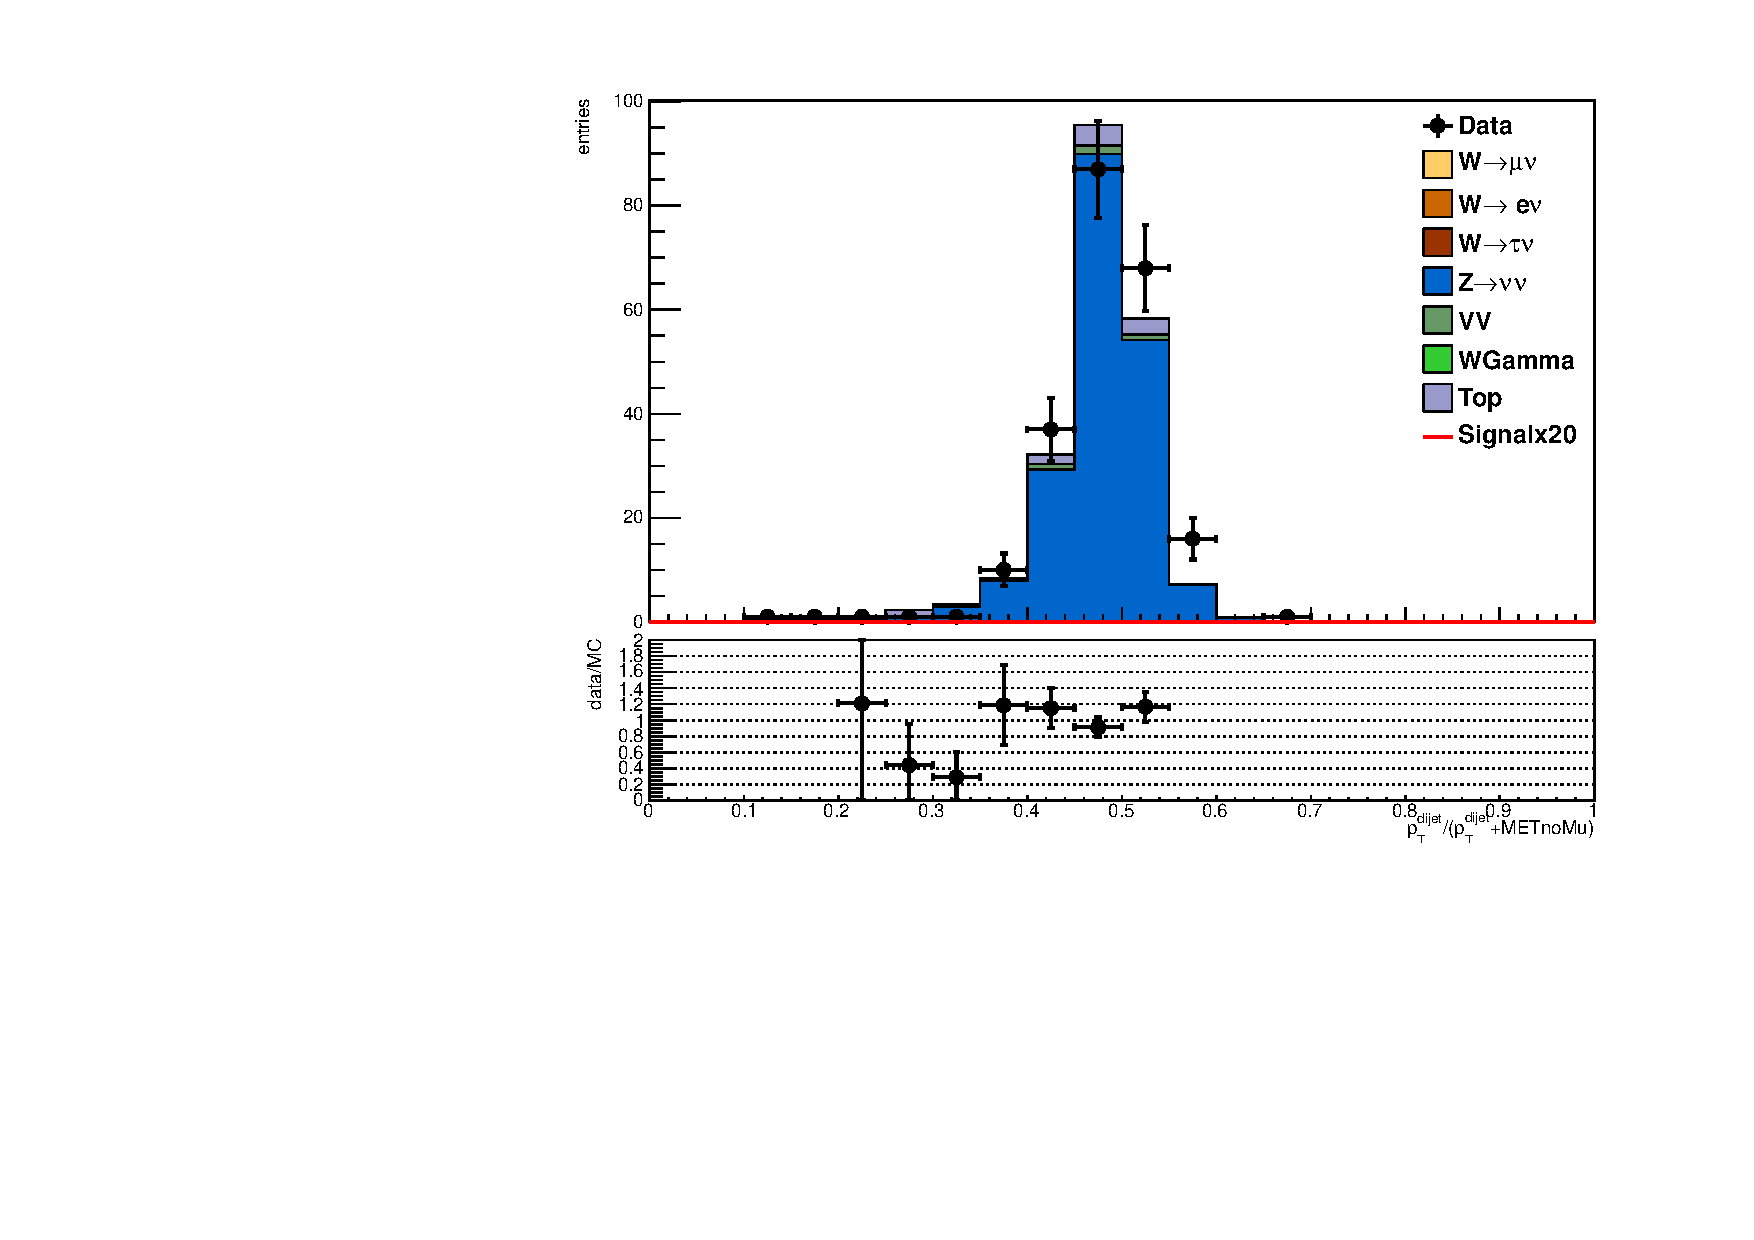
\includegraphics[width=\textwidth]{TalkPics/contplotsandpresel220914/output_contplots_rebinned2dweights/mumu_dijetmetnomu_ptfraction.pdf}
    \end{block}
  \end{columns}
\end{frame}

\begin{frame}
  \frametitle{New control plots -mumu}
  \begin{columns}
    \column{.5\textwidth}
    \begin{block}{Dphijj}
      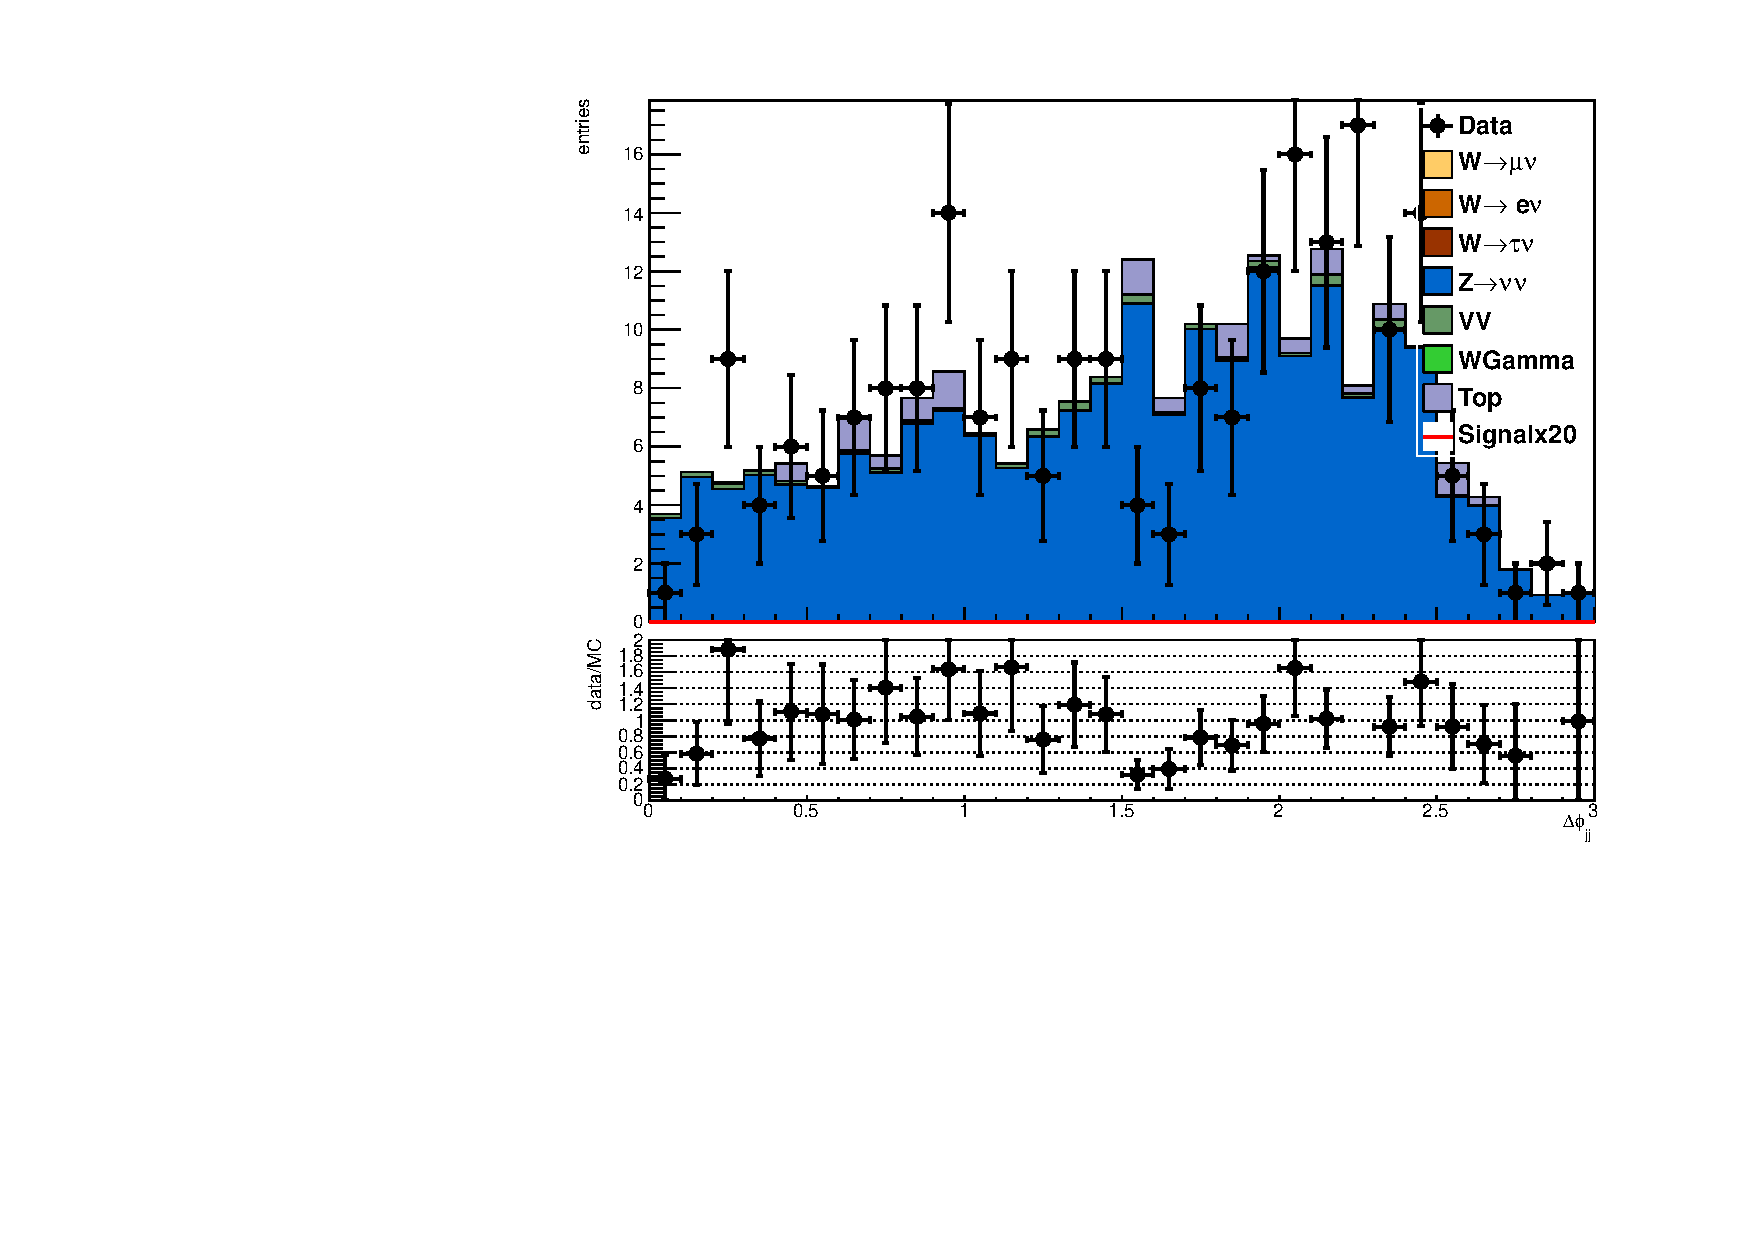
\includegraphics[width=\textwidth]{TalkPics/contplotsandpresel220914/output_contplots_rebinned2dweights/mumu_dijet_dphi.pdf}
    \end{block}
    \column{.5\textwidth}
    \begin{block}{Detajj}
      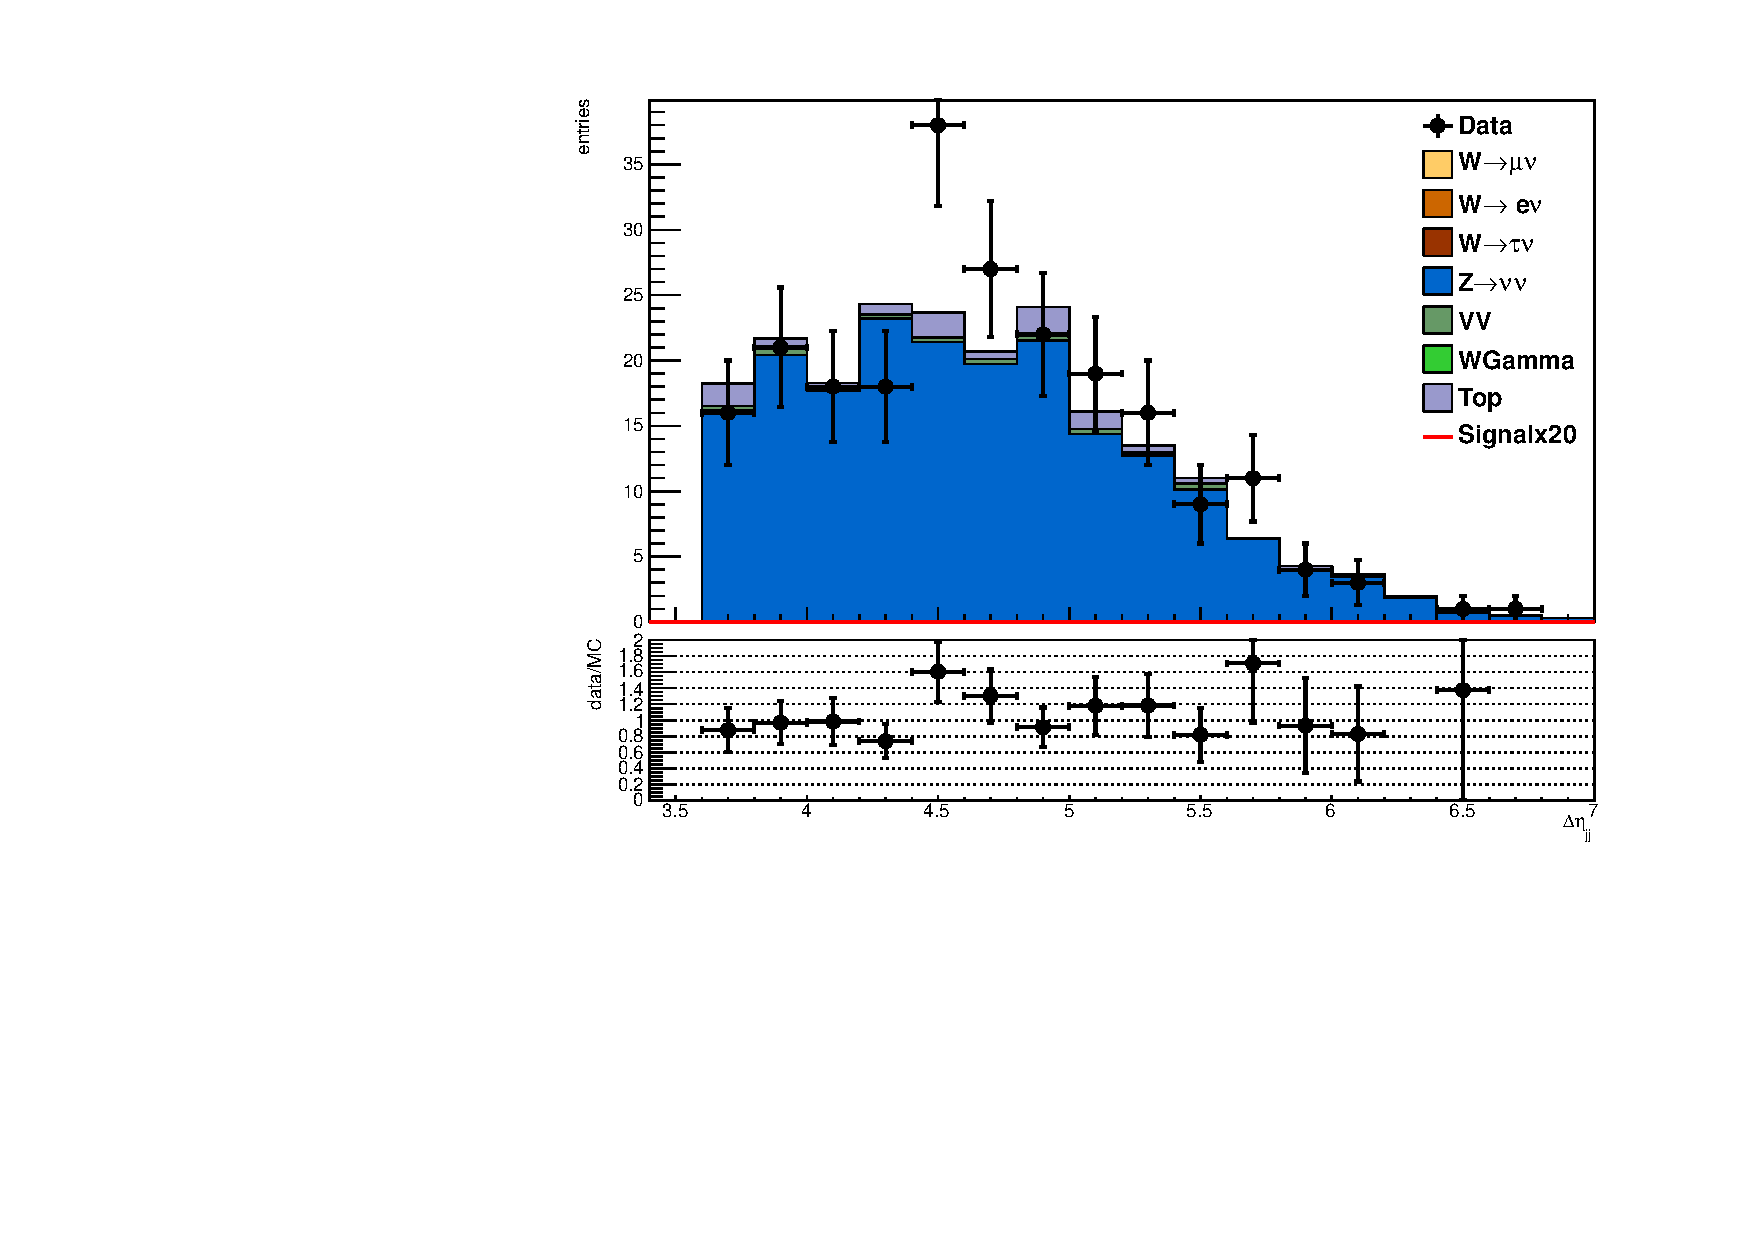
\includegraphics[width=\textwidth]{TalkPics/contplotsandpresel220914/output_contplots_rebinned2dweights/mumu_dijet_deta.pdf}
    \end{block}

  \end{columns}
\end{frame}

\begin{frame}
  \frametitle{New control plots -mumu}
  \begin{columns}
    \column{.5\textwidth}
    \begin{block}{Leading jets-met mindphi}
      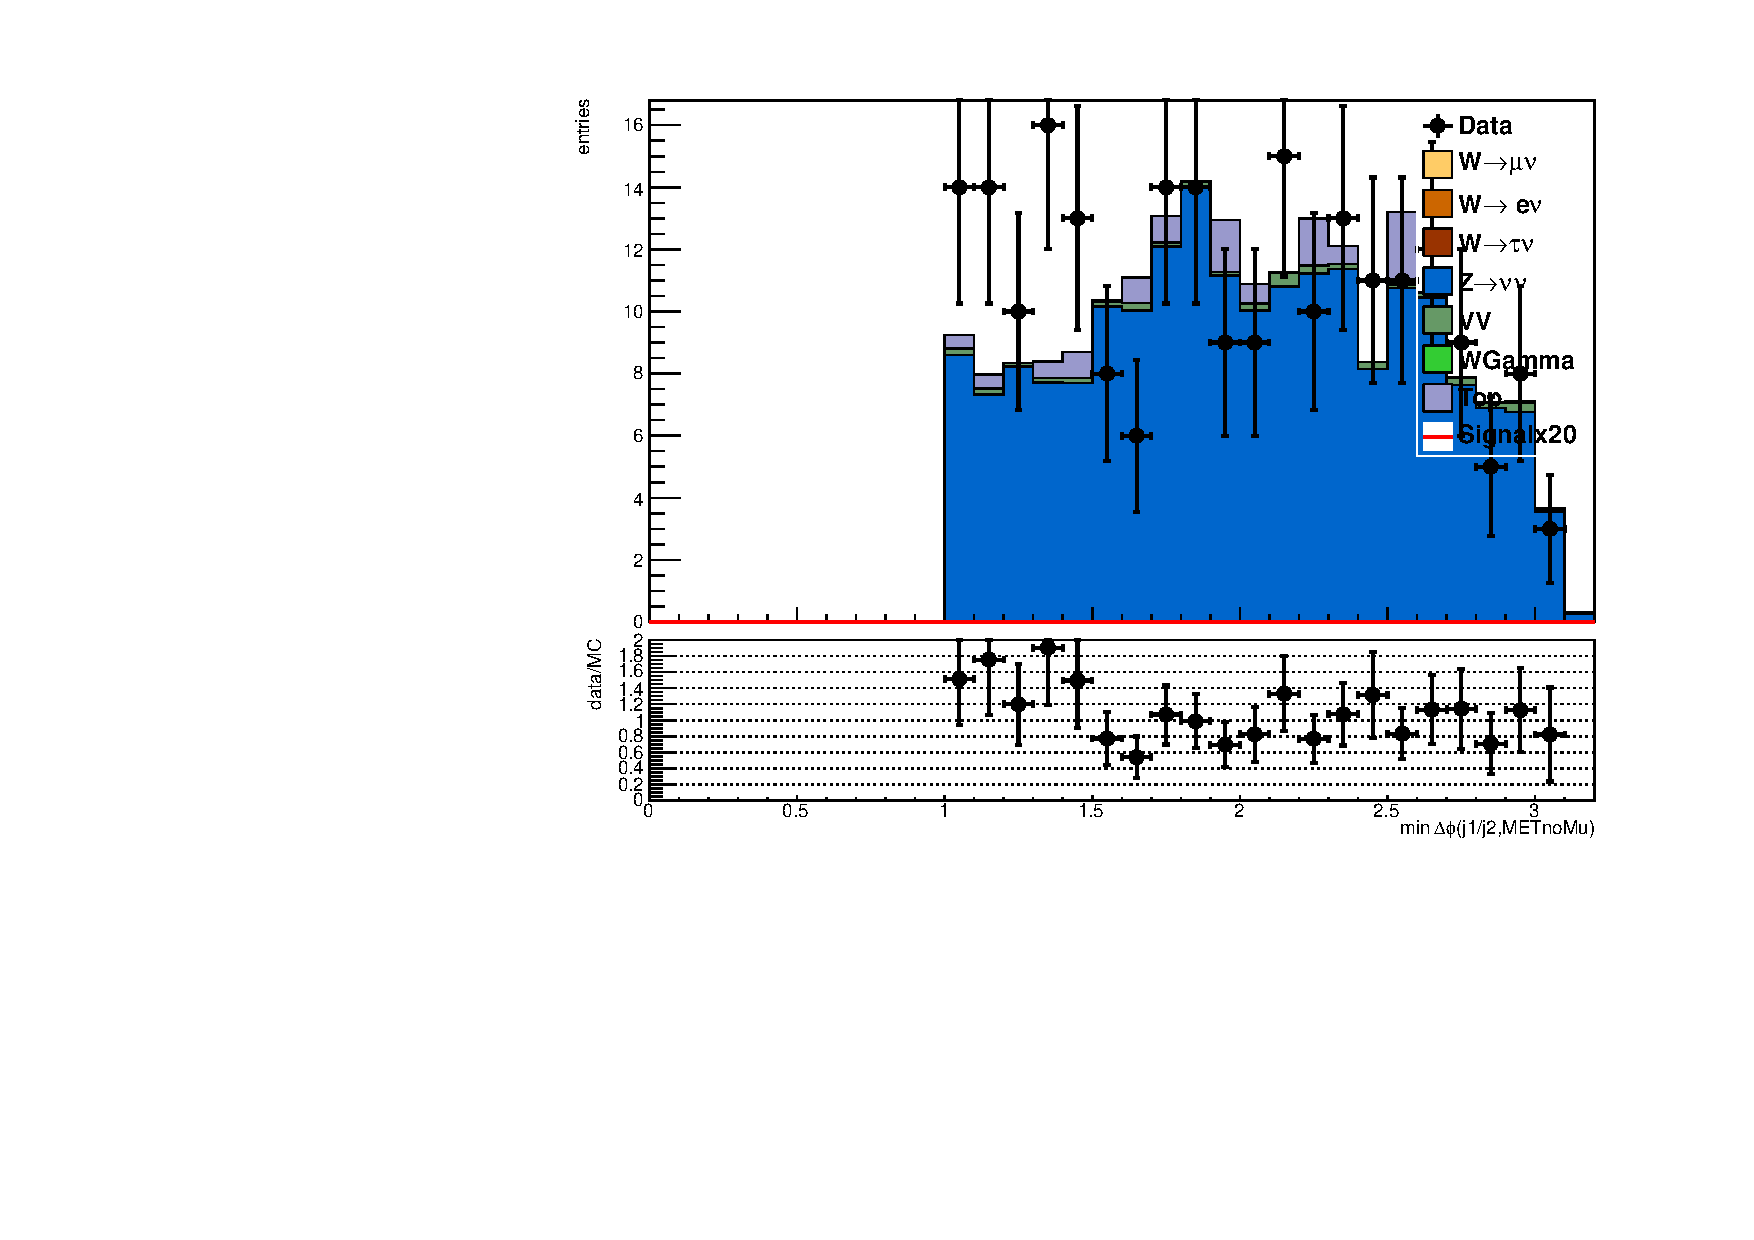
\includegraphics[width=\textwidth]{TalkPics/contplotsandpresel220914/output_contplots_rebinned2dweights/mumu_jetmetnomu_mindphi.pdf}
    \end{block}
    \column{.5\textwidth}
    \begin{block}{All jet-met mindphi}
      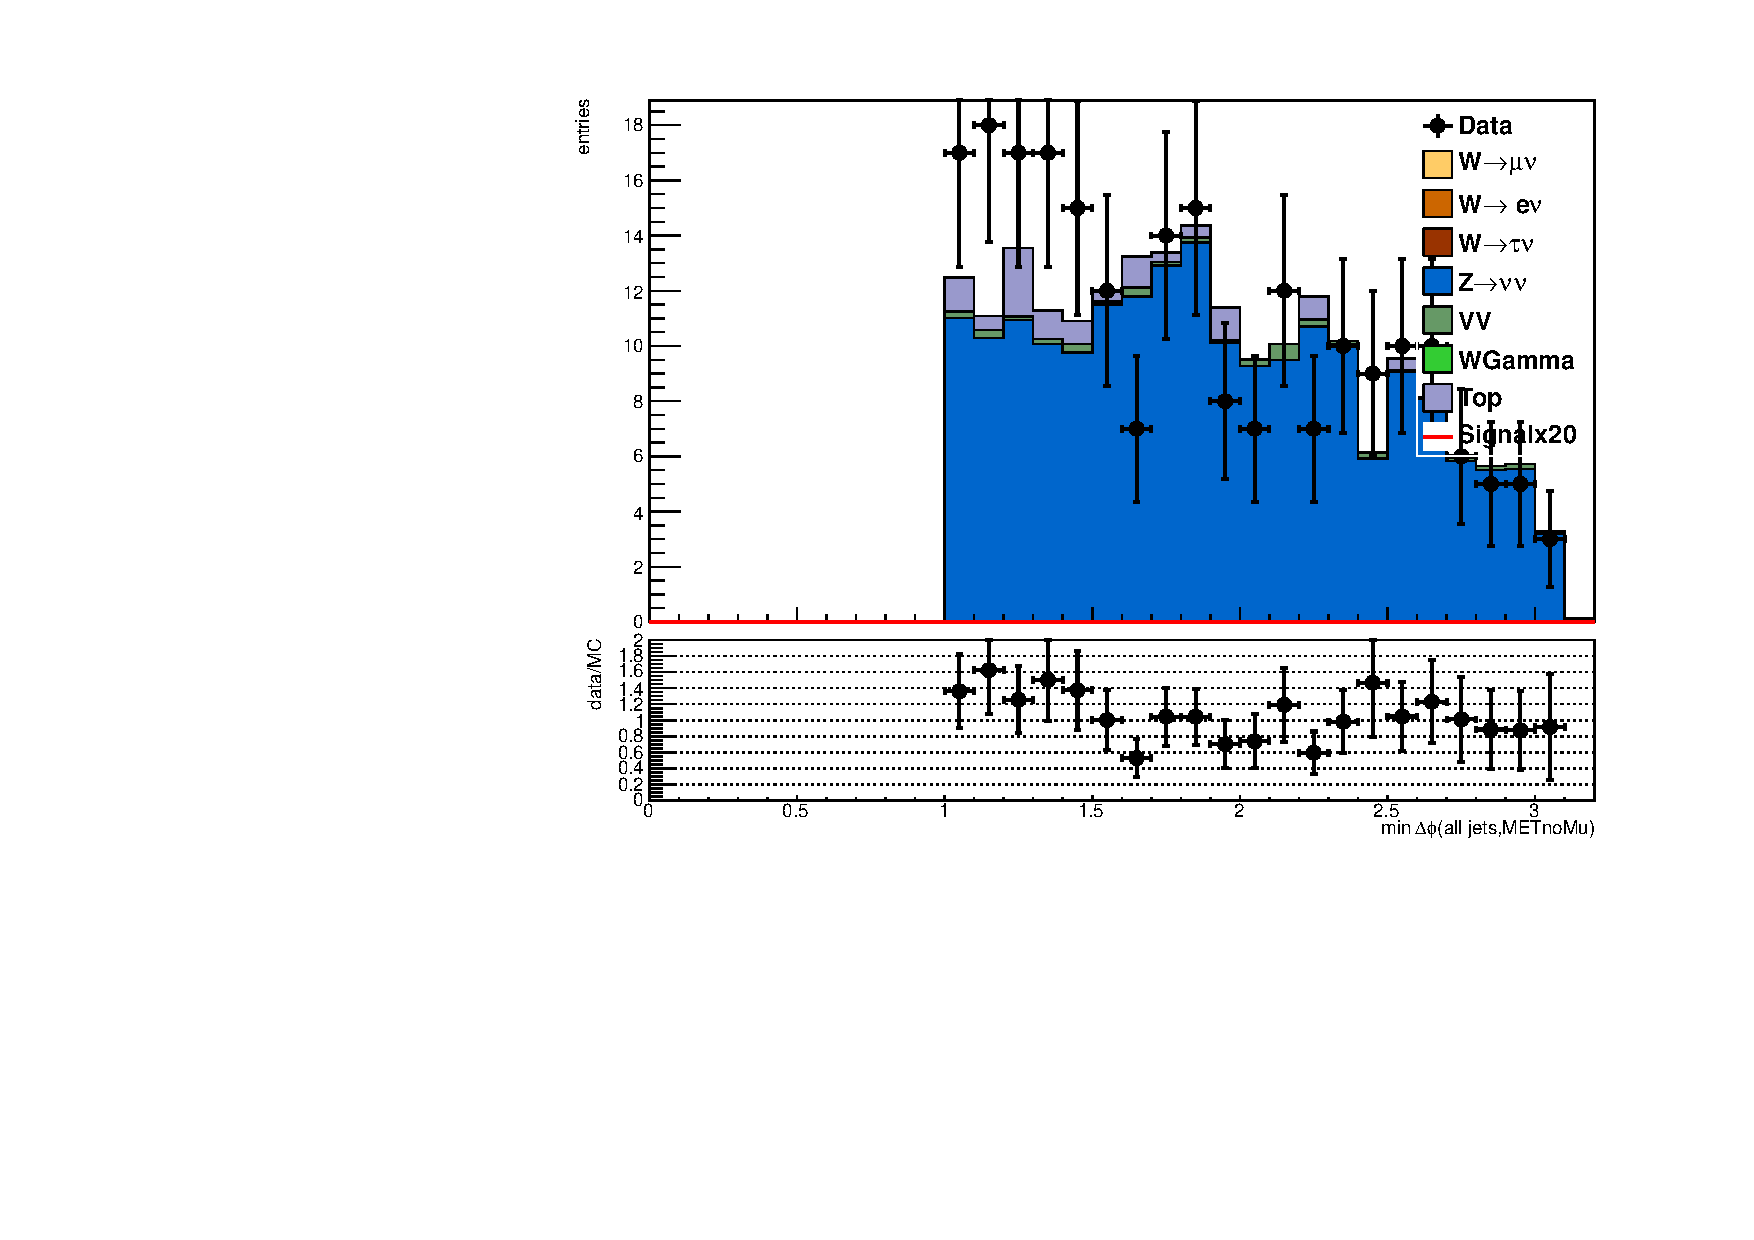
\includegraphics[width=\textwidth]{TalkPics/contplotsandpresel220914/output_contplots_rebinned2dweights/mumu_alljetsmetnomu_mindphi.pdf}
    \end{block}

  \end{columns}
\end{frame}

\begin{frame}
  \frametitle{New control plots -enu}
  \begin{columns}
    \column{.5\textwidth}
    \begin{block}{Jet 1 pt}
      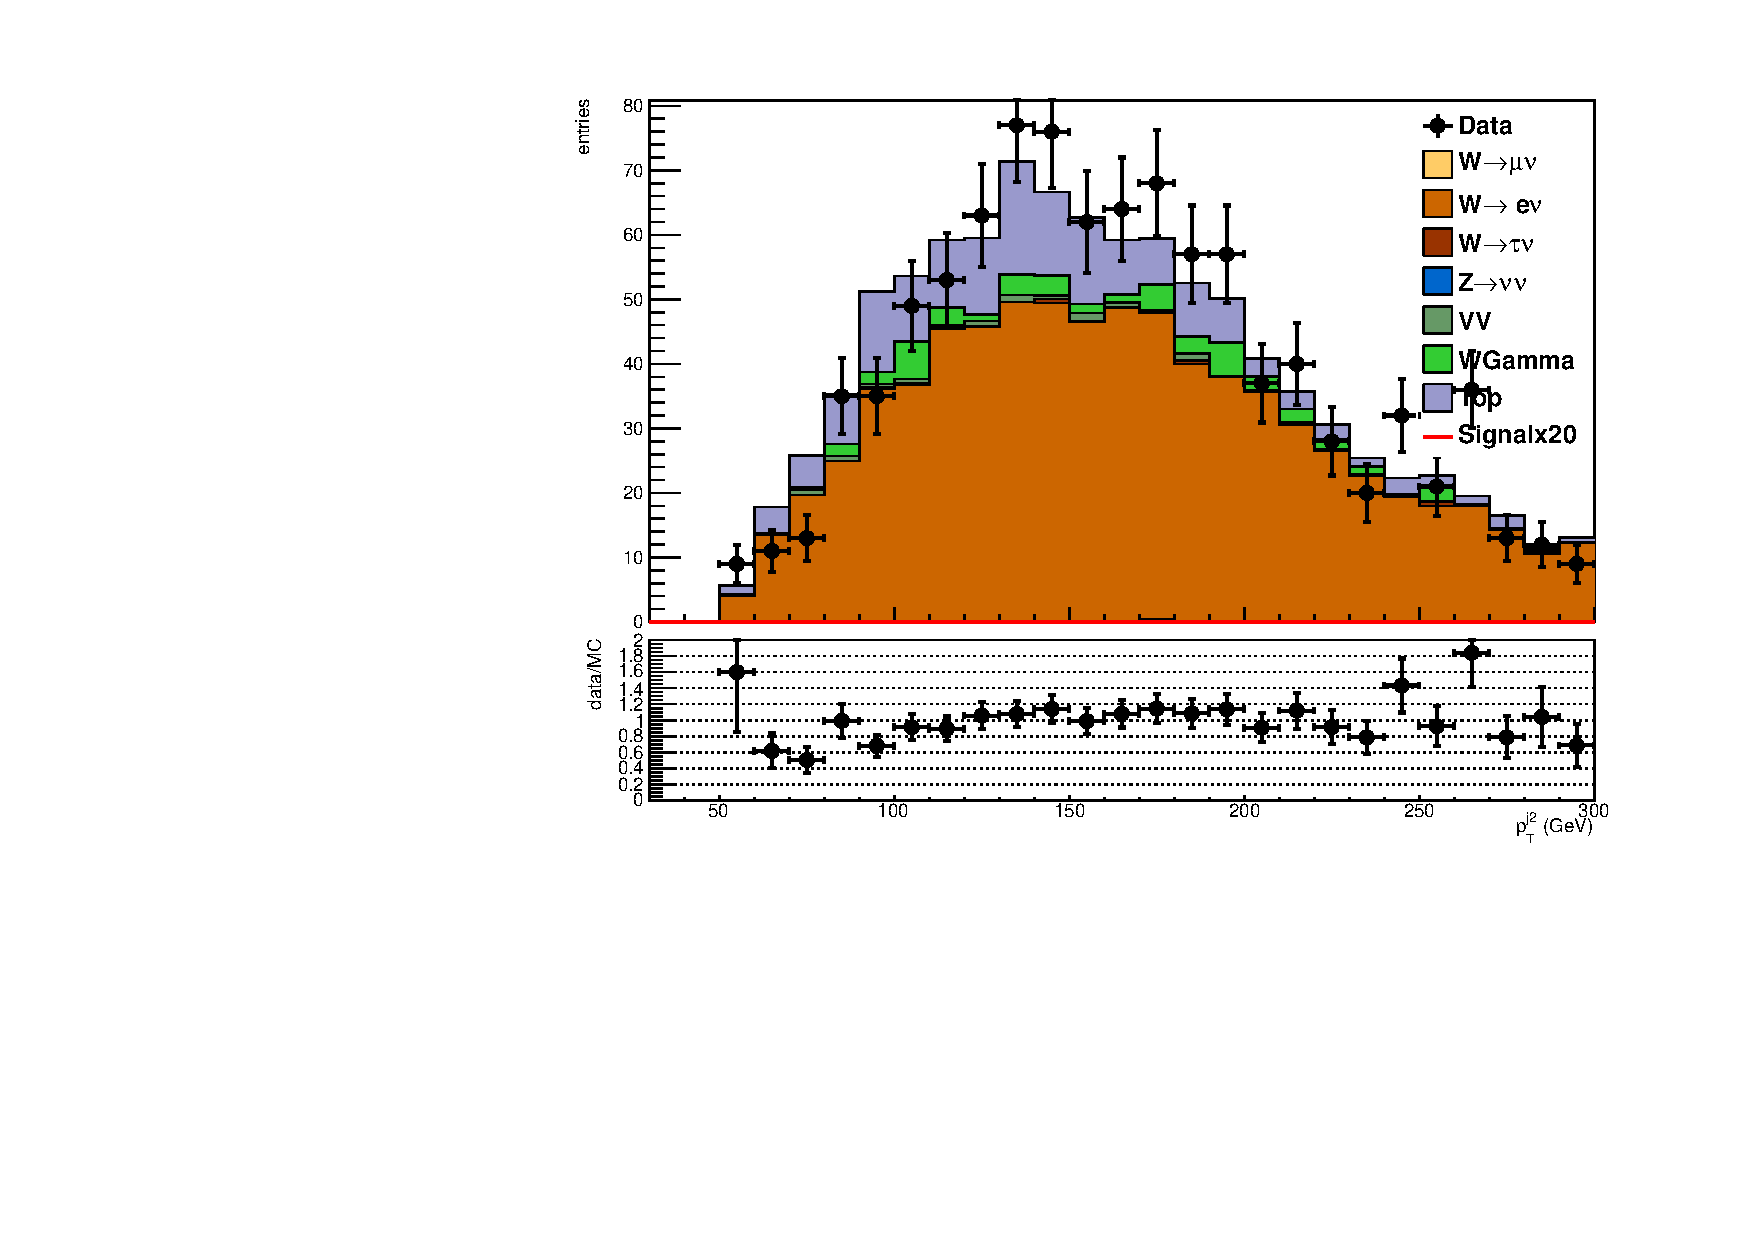
\includegraphics[width=\textwidth]{TalkPics/contplotsandpresel220914/output_contplots_rebinned2dweights/enu_jet1_pt.pdf}
    \end{block}
    \column{.5\textwidth}
    \begin{block}{Jet 2 pt}
      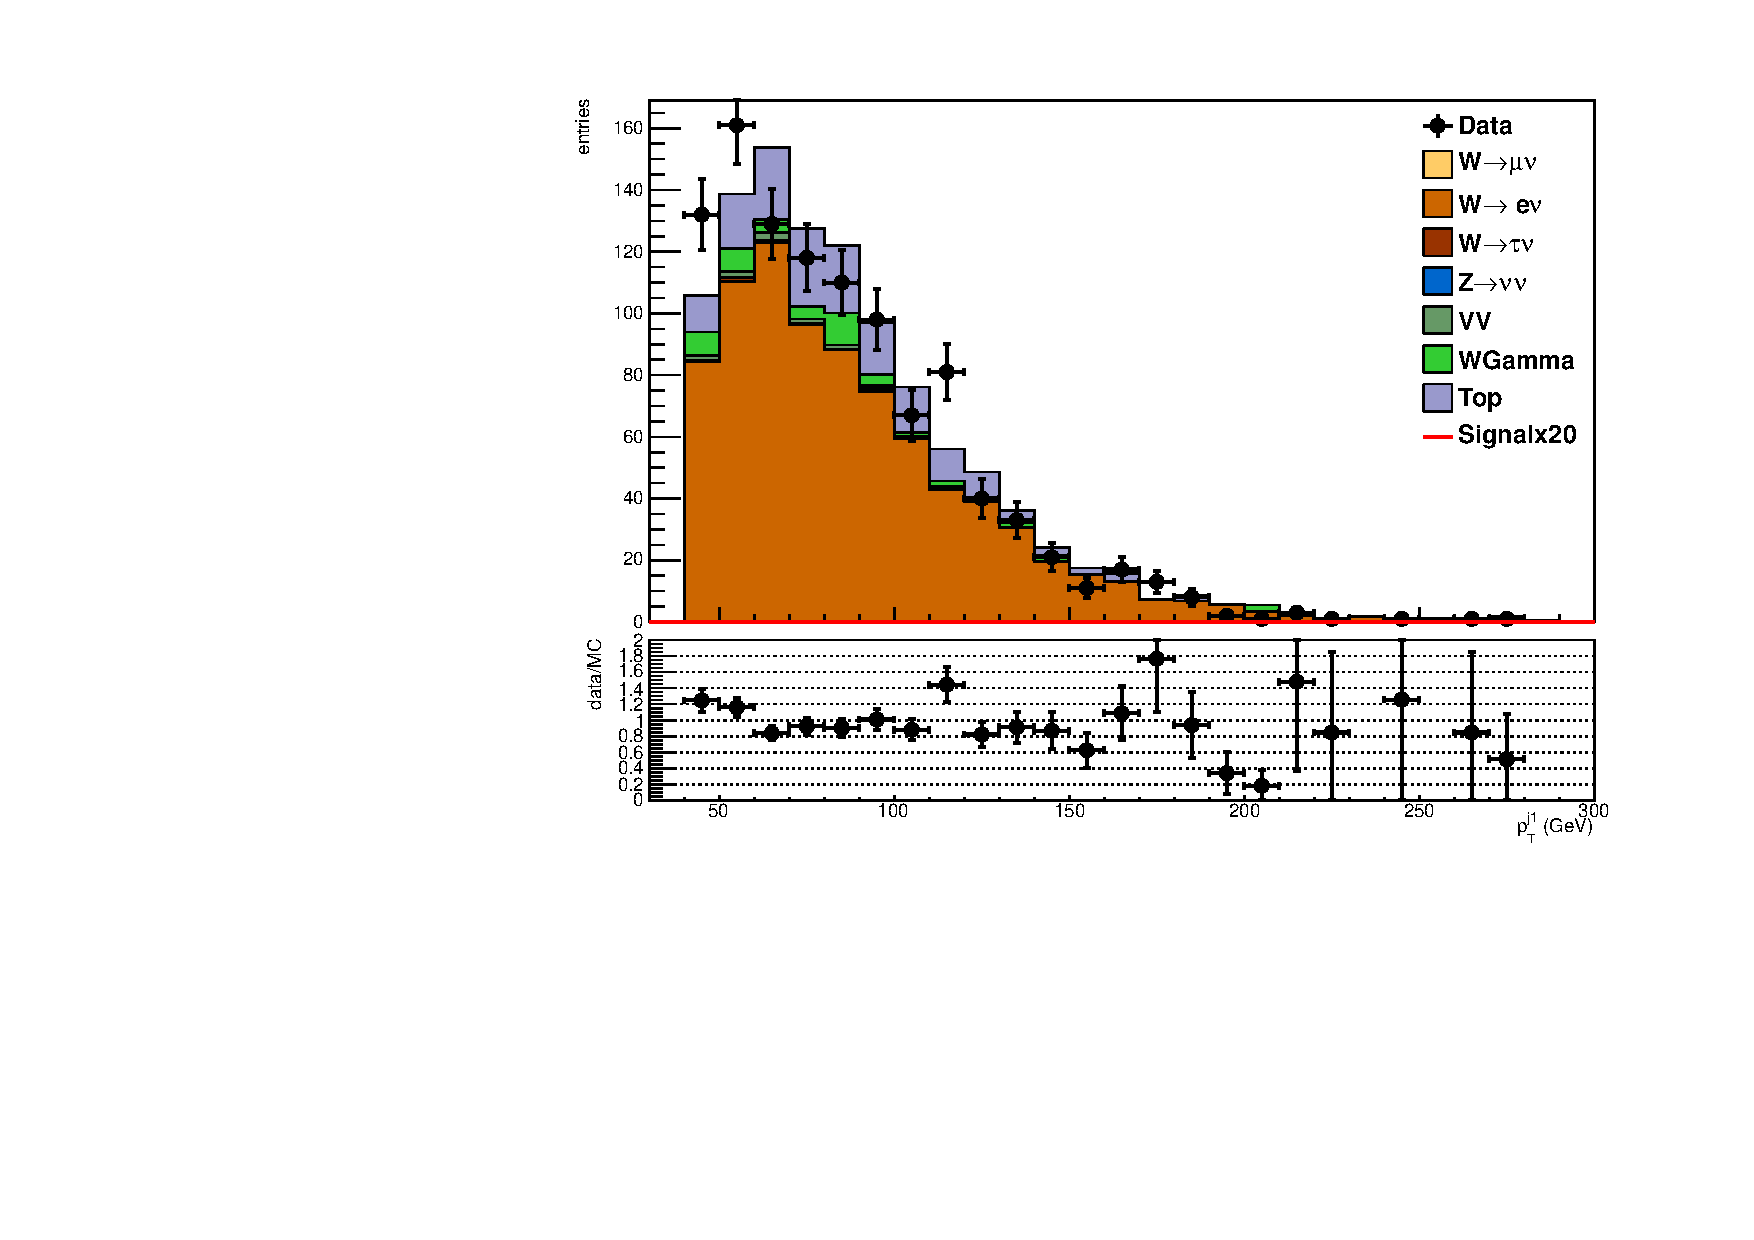
\includegraphics[width=\textwidth]{TalkPics/contplotsandpresel220914/output_contplots_rebinned2dweights/enu_jet2_pt.pdf}
    \end{block}

  \end{columns}
\end{frame}

\begin{frame}
  \frametitle{New control plots -enu}
  \begin{columns}
    \column{.5\textwidth}
    \begin{block}{METnomu}
      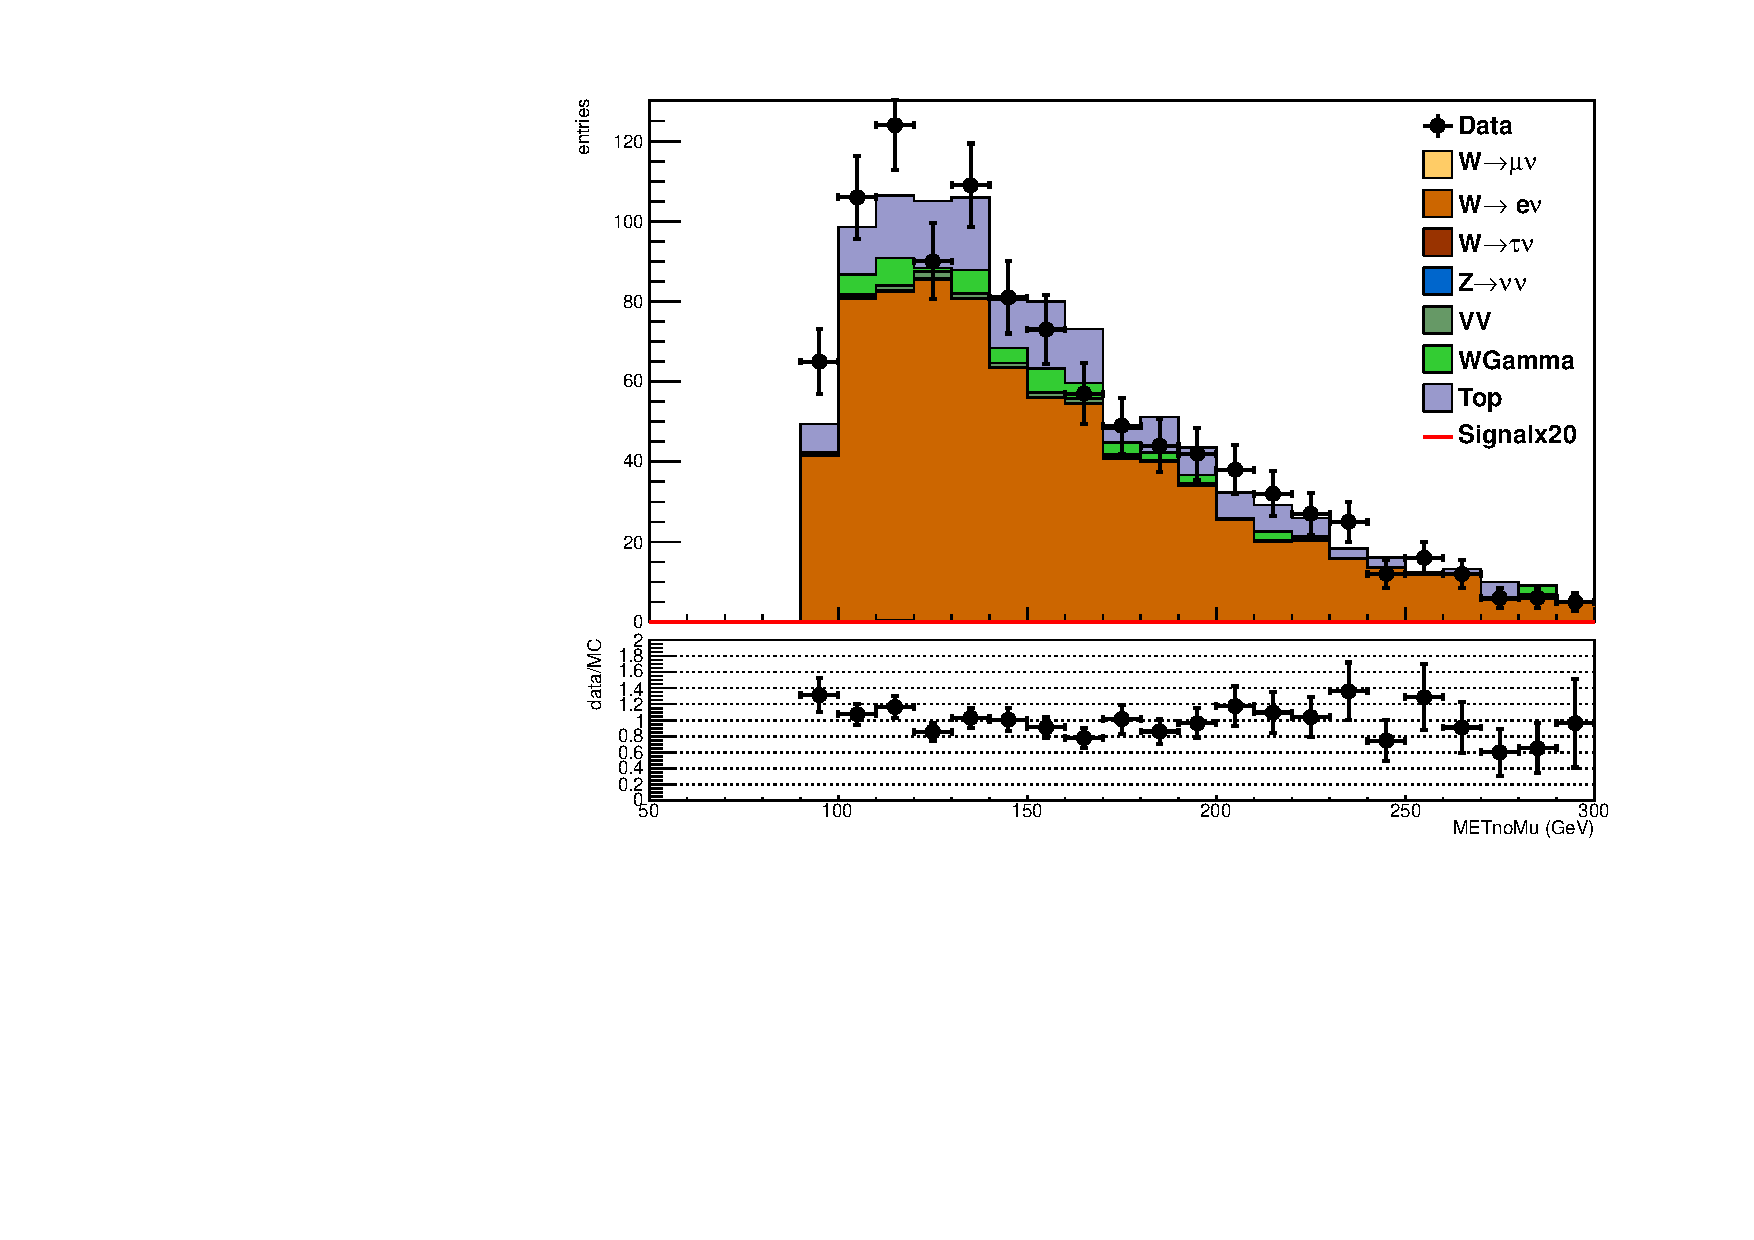
\includegraphics[width=\textwidth]{TalkPics/contplotsandpresel220914/output_contplots_rebinned2dweights/enu_metnomuons.pdf}
    \end{block}
    \column{.5\textwidth}
    \begin{block}{METnomusig}
      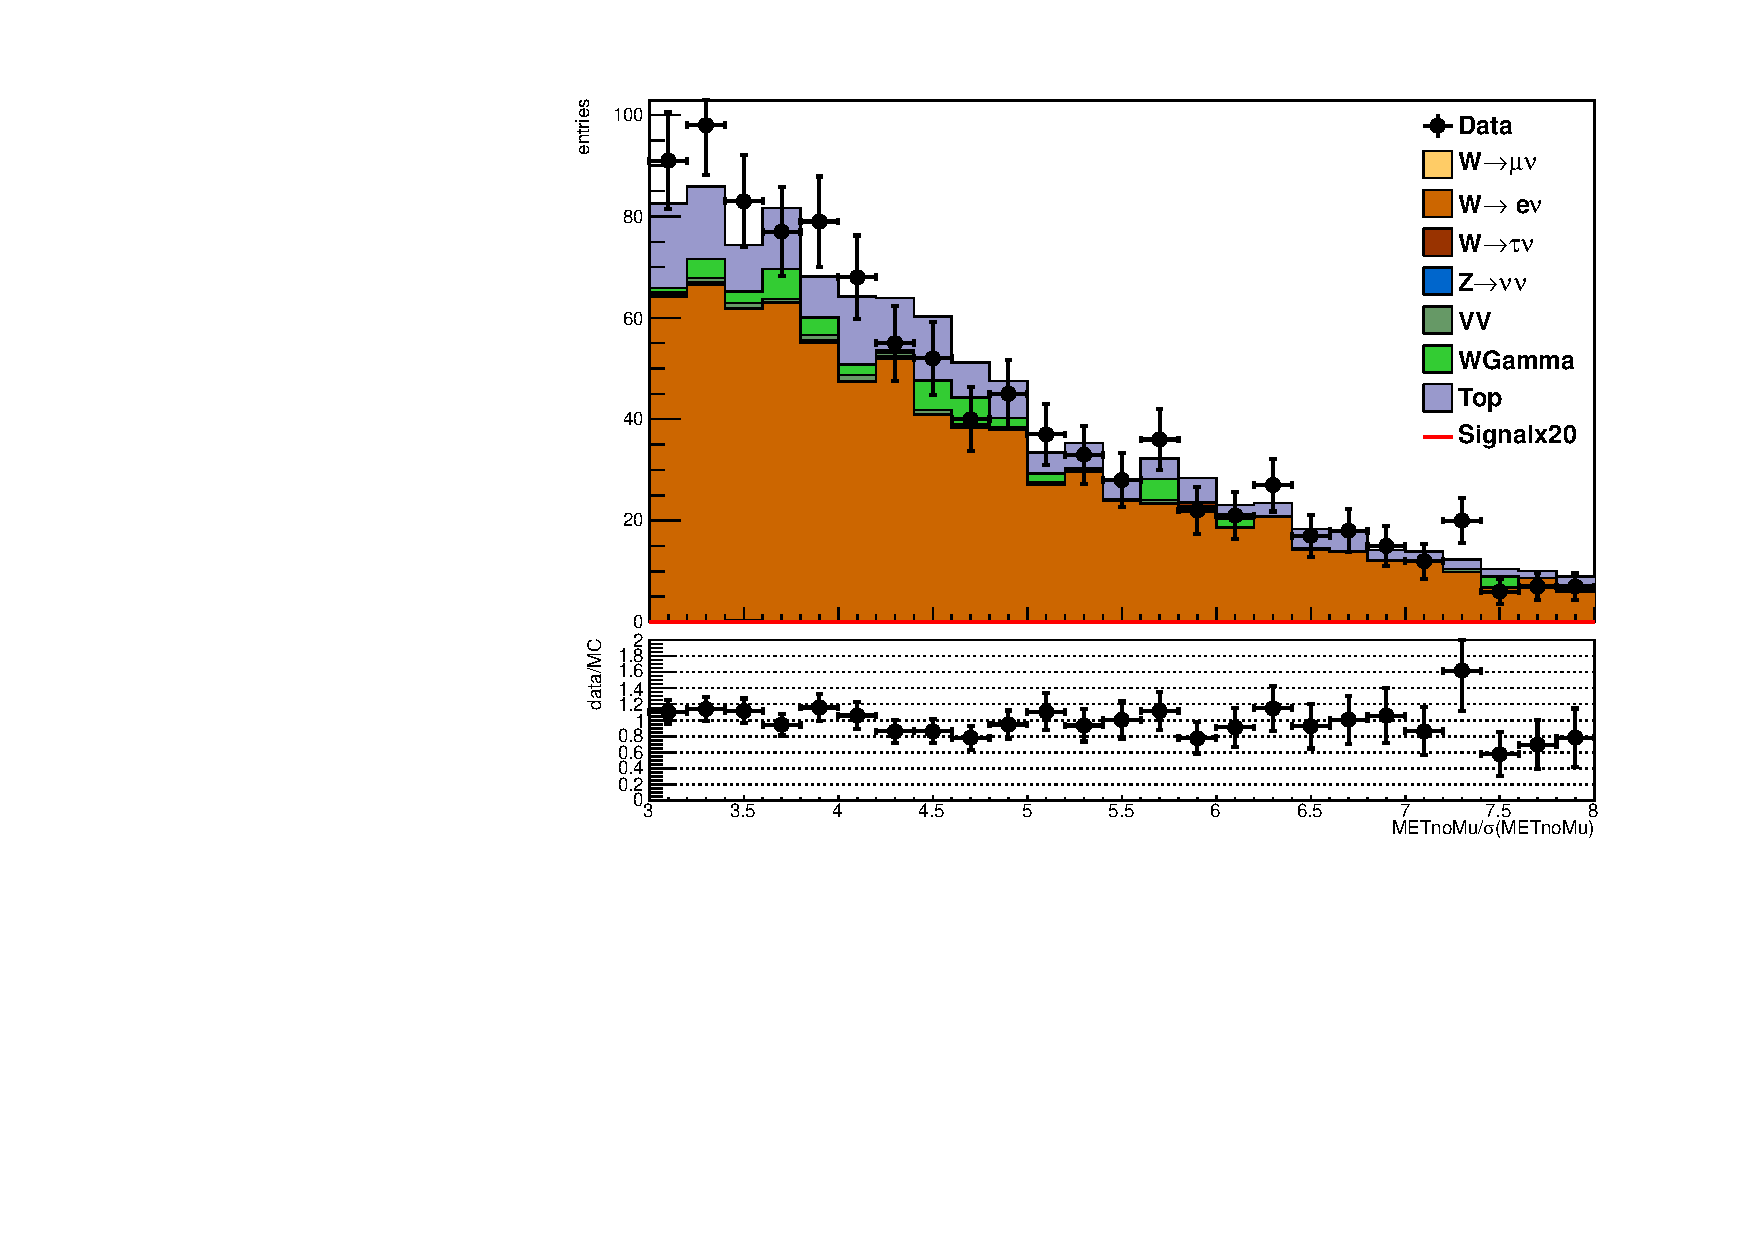
\includegraphics[width=\textwidth]{TalkPics/contplotsandpresel220914/output_contplots_rebinned2dweights/enu_metnomu_significance.pdf}
    \end{block}

  \end{columns}
\end{frame}

\begin{frame}
  \frametitle{New control plots - enu}
  \begin{columns}
    \column{.5\textwidth}
    \begin{block}{Mjj}
      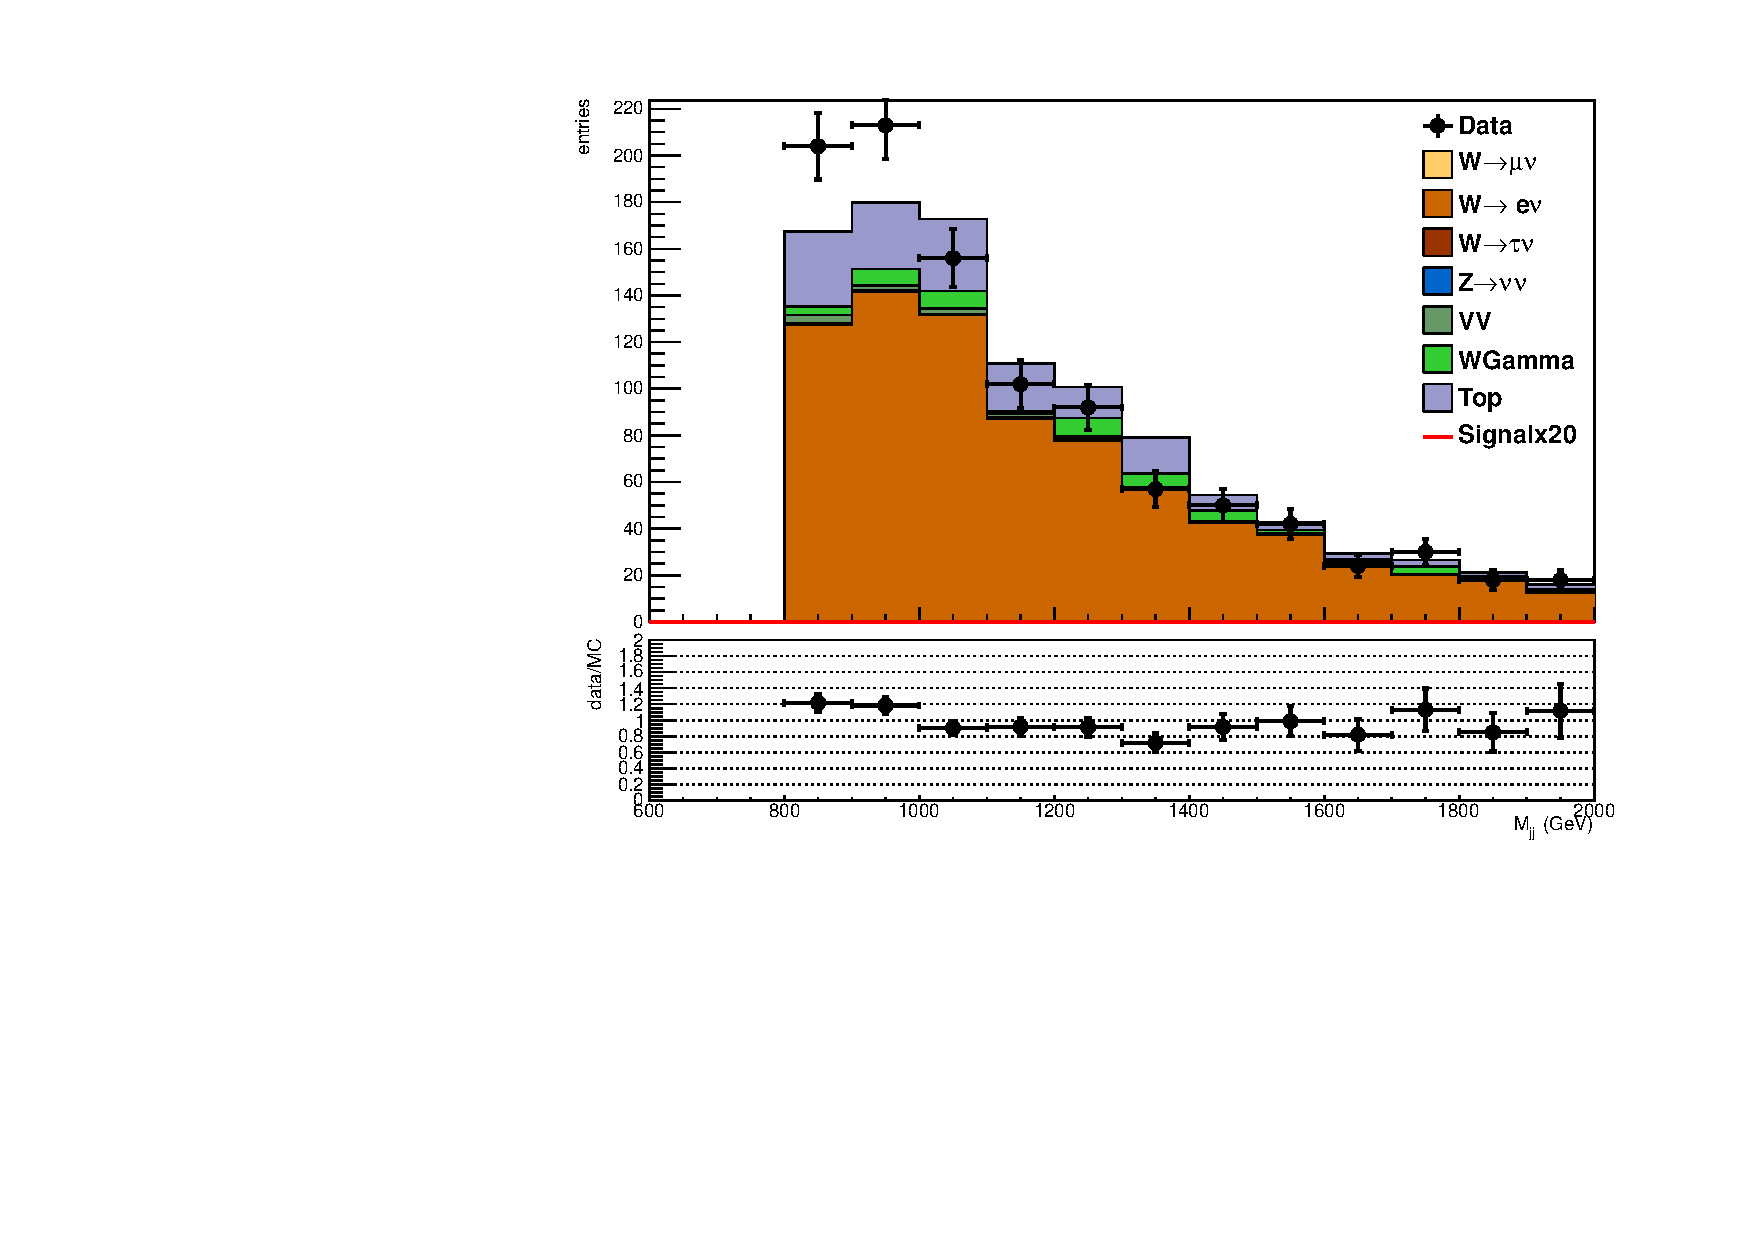
\includegraphics[width=\textwidth]{TalkPics/contplotsandpresel220914/output_contplots_rebinned2dweights/enu_dijet_M.pdf}
    \end{block}
    \column{.5\textwidth}
    \begin{block}{mt}
      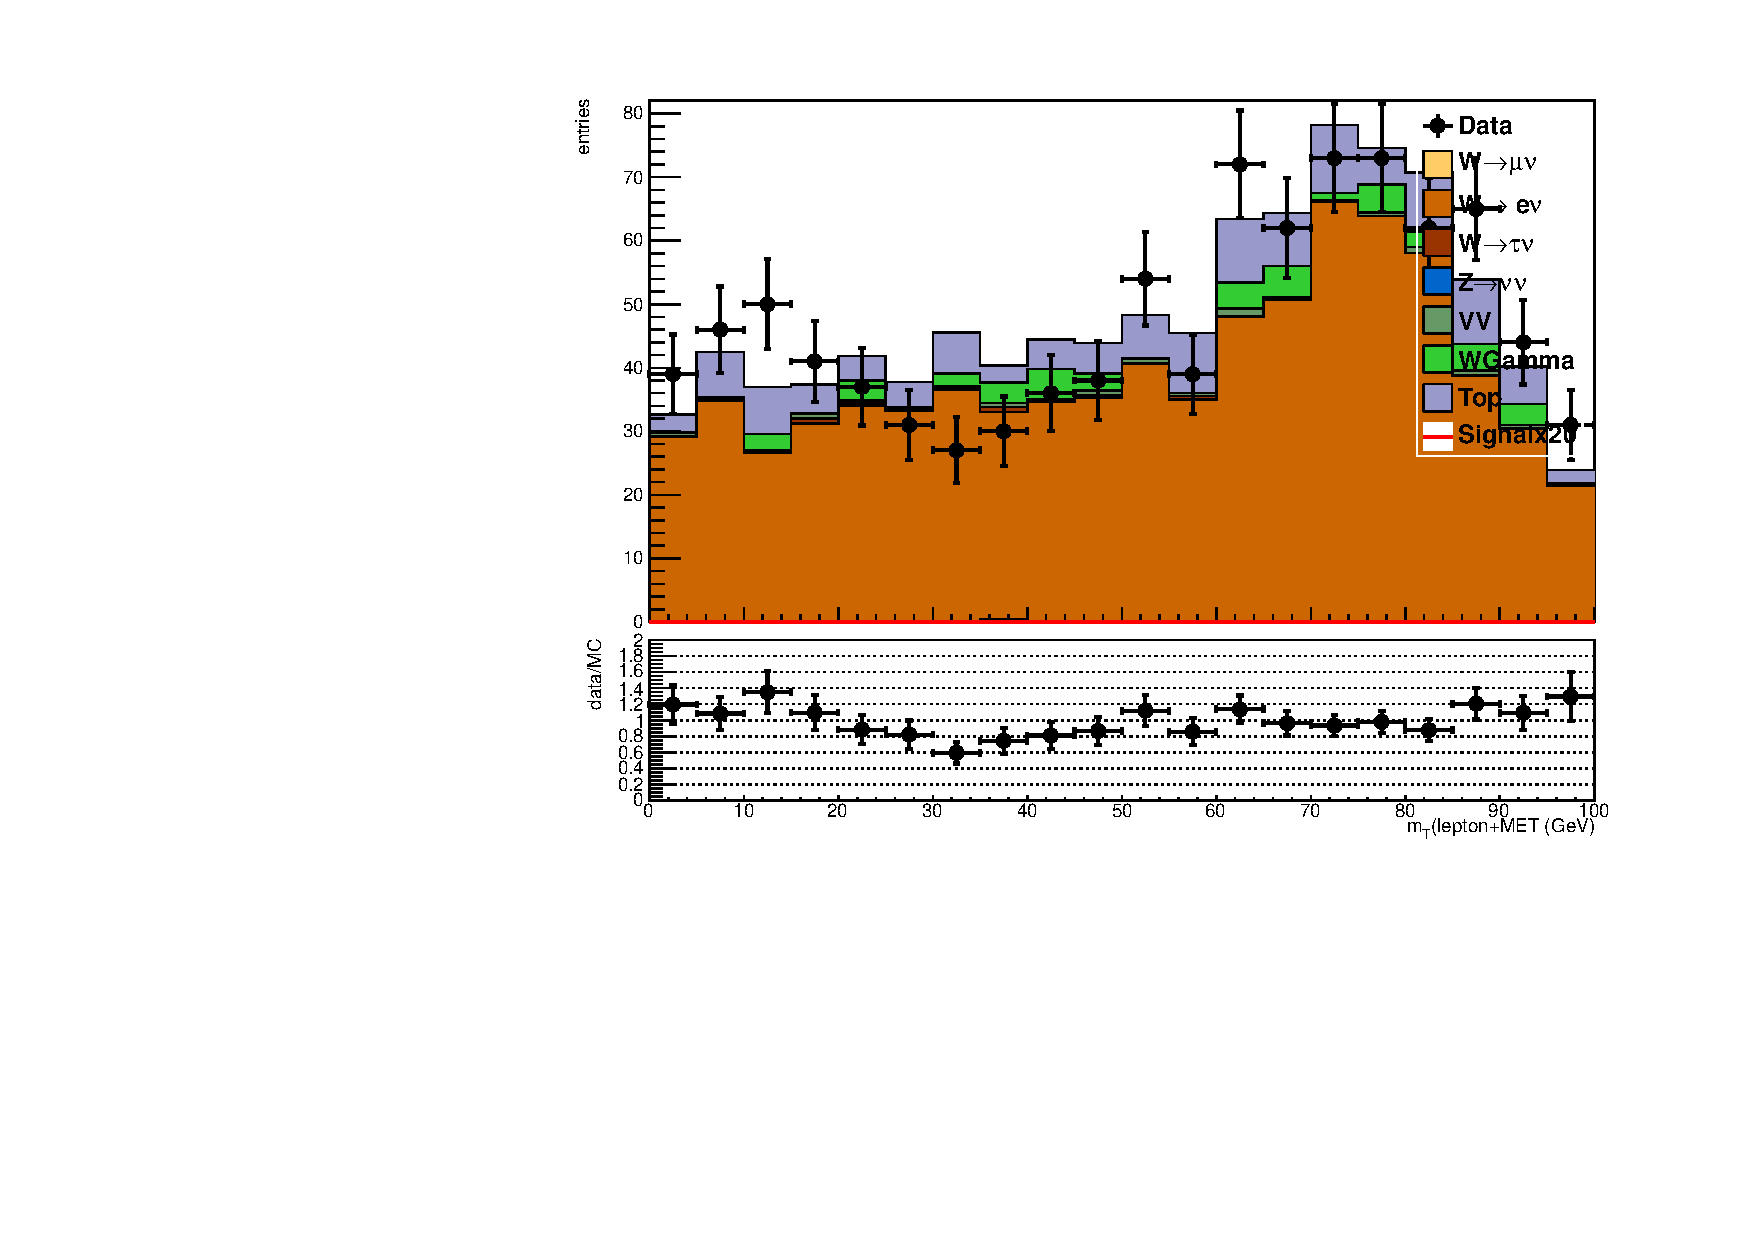
\includegraphics[width=\textwidth]{TalkPics/contplotsandpresel220914/output_contplots_rebinned2dweights/enu_lep_mt.pdf}
    \end{block}
  \end{columns}
\end{frame}

\begin{frame}
  \frametitle{New control plots - enu}
  \begin{columns}
    \column{.5\textwidth}
    \begin{block}{Dijet Dphi}
      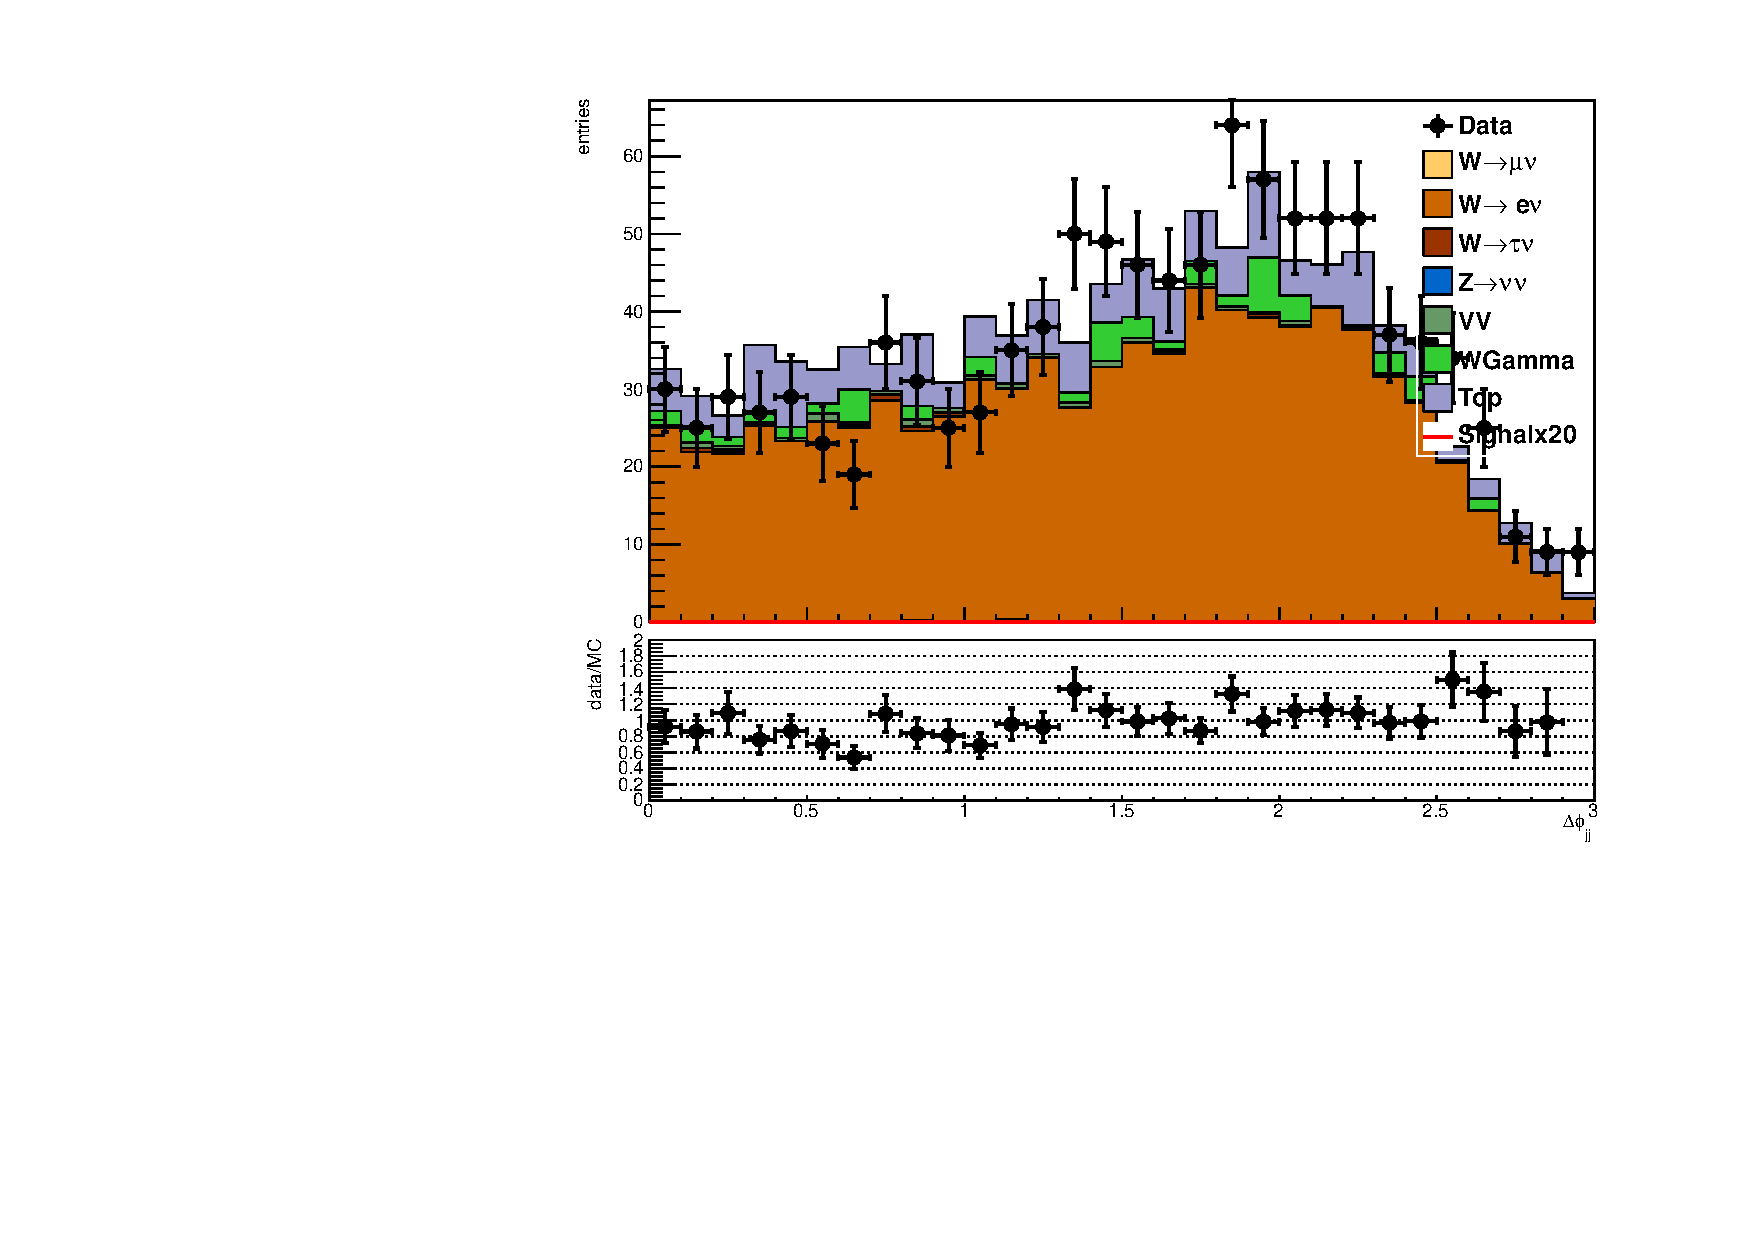
\includegraphics[width=\textwidth]{TalkPics/contplotsandpresel220914/output_contplots_rebinned2dweights/enu_dijet_dphi.pdf}
    \end{block}
    \column{.5\textwidth}
    \begin{block}{Detajj}
      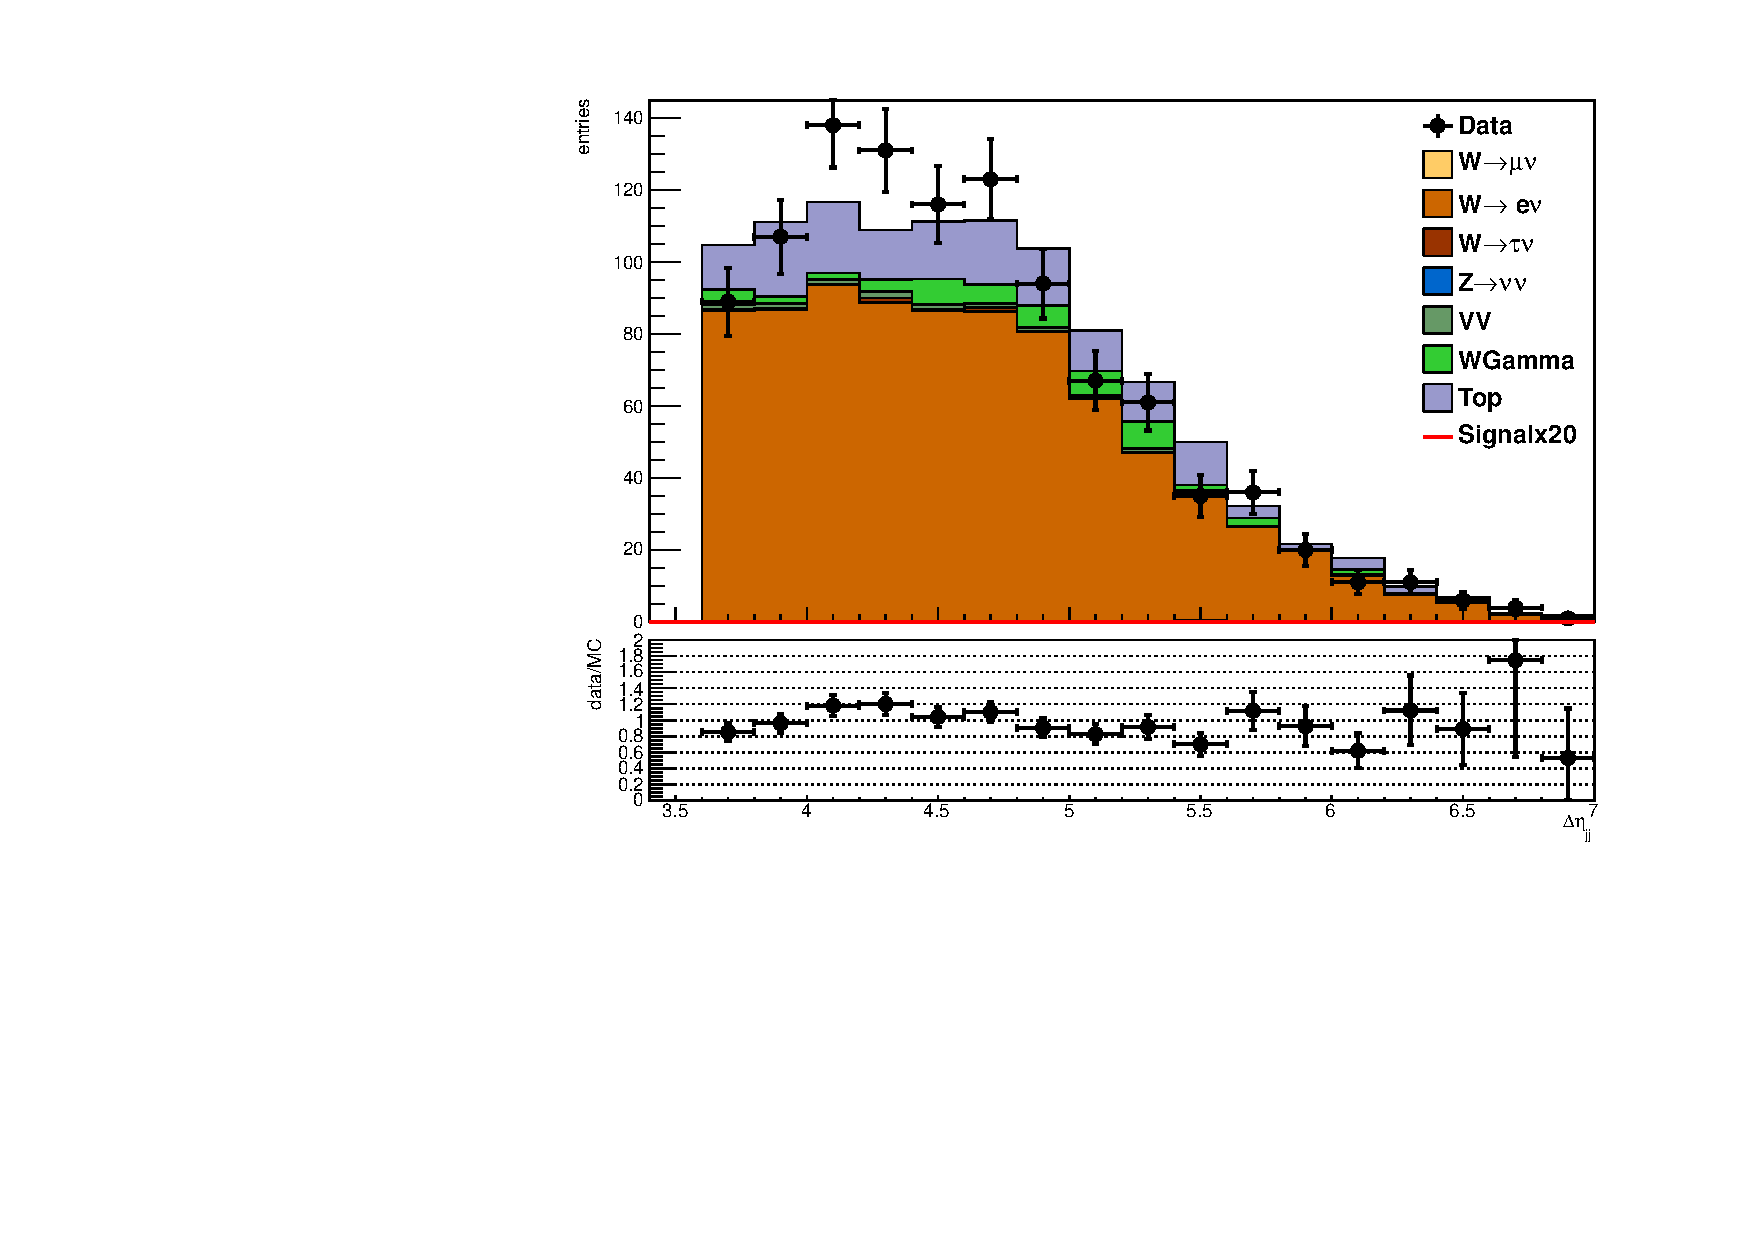
\includegraphics[width=\textwidth]{TalkPics/contplotsandpresel220914/output_contplots_rebinned2dweights/enu_dijet_deta.pdf}
    \end{block}

  \end{columns}
\end{frame}

\begin{frame}
  \frametitle{New control plots - enu}
  \begin{columns}
    \column{.5\textwidth}
    \begin{block}{Leading jets-met mindphi}
      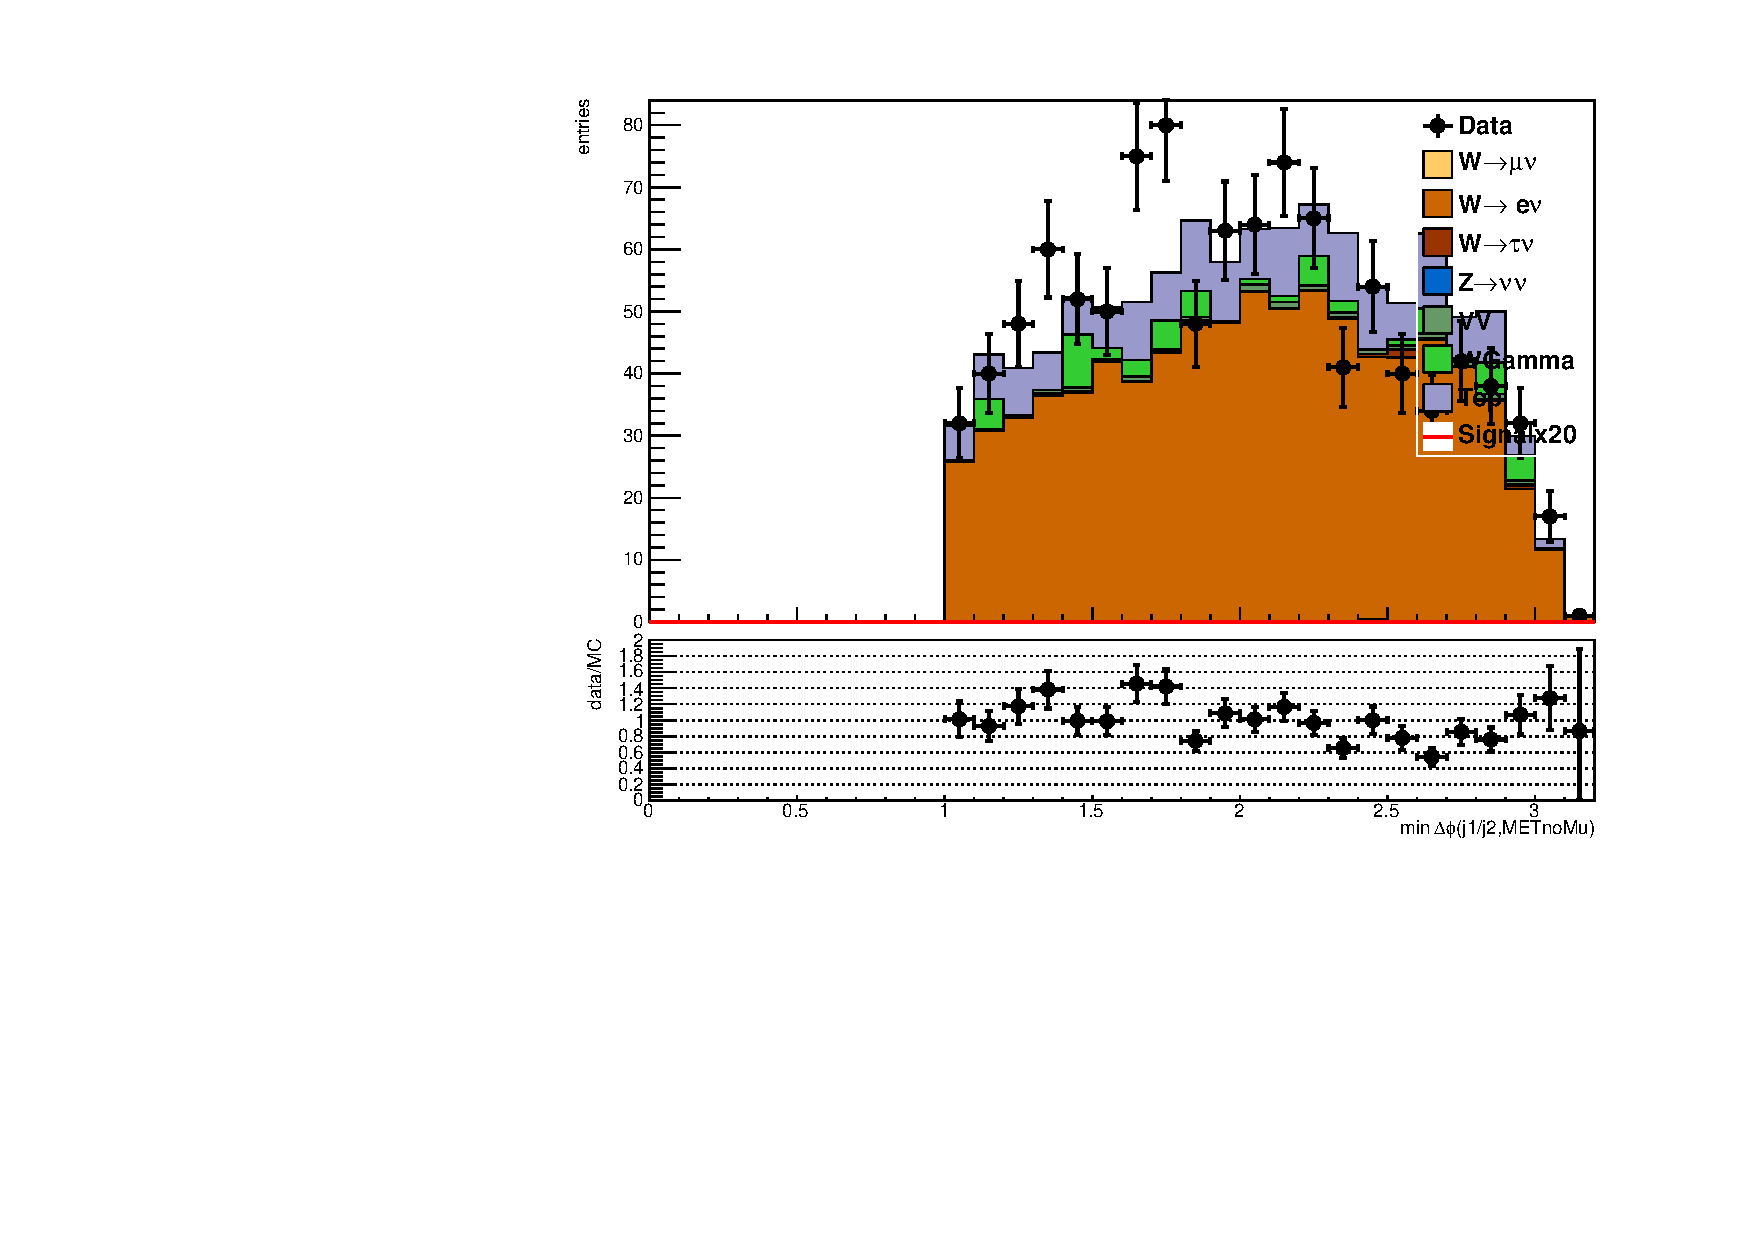
\includegraphics[width=\textwidth]{TalkPics/contplotsandpresel220914/output_contplots_rebinned2dweights/enu_jetmetnomu_mindphi.pdf}
    \end{block}
    \column{.5\textwidth}
    \begin{block}{All jets-met mindphi}
      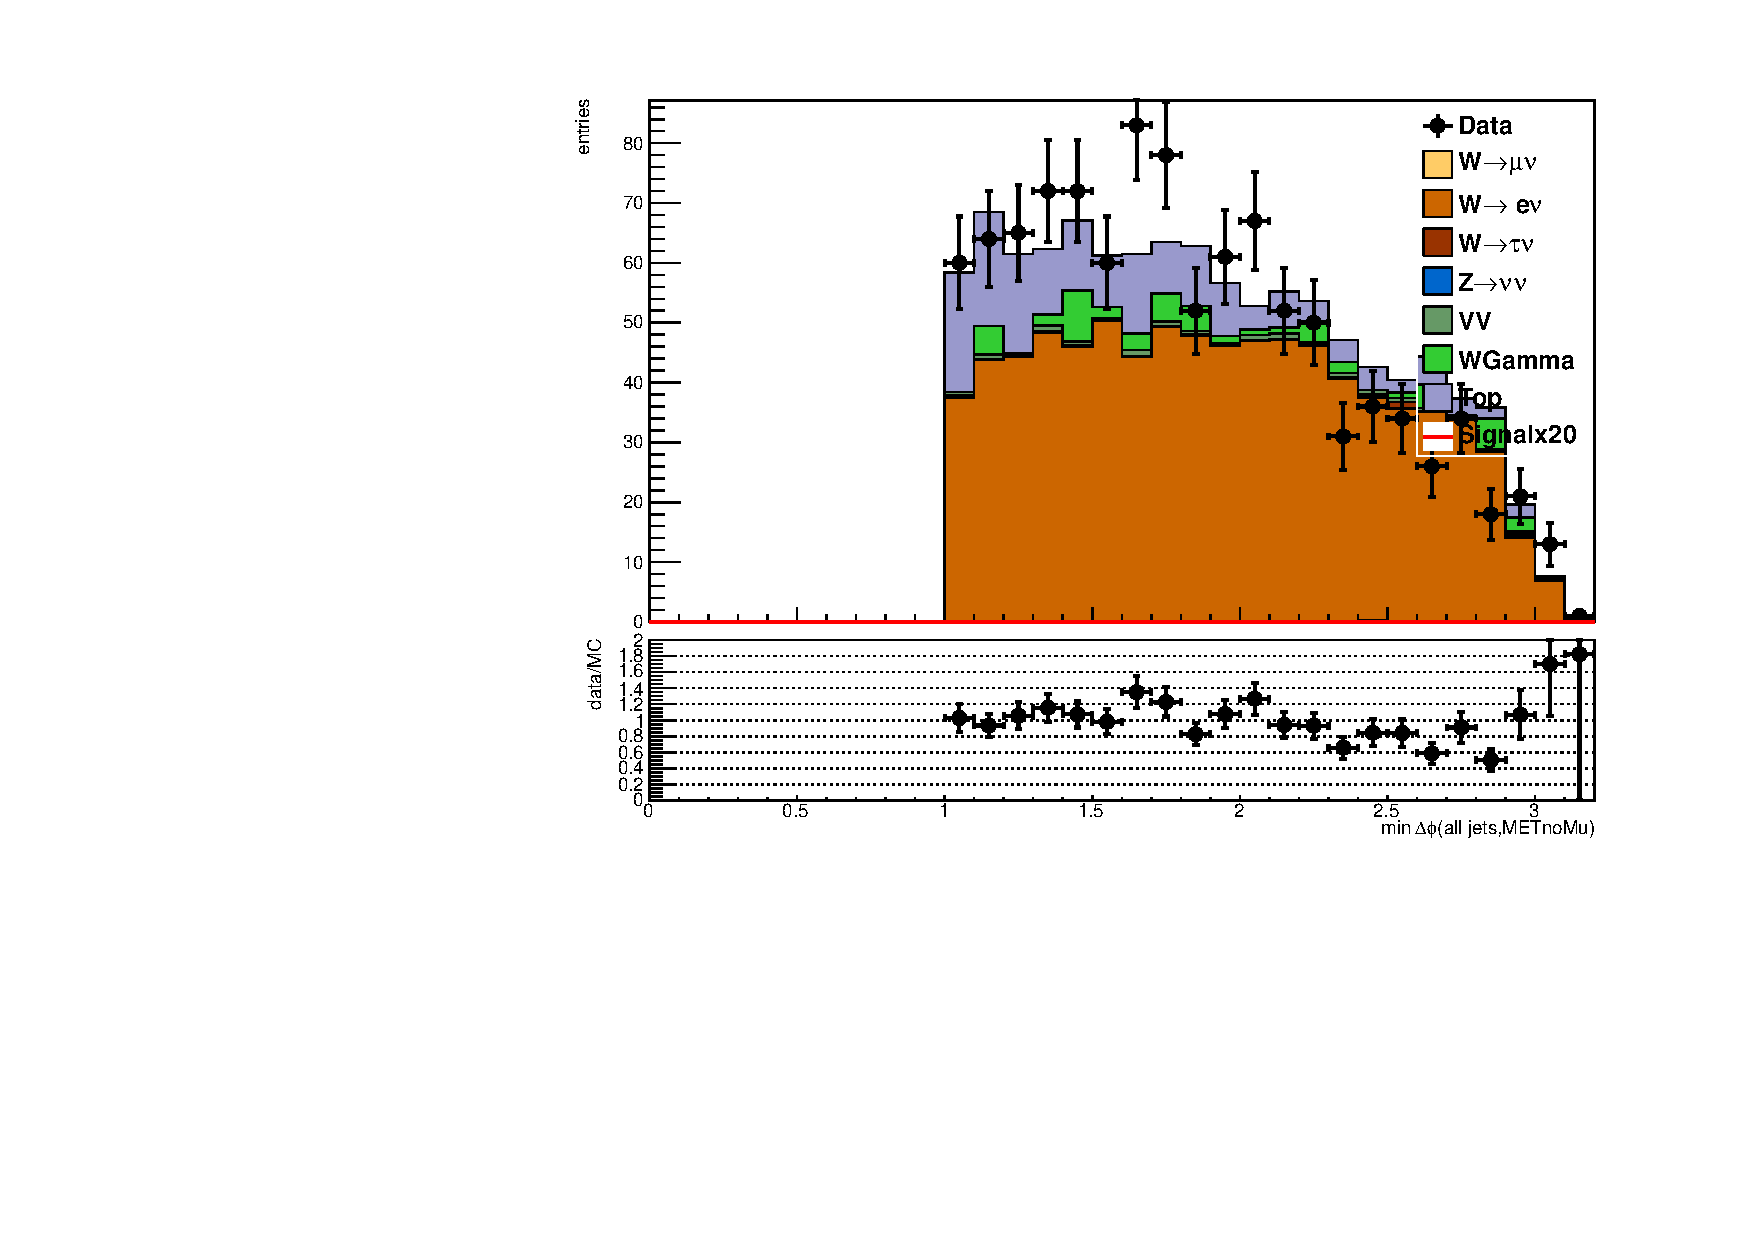
\includegraphics[width=\textwidth]{TalkPics/contplotsandpresel220914/output_contplots_rebinned2dweights/enu_alljetsmetnomu_mindphi.pdf}
    \end{block}

  \end{columns}
\end{frame}

\begin{frame}
  \frametitle{New control plots - enu}
  \begin{columns}
    \column{.5\textwidth}
    \begin{block}{dijet-metnomu pt fraction}
      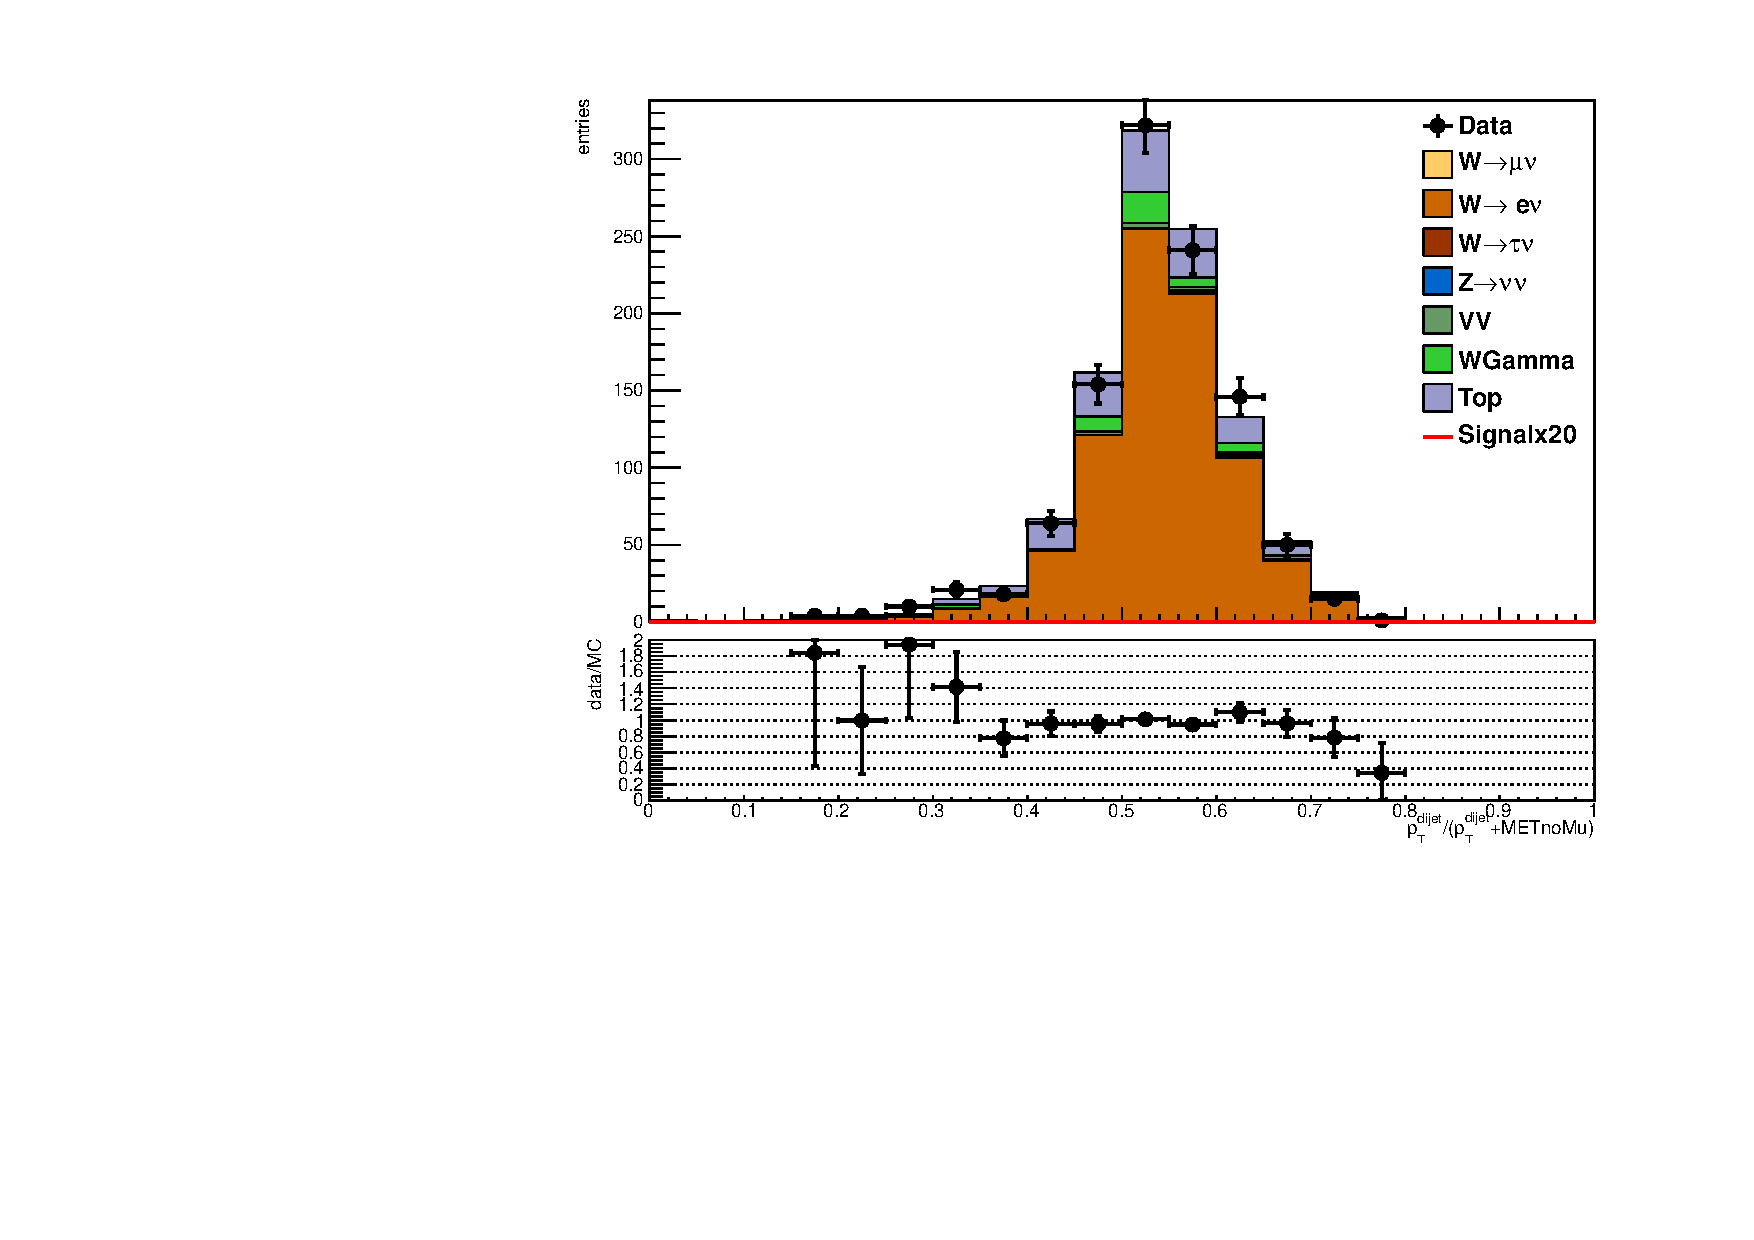
\includegraphics[width=\textwidth]{TalkPics/contplotsandpresel220914/output_contplots_rebinned2dweights/enu_dijetmetnomu_ptfraction.pdf}
    \end{block}
  \end{columns}
\end{frame}

\begin{frame}
  \frametitle{New control plots - munu}
  \begin{columns}
    \column{.5\textwidth}
    \begin{block}{Jet 1 pt}
      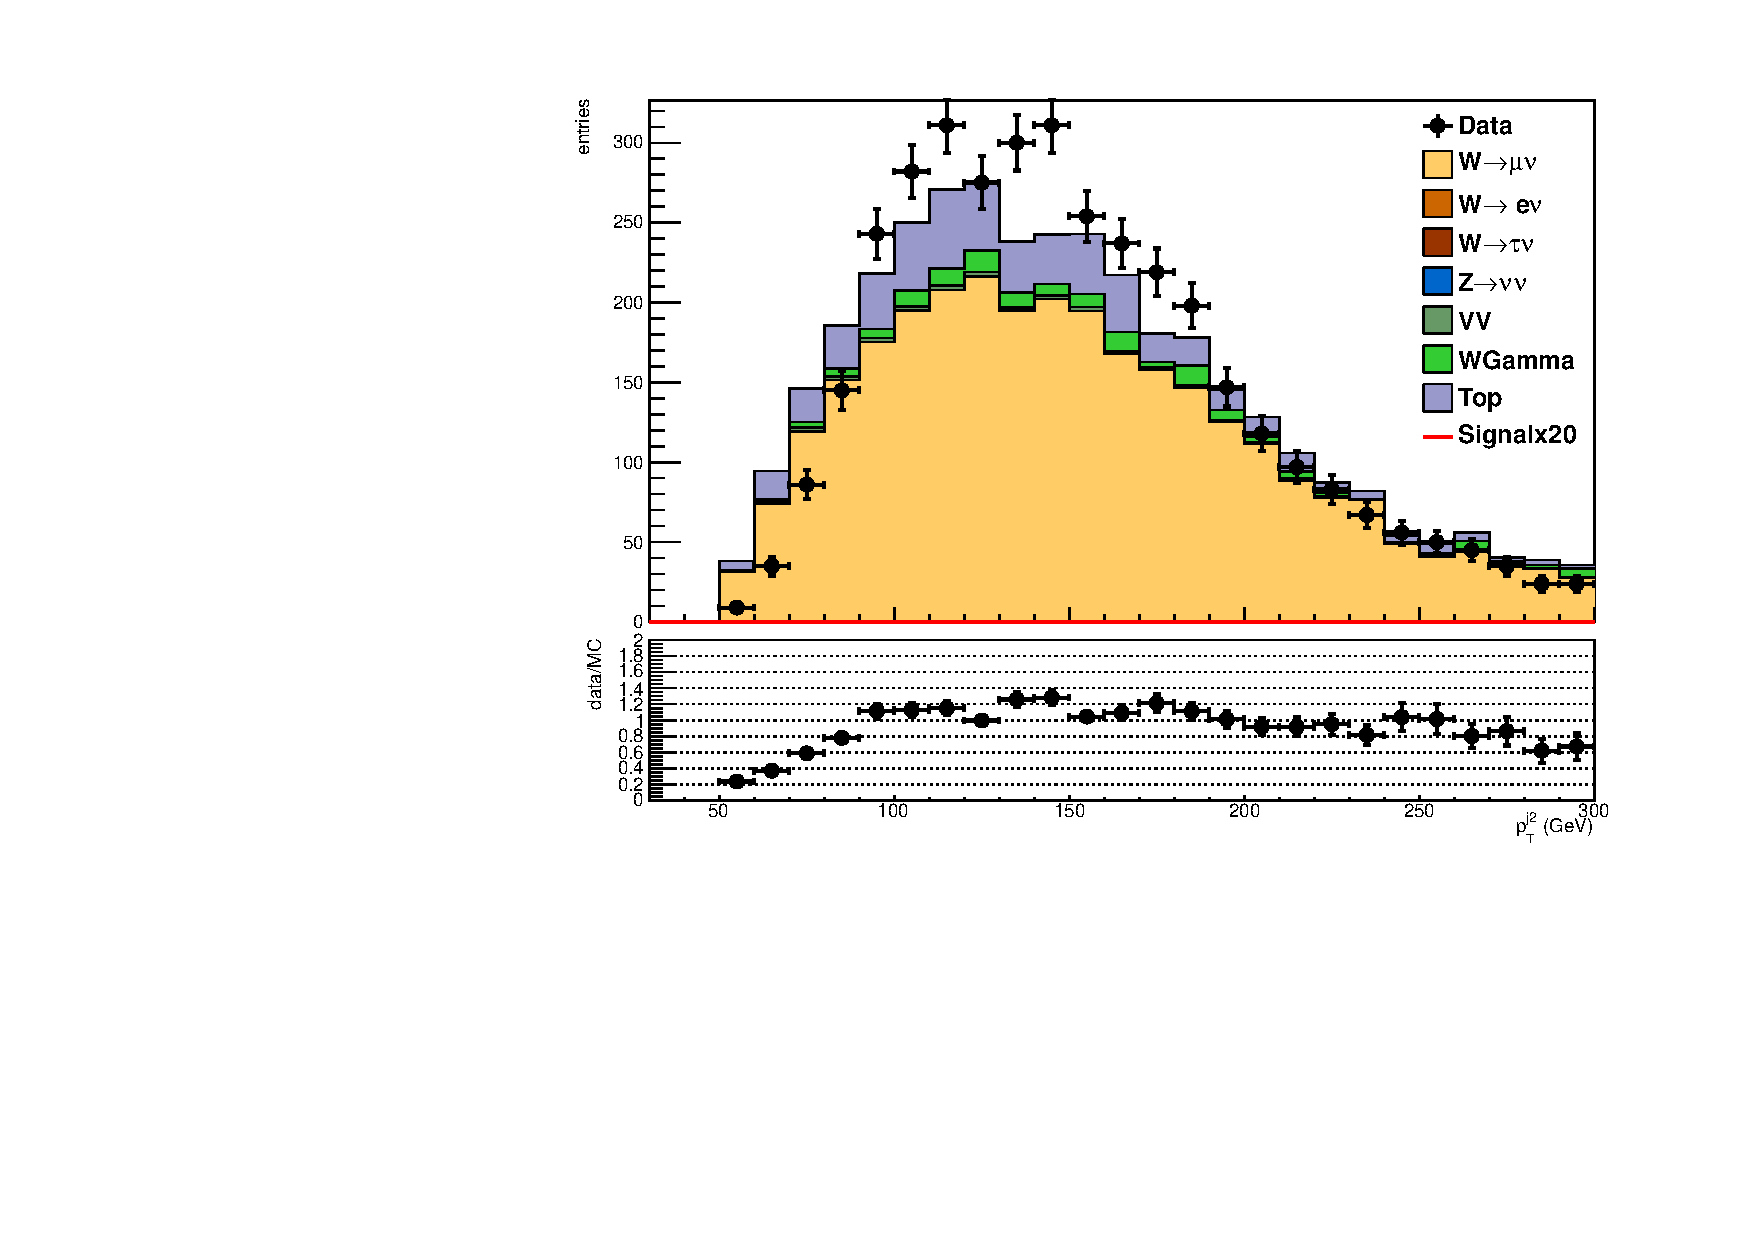
\includegraphics[width=\textwidth]{TalkPics/contplotsandpresel220914/output_contplots_rebinned2dweights/munu_jet1_pt.pdf}
    \end{block}
    \column{.5\textwidth}
    \begin{block}{Jet 2 pt}
      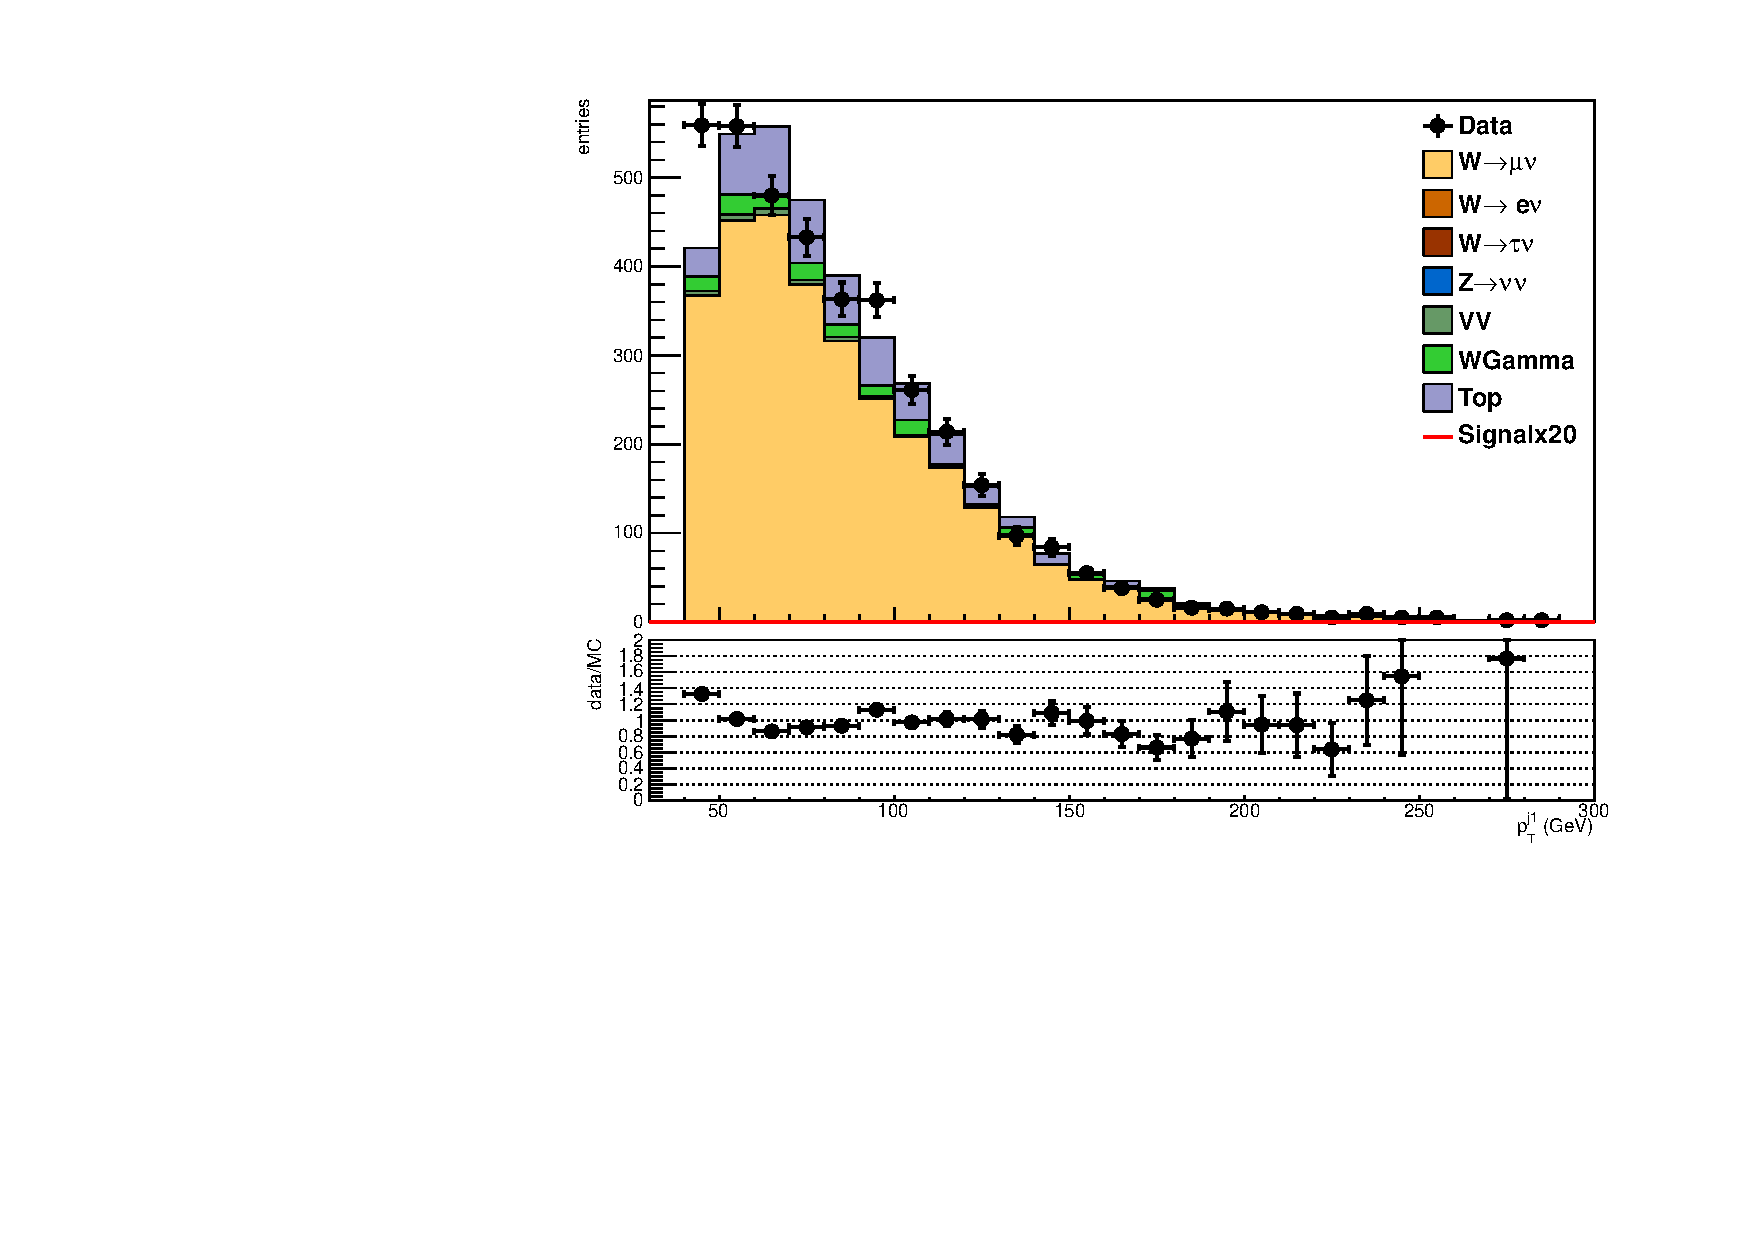
\includegraphics[width=\textwidth]{TalkPics/contplotsandpresel220914/output_contplots_rebinned2dweights/munu_jet2_pt.pdf}
    \end{block}

  \end{columns}
\end{frame}

\begin{frame}
  \frametitle{New control plots - munu}
  \begin{columns}
    \column{.5\textwidth}
    \begin{block}{METnomu}
      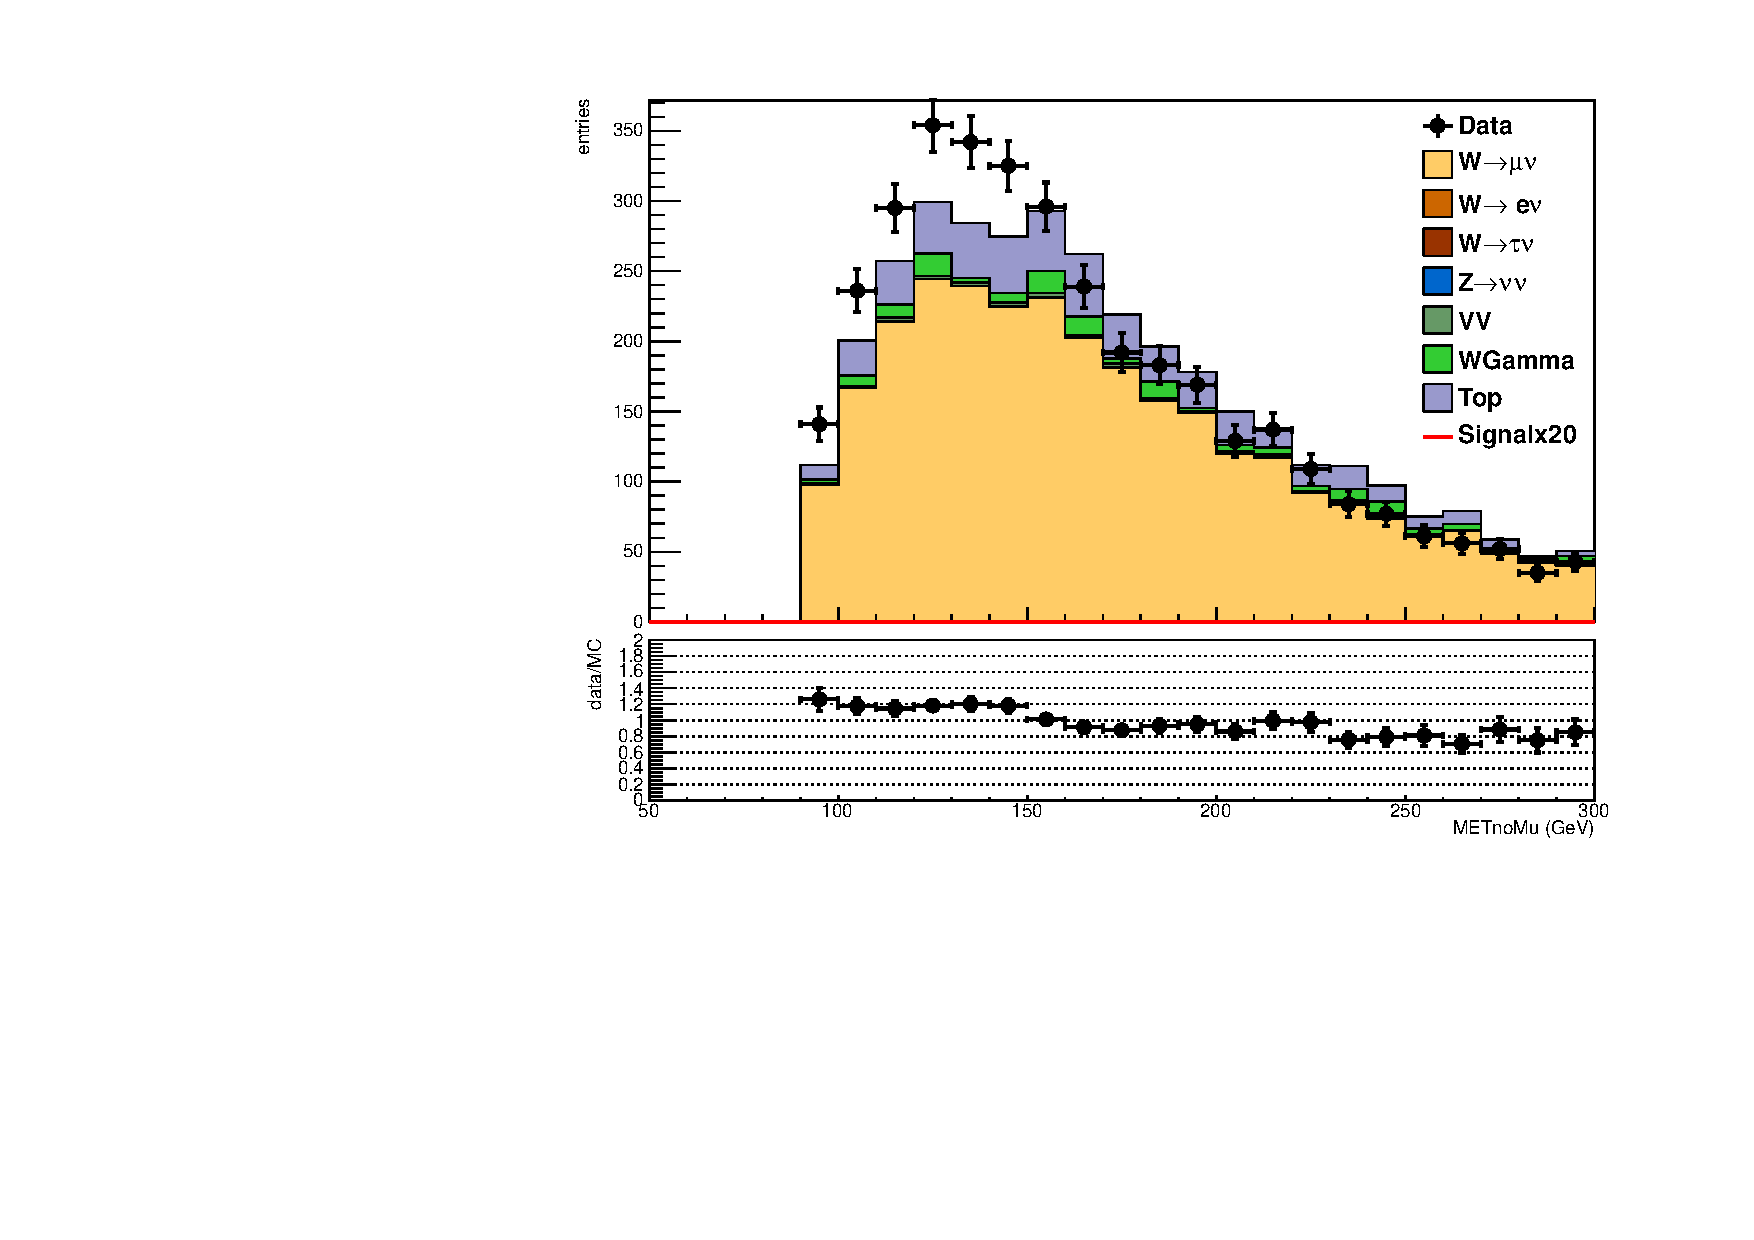
\includegraphics[width=\textwidth]{TalkPics/contplotsandpresel220914/output_contplots_rebinned2dweights/munu_metnomuons.pdf}
    \end{block}
    \column{.5\textwidth}
    \begin{block}{METnomusig}
      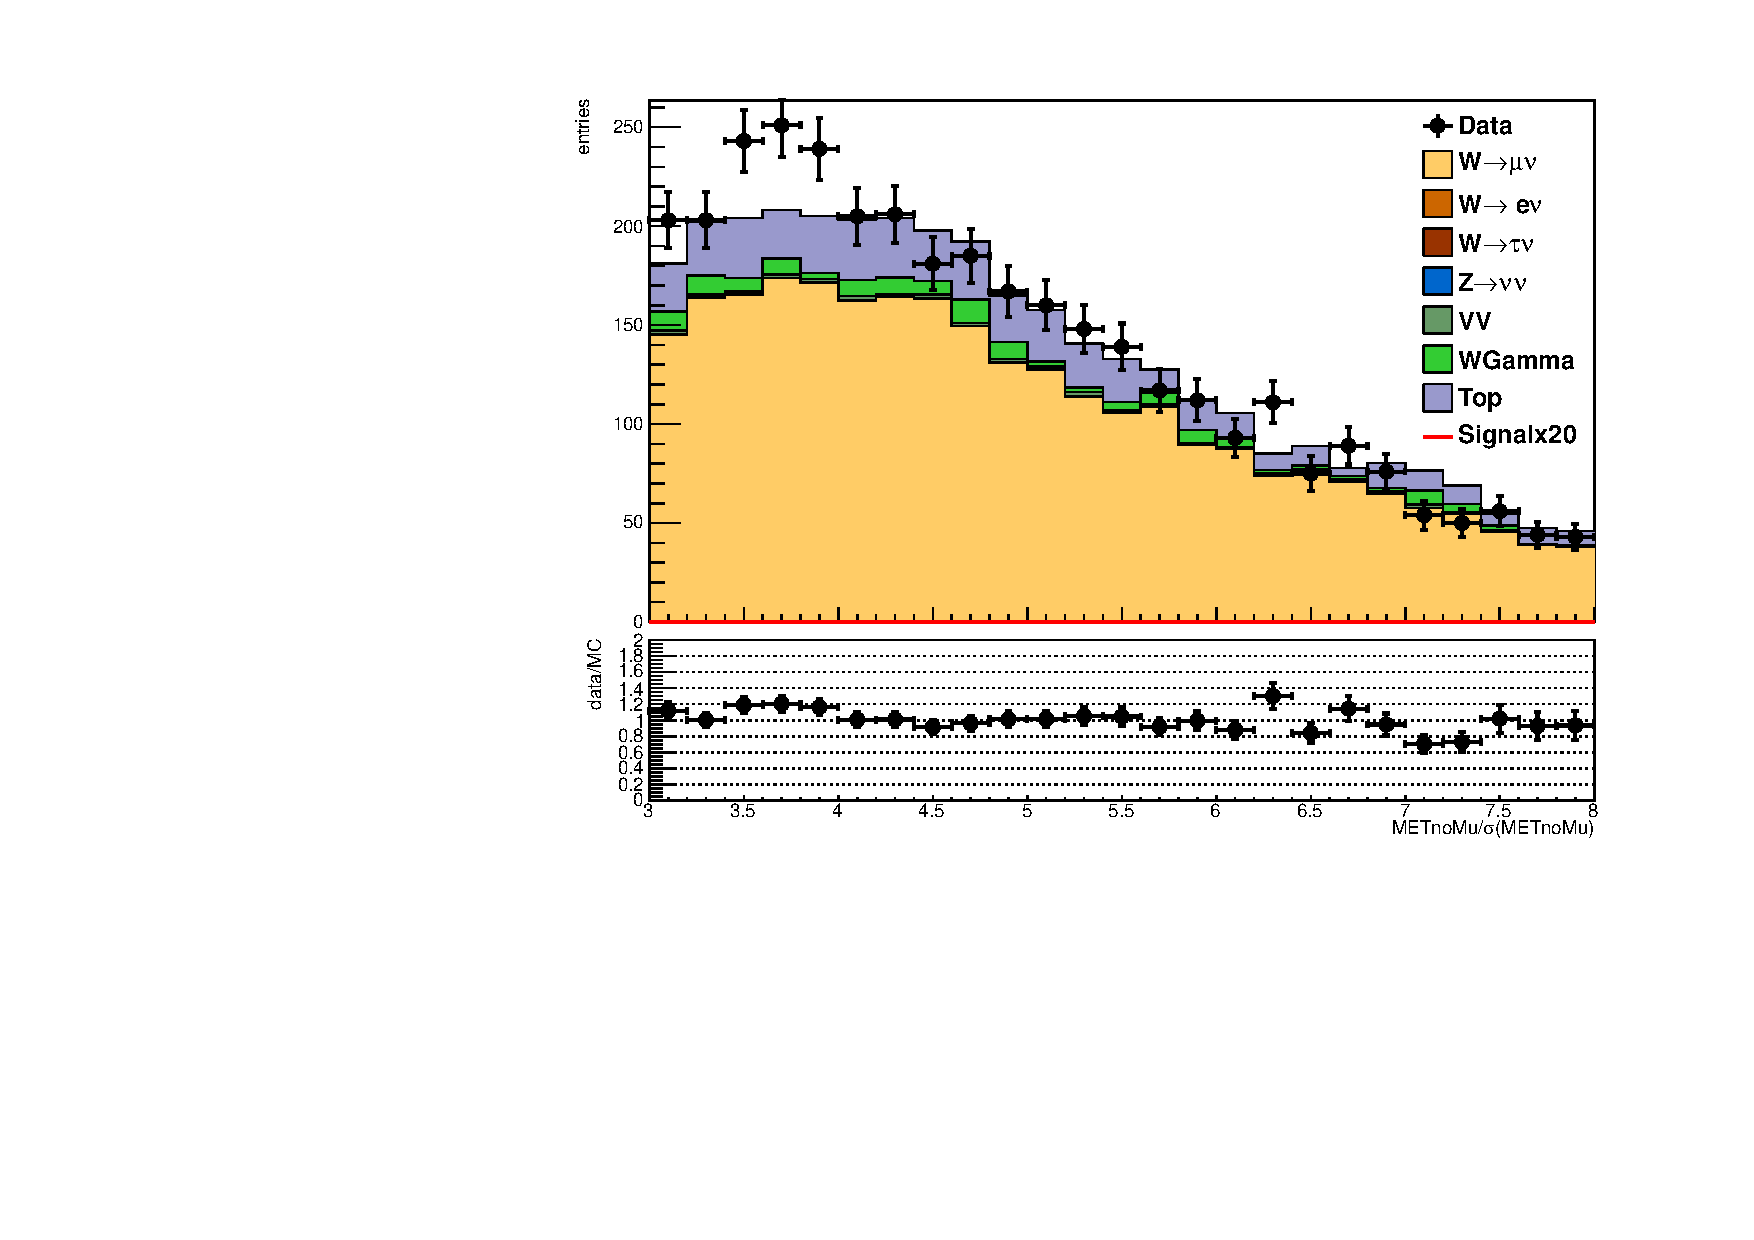
\includegraphics[width=\textwidth]{TalkPics/contplotsandpresel220914/output_contplots_rebinned2dweights/munu_metnomu_significance.pdf}
    \end{block}

  \end{columns}
\end{frame}

\begin{frame}
  \frametitle{New control plots - munu}
  \begin{columns}
    \column{.5\textwidth}
    \begin{block}{Mjj}
      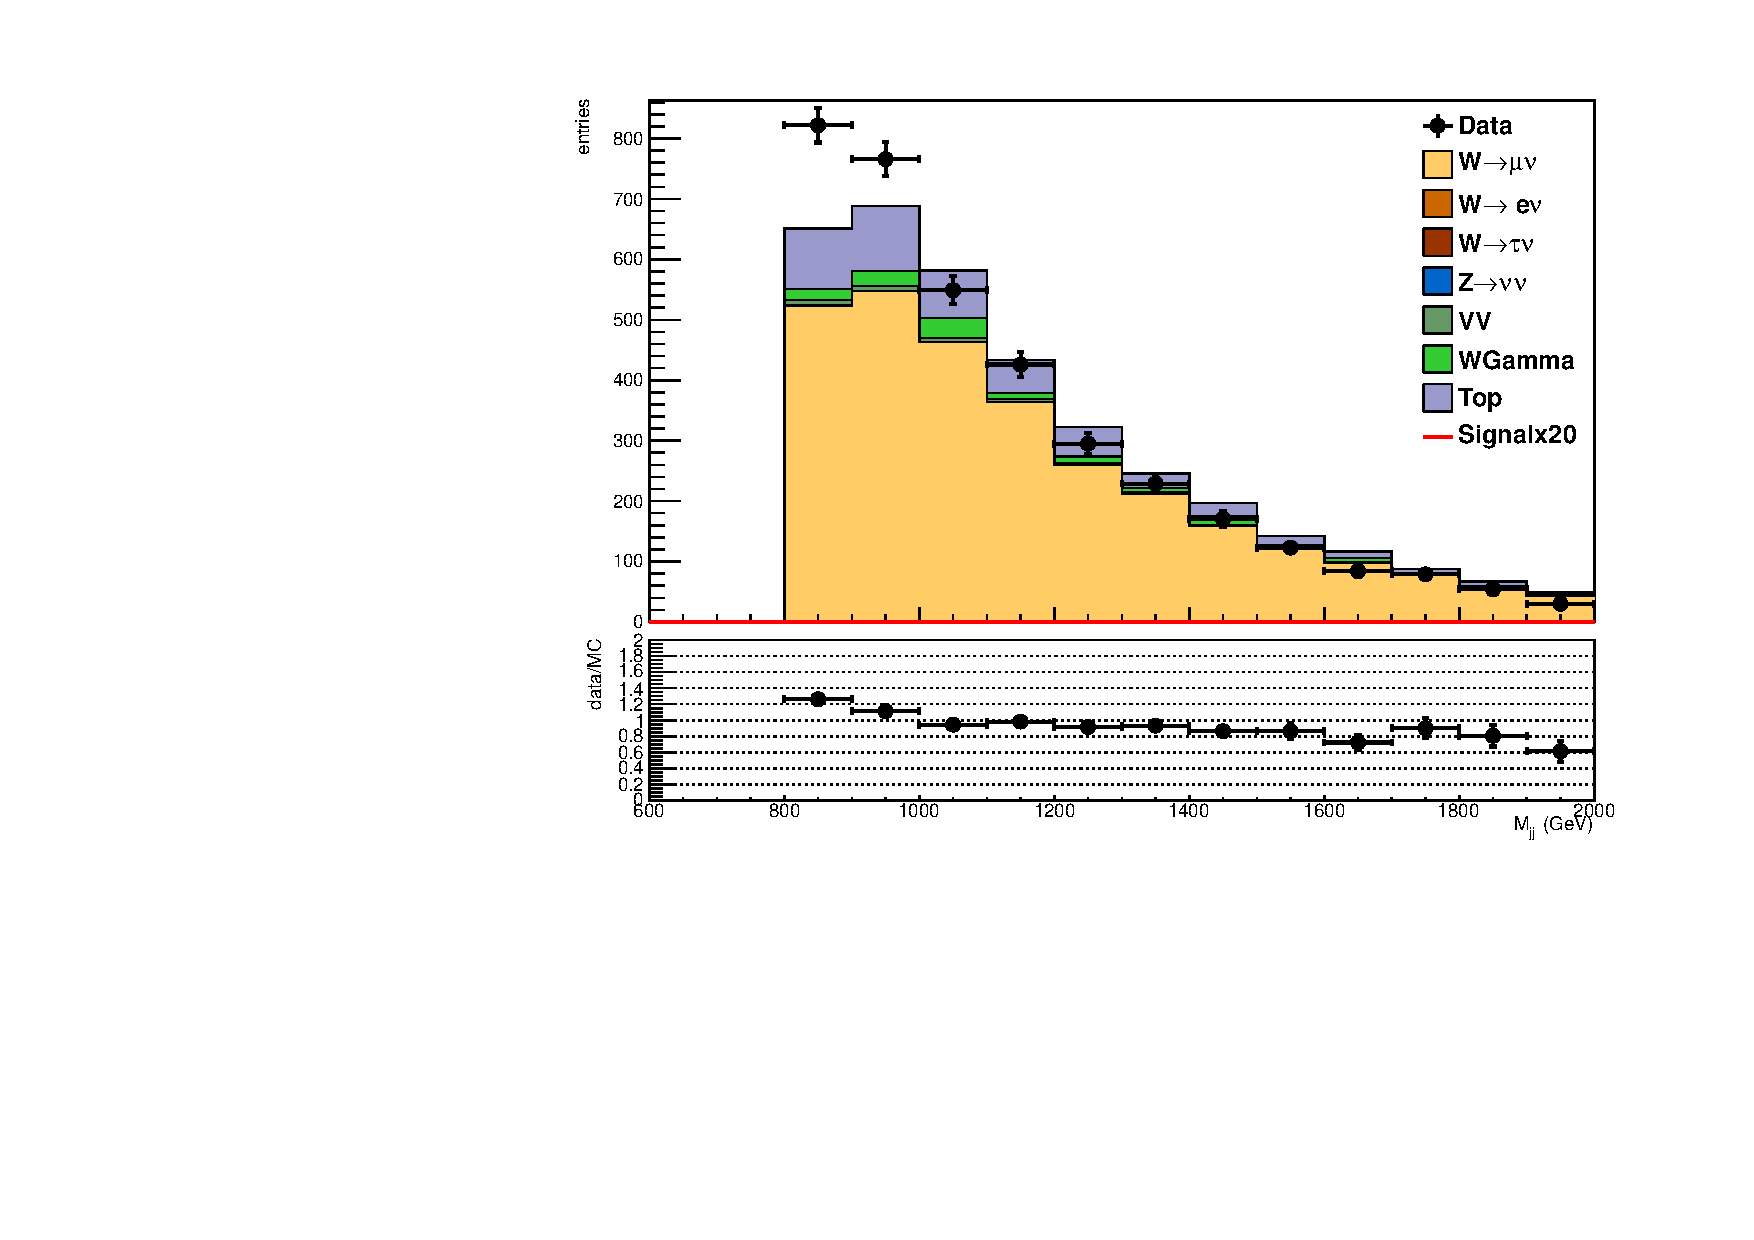
\includegraphics[width=\textwidth]{TalkPics/contplotsandpresel220914/output_contplots_rebinned2dweights/munu_dijet_M.pdf}
    \end{block}
    \column{.5\textwidth}
    \begin{block}{mt}
      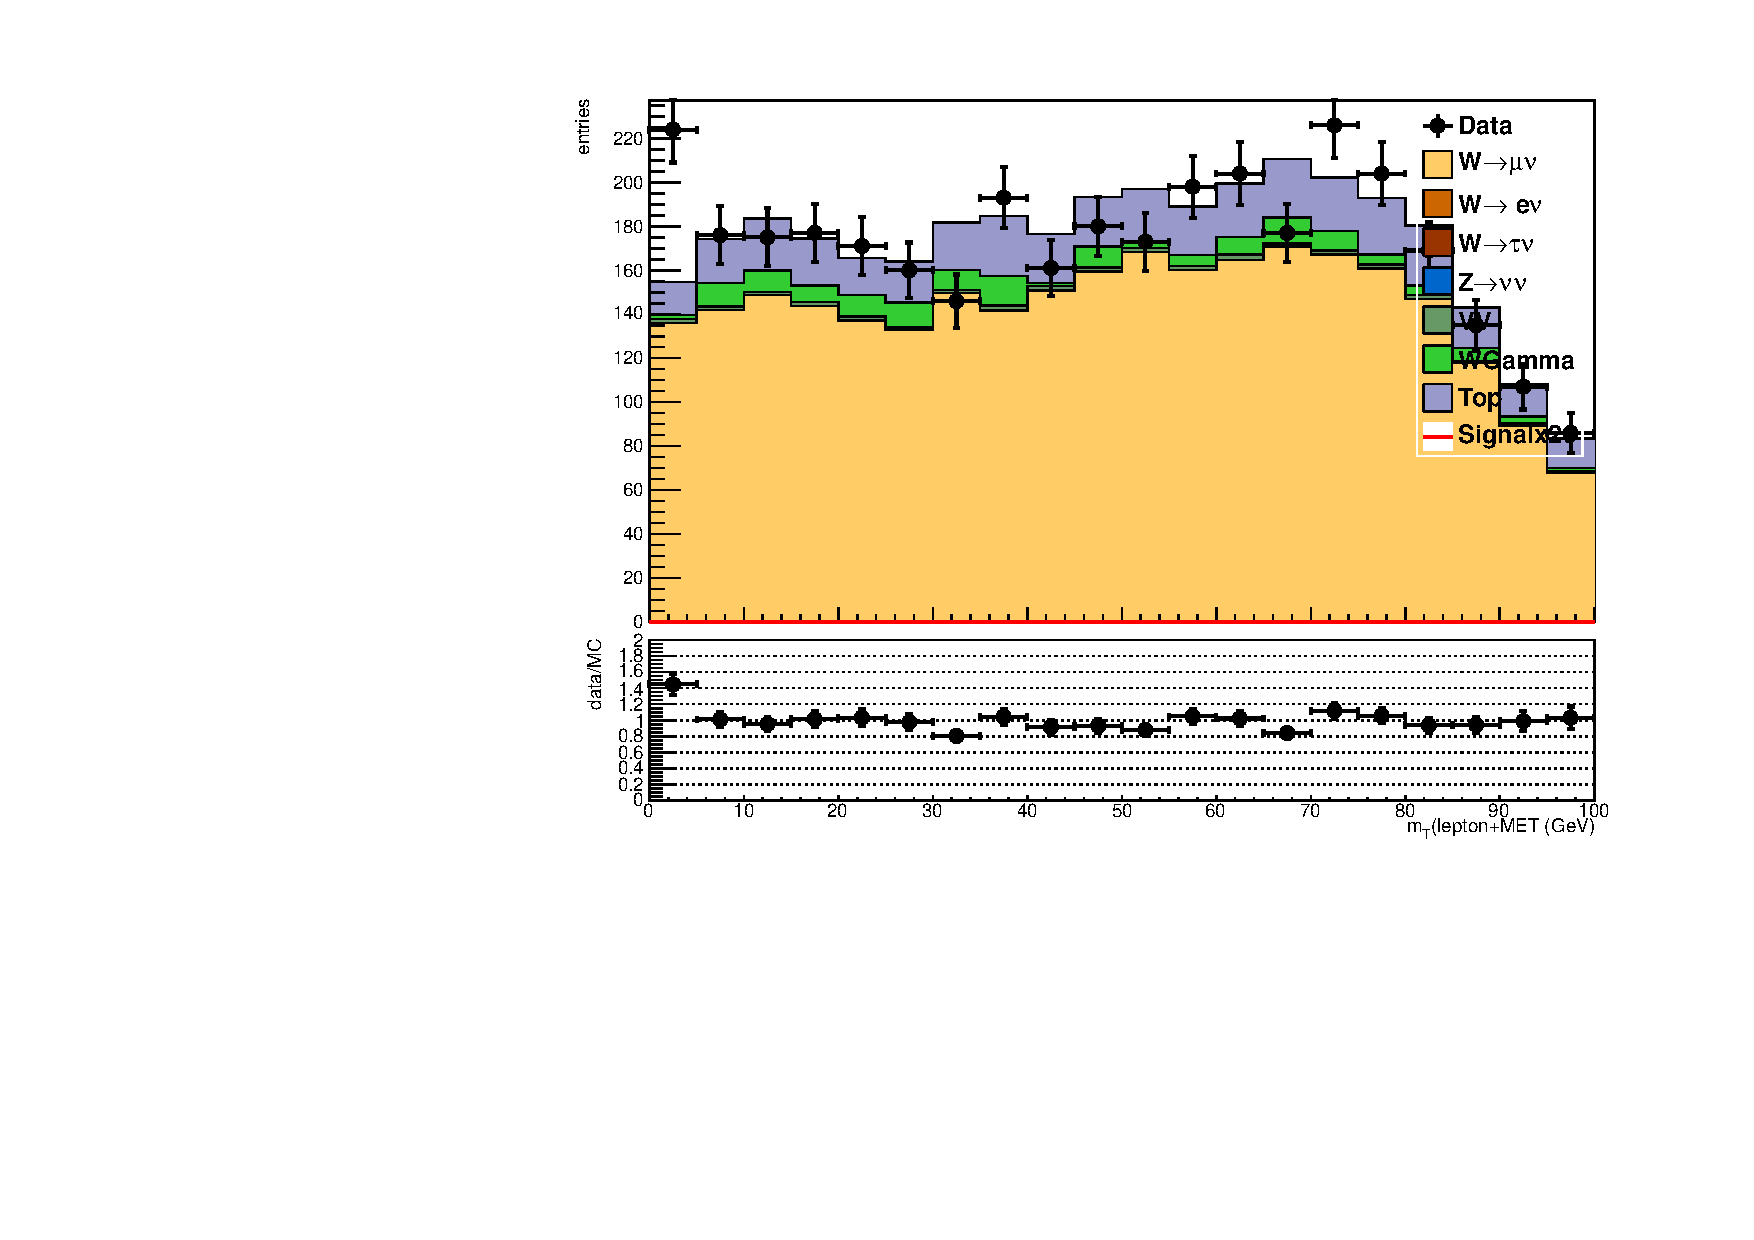
\includegraphics[width=\textwidth]{TalkPics/contplotsandpresel220914/output_contplots_rebinned2dweights/munu_lep_mt.pdf}
    \end{block}
  \end{columns}
\end{frame}

\begin{frame}
  \frametitle{New control plots - munu}
  \begin{columns}
    \column{.5\textwidth}
    \begin{block}{Dijet Dphi}
      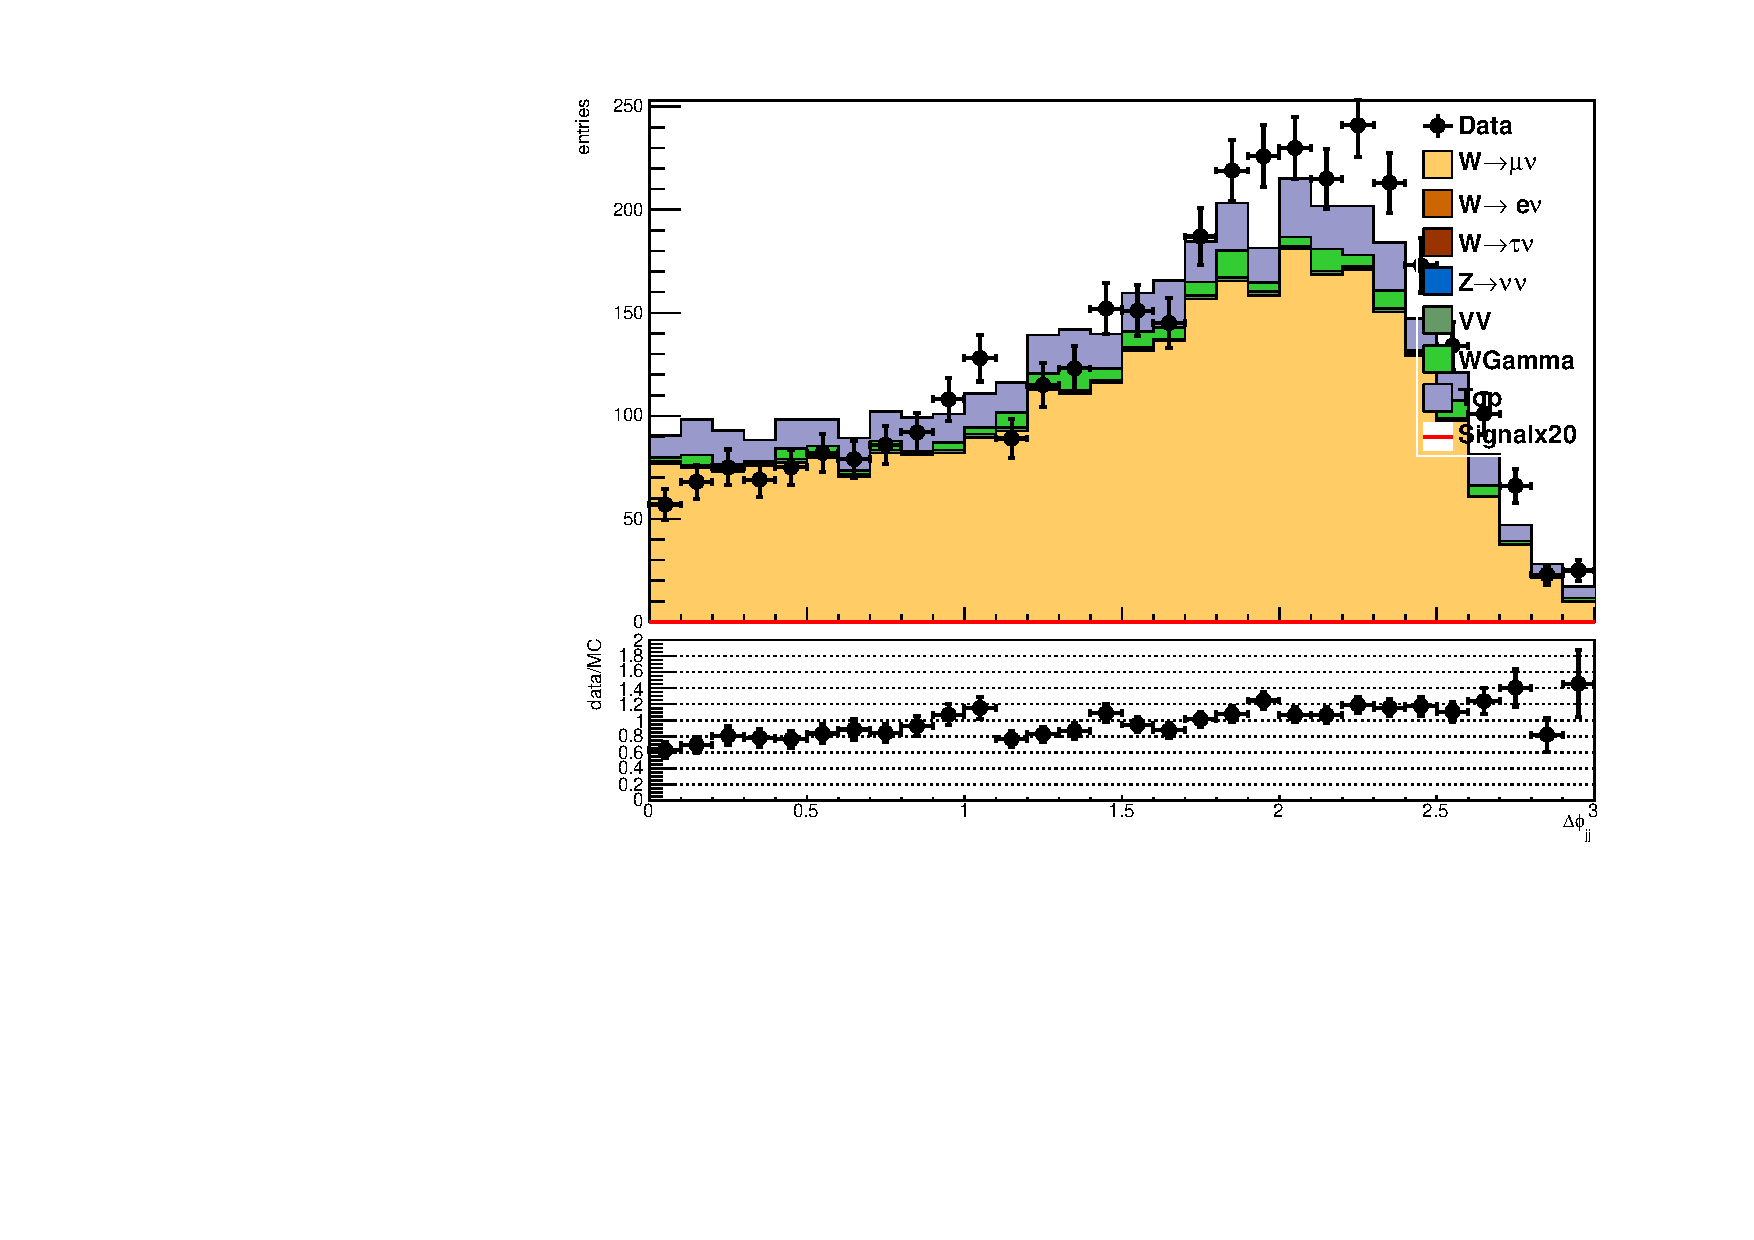
\includegraphics[width=\textwidth]{TalkPics/contplotsandpresel220914/output_contplots_rebinned2dweights/munu_dijet_dphi.pdf}
    \end{block}
    \column{.5\textwidth}
    \begin{block}{Detajj}
      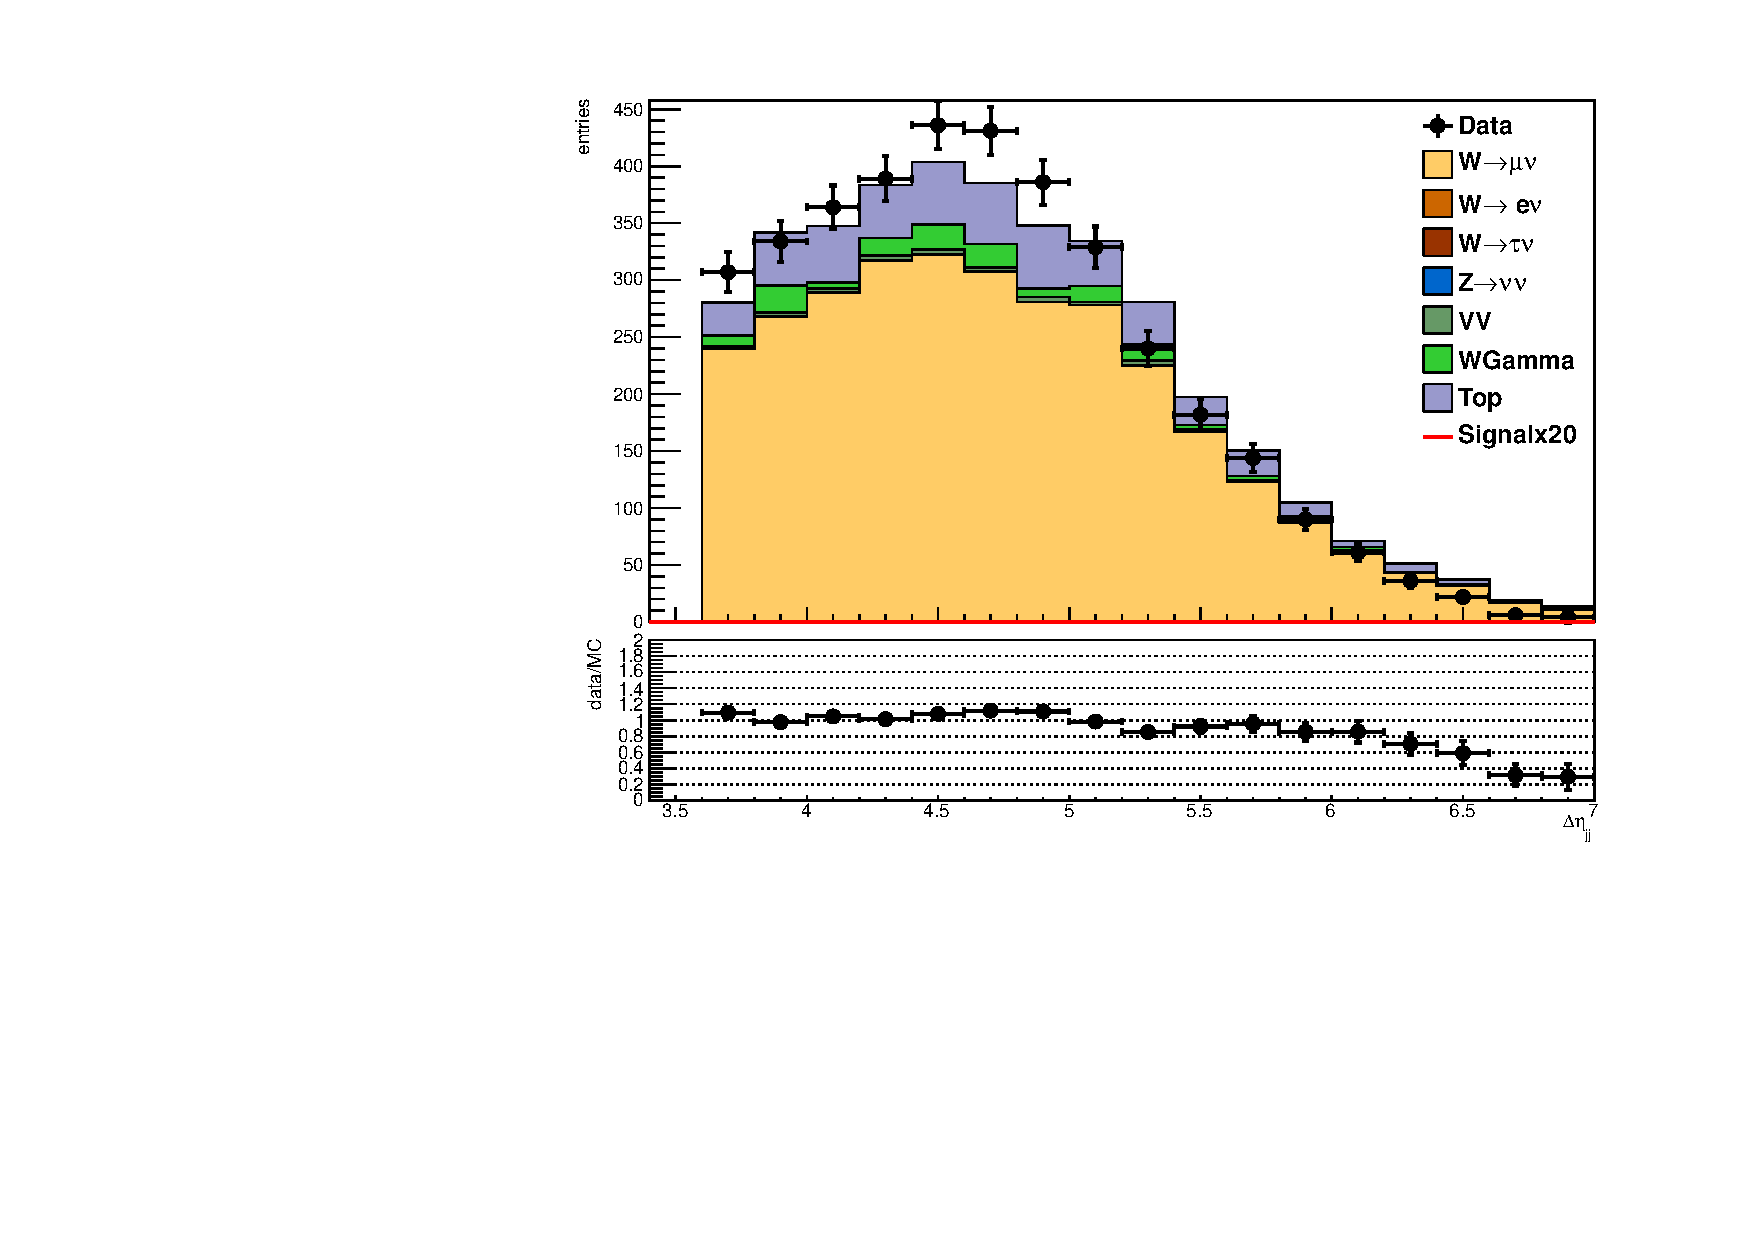
\includegraphics[width=\textwidth]{TalkPics/contplotsandpresel220914/output_contplots_rebinned2dweights/munu_dijet_deta.pdf}
    \end{block}

  \end{columns}
\end{frame}

\begin{frame}
  \frametitle{New control plots - munu}
  \begin{columns}
    \column{.5\textwidth}
    \begin{block}{Leading jets-met mindphi}
      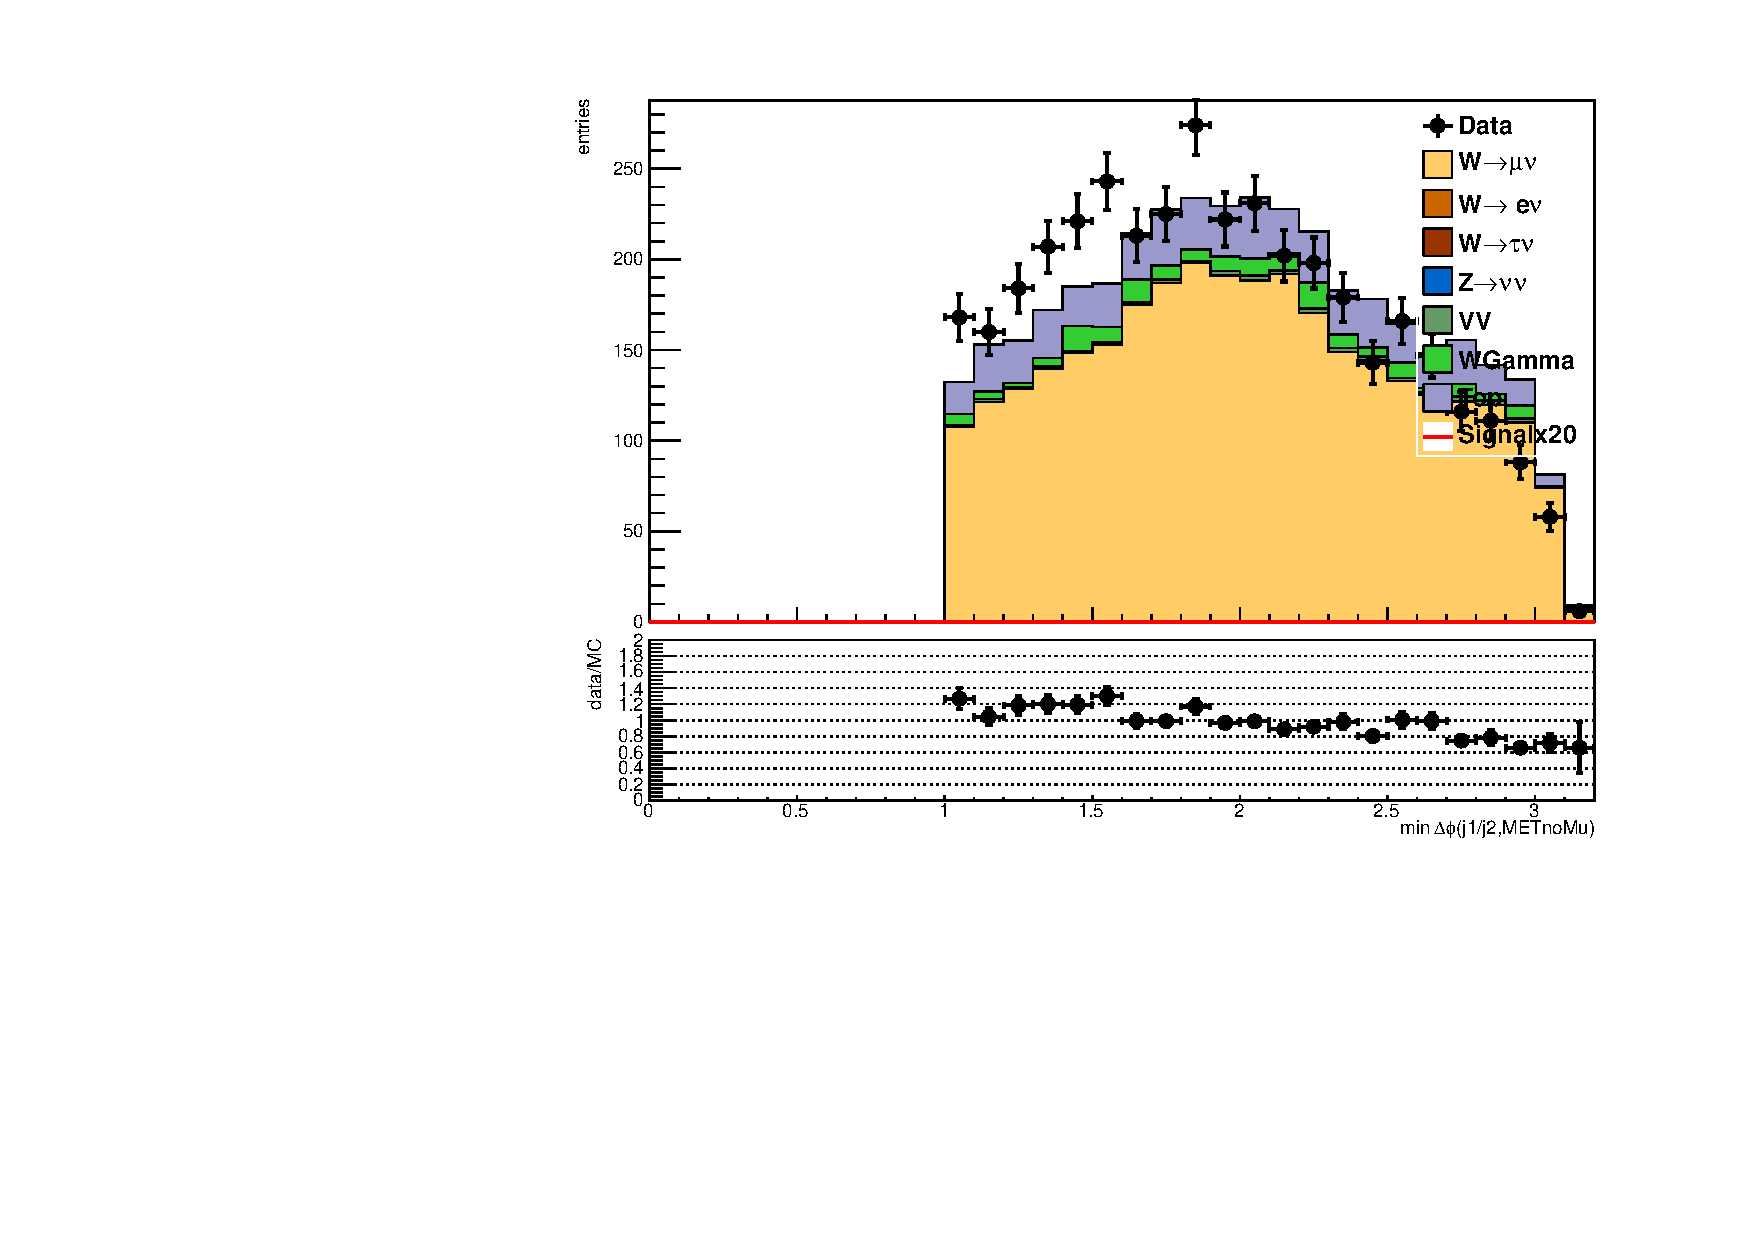
\includegraphics[width=\textwidth]{TalkPics/contplotsandpresel220914/output_contplots_rebinned2dweights/munu_jetmetnomu_mindphi.pdf}
    \end{block}
    \column{.5\textwidth}
    \begin{block}{All jets-met mindphi}
      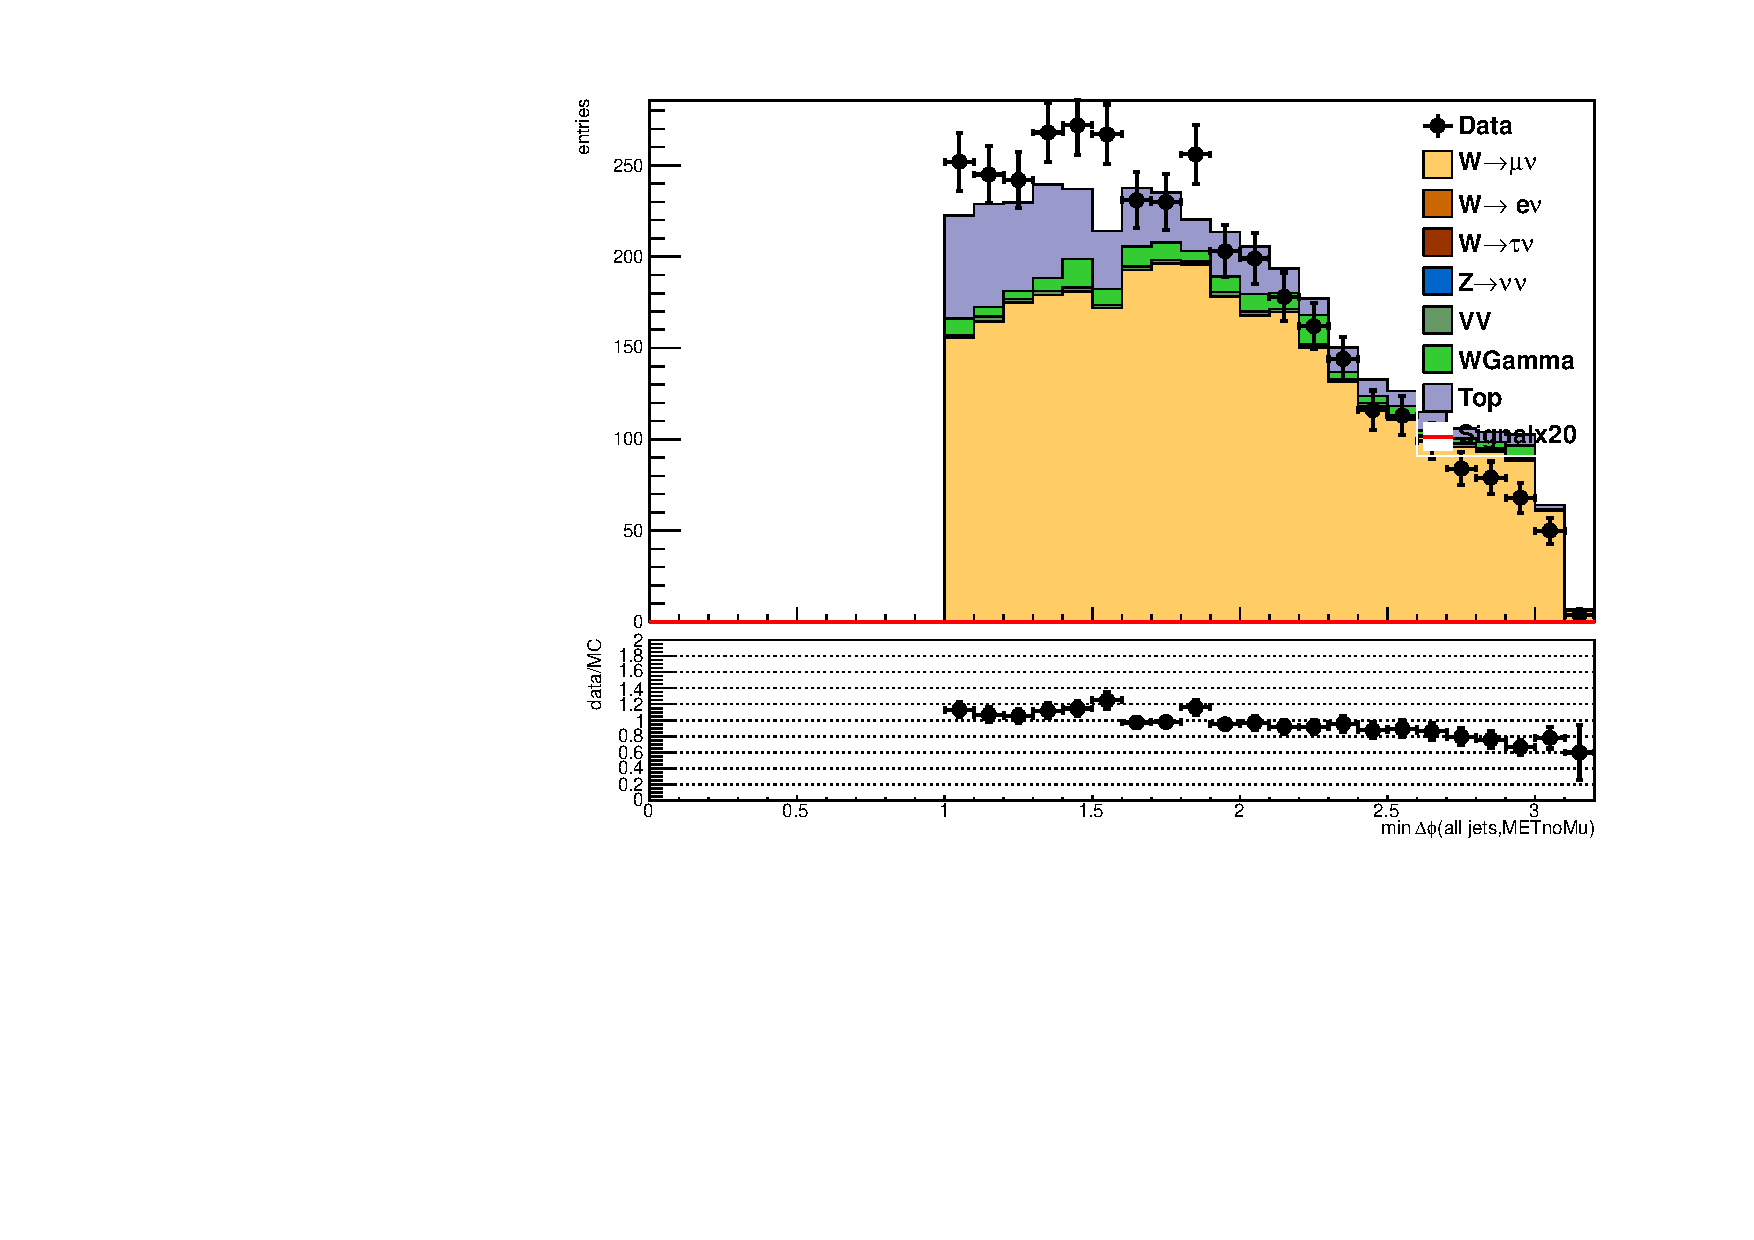
\includegraphics[width=\textwidth]{TalkPics/contplotsandpresel220914/output_contplots_rebinned2dweights/munu_alljetsmetnomu_mindphi.pdf}
    \end{block}

  \end{columns}
\end{frame}

\begin{frame}
  \frametitle{New control plots - munu}
  \begin{columns}
    \column{.5\textwidth}
    \begin{block}{dijet-metnomu pt fraction}
      \includegraphics[width=\textwidth]{TalkPics/contplotsandpresel220914/output_contplots_rebinned2dweights/munu_dijetmetnomu_ptfraction.pdf}
    \end{block}
  \end{columns}
\end{frame}

\begin{frame}
  \frametitle{New control plots - taunu}
  \begin{columns}
    \column{.5\textwidth}
    \begin{block}{Jet 1 pt}
      \includegraphics[width=\textwidth]{TalkPics/contplotsandpresel220914/output_contplots_rebinned2dweights/taunu_jet1_pt.pdf}
    \end{block}
    \column{.5\textwidth}
    \begin{block}{Jet 2 pt}
      \includegraphics[width=\textwidth]{TalkPics/contplotsandpresel220914/output_contplots_rebinned2dweights/taunu_jet2_pt.pdf}
    \end{block}

  \end{columns}
\end{frame}

\begin{frame}
  \frametitle{New control plots - taunu}
  \begin{columns}
    \column{.5\textwidth}
    \begin{block}{METnomu}
      \includegraphics[width=\textwidth]{TalkPics/contplotsandpresel220914/output_contplots_rebinned2dweights/taunu_metnomuons.pdf}
    \end{block}
    \column{.5\textwidth}
    \begin{block}{METnomusig}
      \includegraphics[width=\textwidth]{TalkPics/contplotsandpresel220914/output_contplots_rebinned2dweights/taunu_metnomu_significance.pdf}
    \end{block}

  \end{columns}
\end{frame}

\begin{frame}
  \frametitle{New control plots - taunu}
  \begin{columns}
    \column{.5\textwidth}
    \begin{block}{Mjj}
      \includegraphics[width=\textwidth]{TalkPics/contplotsandpresel220914/output_contplots_rebinned2dweights/taunu_dijet_M.pdf}
    \end{block}
    \column{.5\textwidth}
    \begin{block}{mt}
      \includegraphics[width=\textwidth]{TalkPics/contplotsandpresel220914/output_contplots_rebinned2dweights/taunu_lep_mt.pdf}
    \end{block}
  \end{columns}
\end{frame}

\begin{frame}
  \frametitle{New control plots - taunu}
  \begin{columns}
    \column{.5\textwidth}
    \begin{block}{Dijet Dphi}
      \includegraphics[width=\textwidth]{TalkPics/contplotsandpresel220914/output_contplots_rebinned2dweights/taunu_dijet_dphi.pdf}
    \end{block}
    \column{.5\textwidth}
    \begin{block}{Detajj}
      \includegraphics[width=\textwidth]{TalkPics/contplotsandpresel220914/output_contplots_rebinned2dweights/taunu_dijet_deta.pdf}
    \end{block}

  \end{columns}
\end{frame}

\begin{frame}
  \frametitle{New control plots - taunu}
  \begin{columns}
    \column{.5\textwidth}
    \begin{block}{Leading jets-met mindphi}
      \includegraphics[width=\textwidth]{TalkPics/contplotsandpresel220914/output_contplots_rebinned2dweights/taunu_jetmetnomu_mindphi.pdf}
    \end{block}
    \column{.5\textwidth}
    \begin{block}{All jets-met mindphi}
      \includegraphics[width=\textwidth]{TalkPics/contplotsandpresel220914/output_contplots_rebinned2dweights/taunu_alljetsmetnomu_mindphi.pdf}
    \end{block}

  \end{columns}
\end{frame}

\begin{frame}
  \frametitle{New control plots - taunu}
  \begin{columns}
    \column{.5\textwidth}
    \begin{block}{dijet-metnomu pt fraction}
      \includegraphics[width=\textwidth]{TalkPics/contplotsandpresel220914/output_contplots_rebinned2dweights/taunu_dijetmetnomu_ptfraction.pdf}
    \end{block}
  \end{columns}
\end{frame}

\end{fmffile}
\end{document}
